%%____________________________________________________________________________||
\section{Interpretation in Simplified SUSY models}
\label{app:susy}

\subsection{Signal distribution}
\label{app:susy-mr-plots}

%\subsubsection{Nominal analysis binning}
%
%\begin{figure}[!h]
%    \centering
%    \subfigure[Monojet]{
%        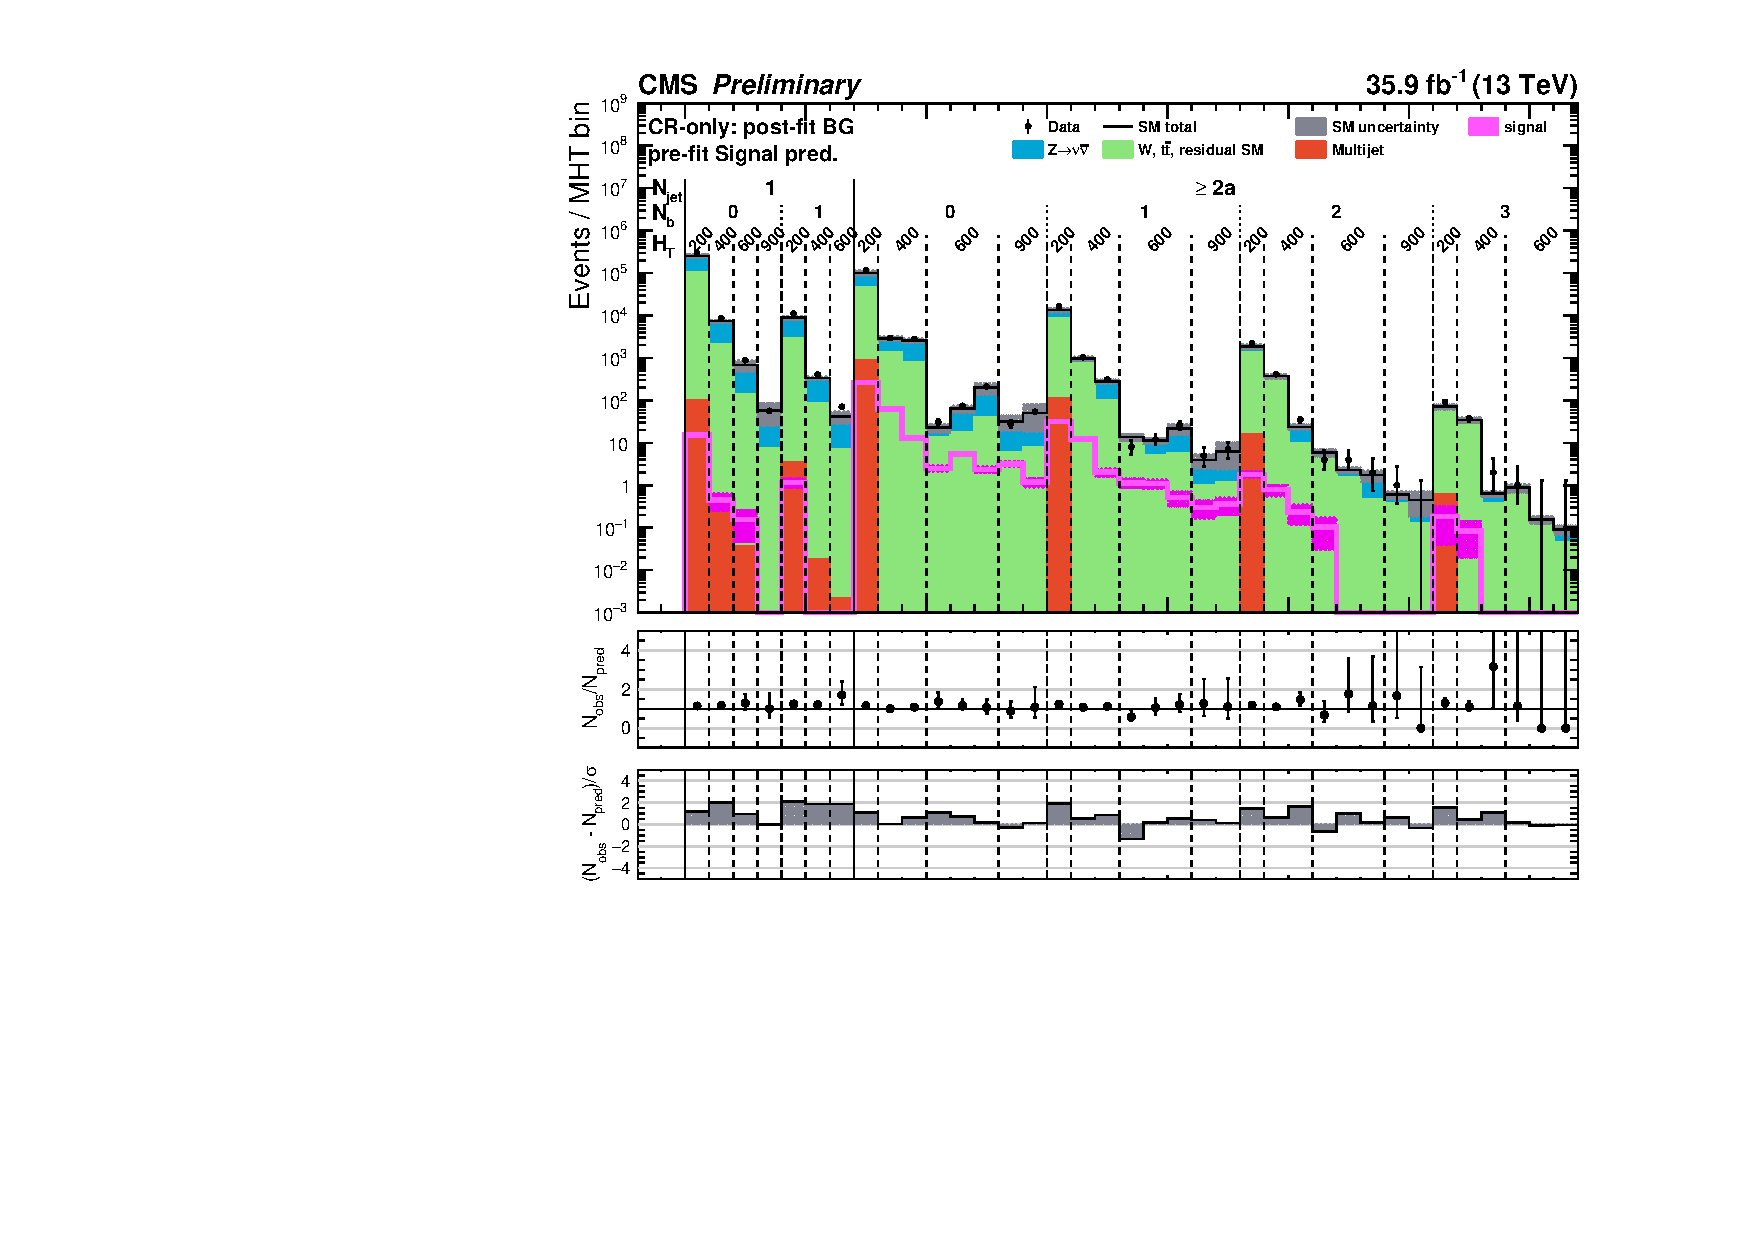
\includegraphics[width=0.49\textwidth]{figures/susyResults/app/T1qqqq_mGluino-1000_mLSP-850/monojet_full-fit-sig}
%        \label{fig:T1qqqq_compressed_MR_1j}
%    } ~~
%    \subfigure[Di-jet]{
%        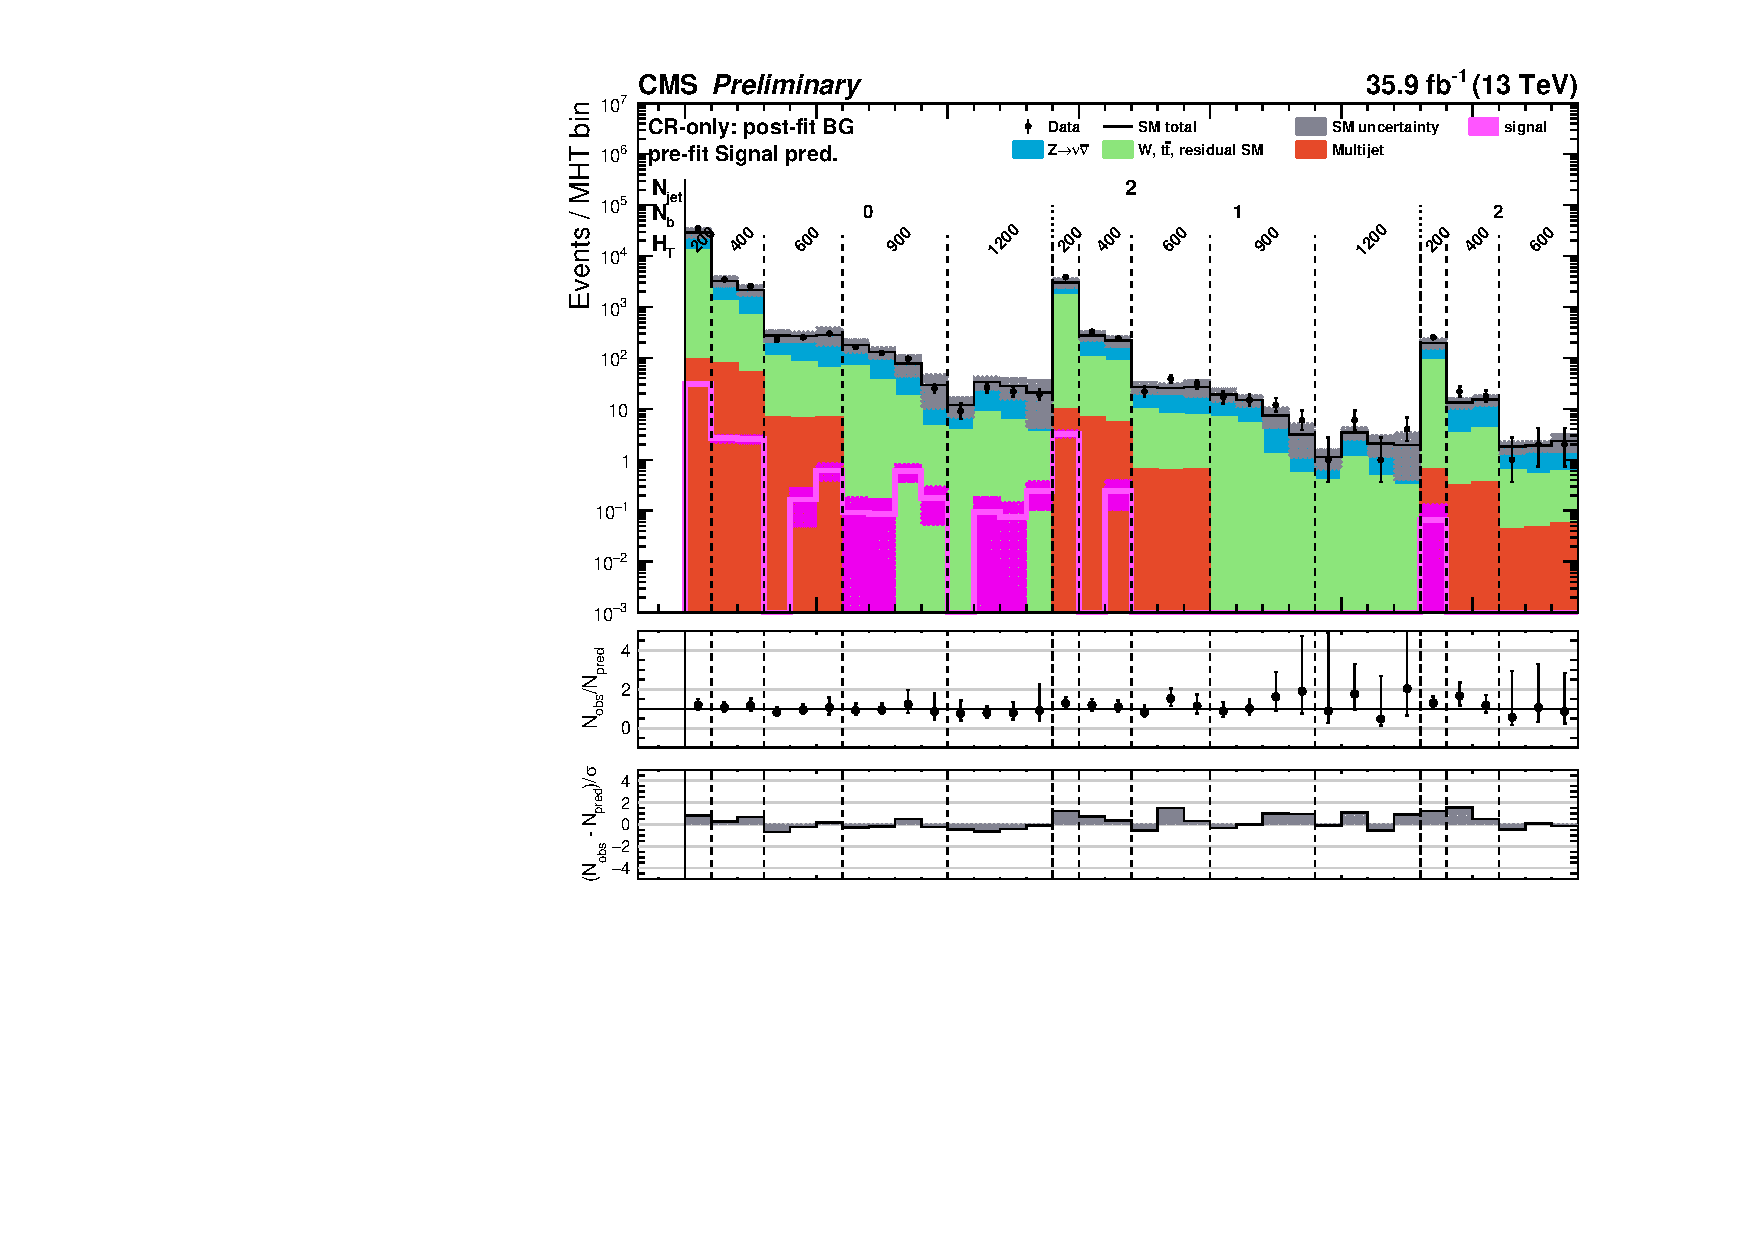
\includegraphics[width=0.49\textwidth]{figures/susyResults/app/T1qqqq_mGluino-1000_mLSP-850/di-jet_full-fit-sig}
%        \label{fig:T1qqqq_compressed_MR_2j}
%    } \\
%    \subfigure[3 jet]{
%        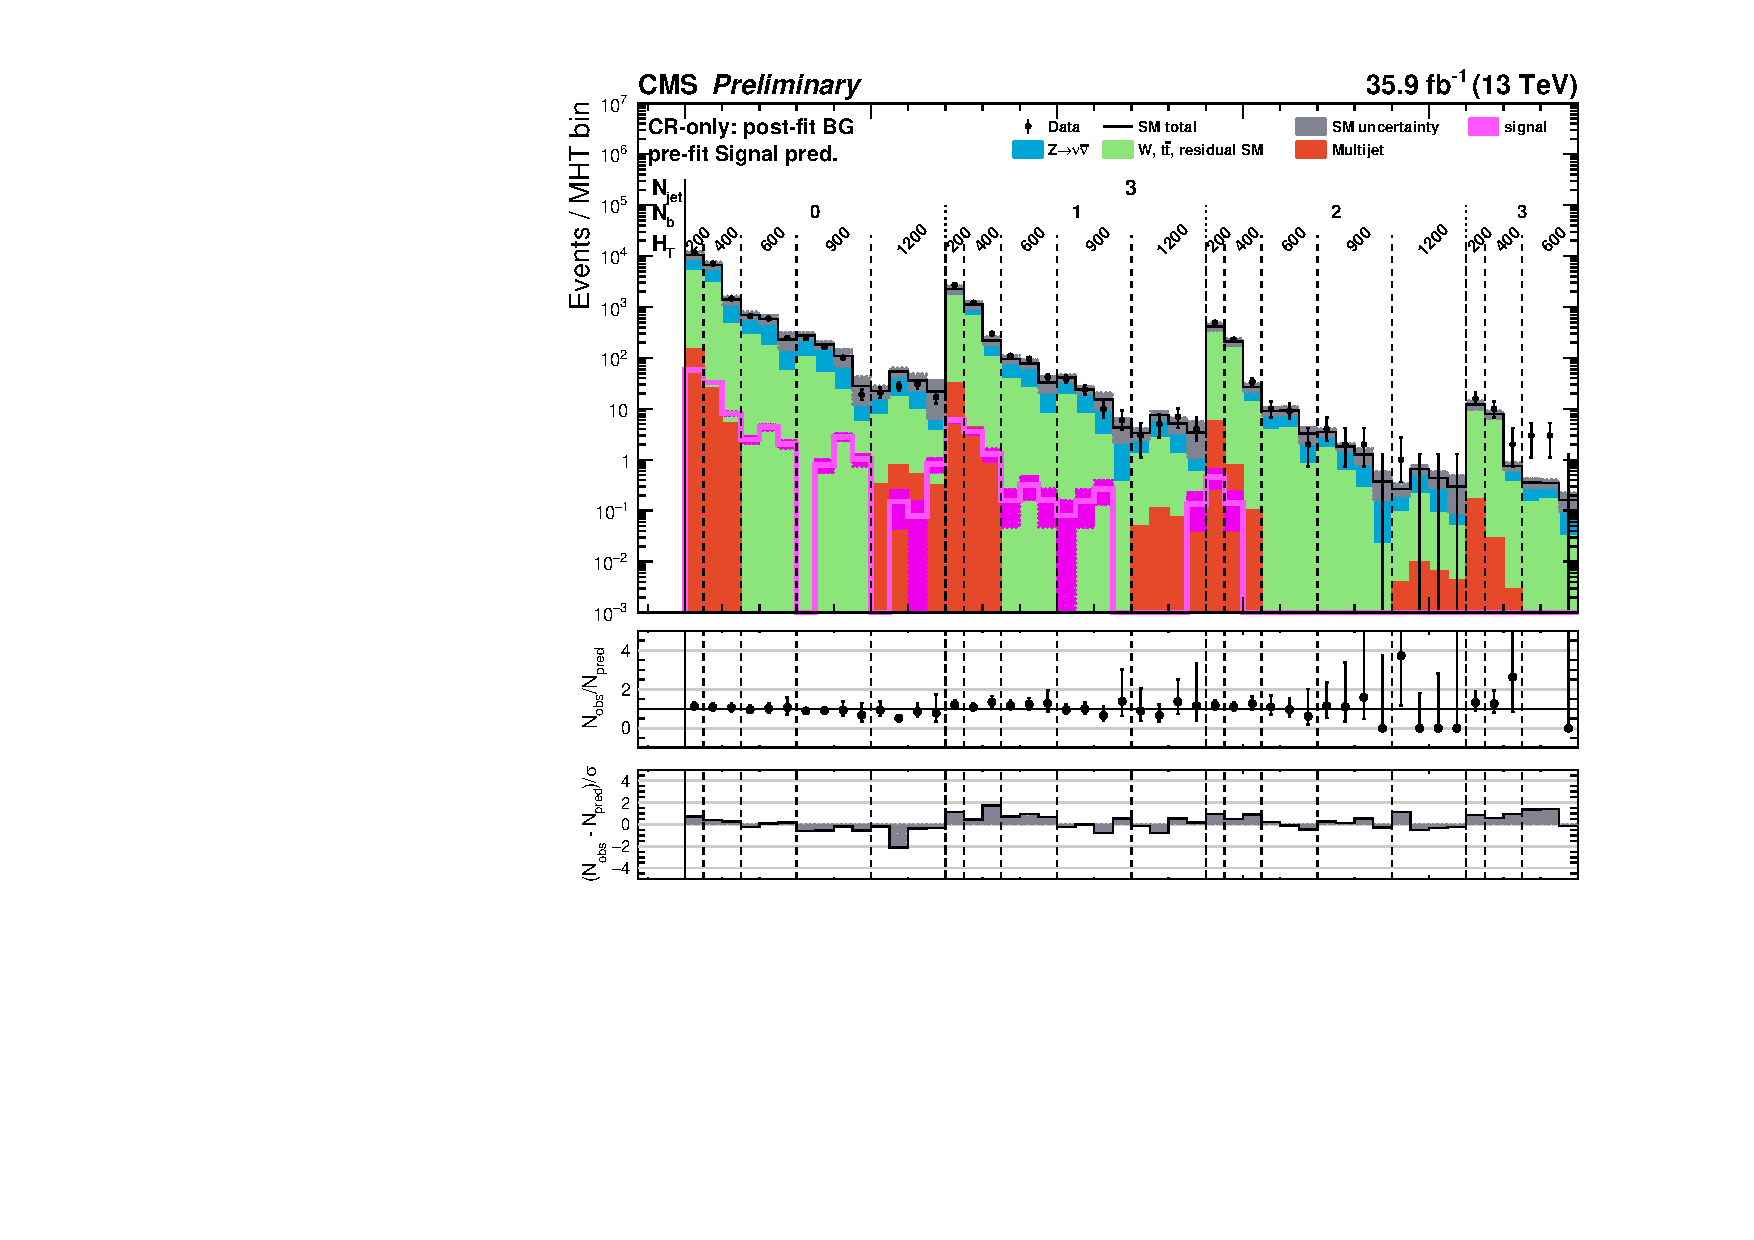
\includegraphics[width=0.49\textwidth]{figures/susyResults/app/T1qqqq_mGluino-1000_mLSP-850/3jet_full-fit-sig}
%        \label{fig:T1qqqq_compressed_MR_3j}
%    } ~~
%    \subfigure[4 jet]{
%        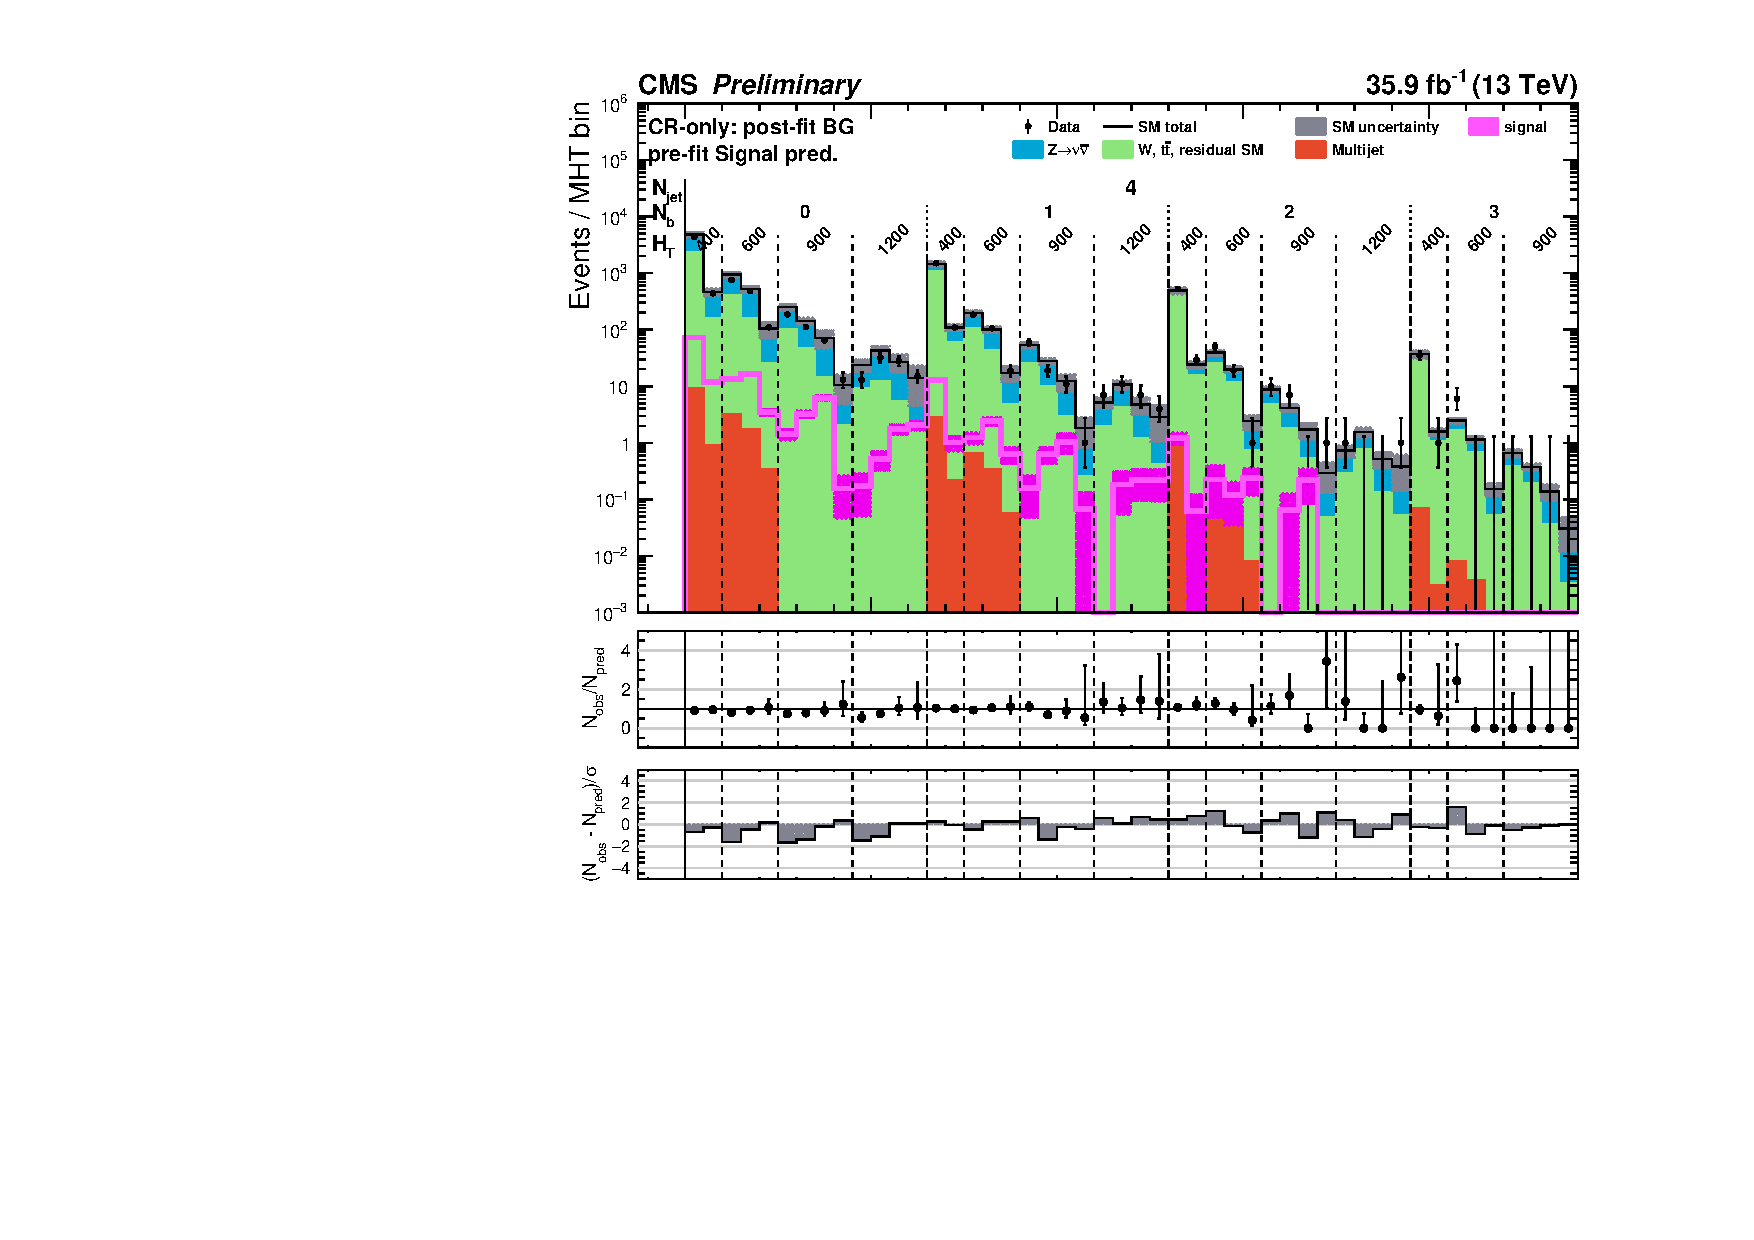
\includegraphics[width=0.49\textwidth]{figures/susyResults/app/T1qqqq_mGluino-1000_mLSP-850/4jet_full-fit-sig}
%        \label{fig:T1qqqq_compressed_MR_4j}
%    } \\
%    \subfigure[5 jet]{
%        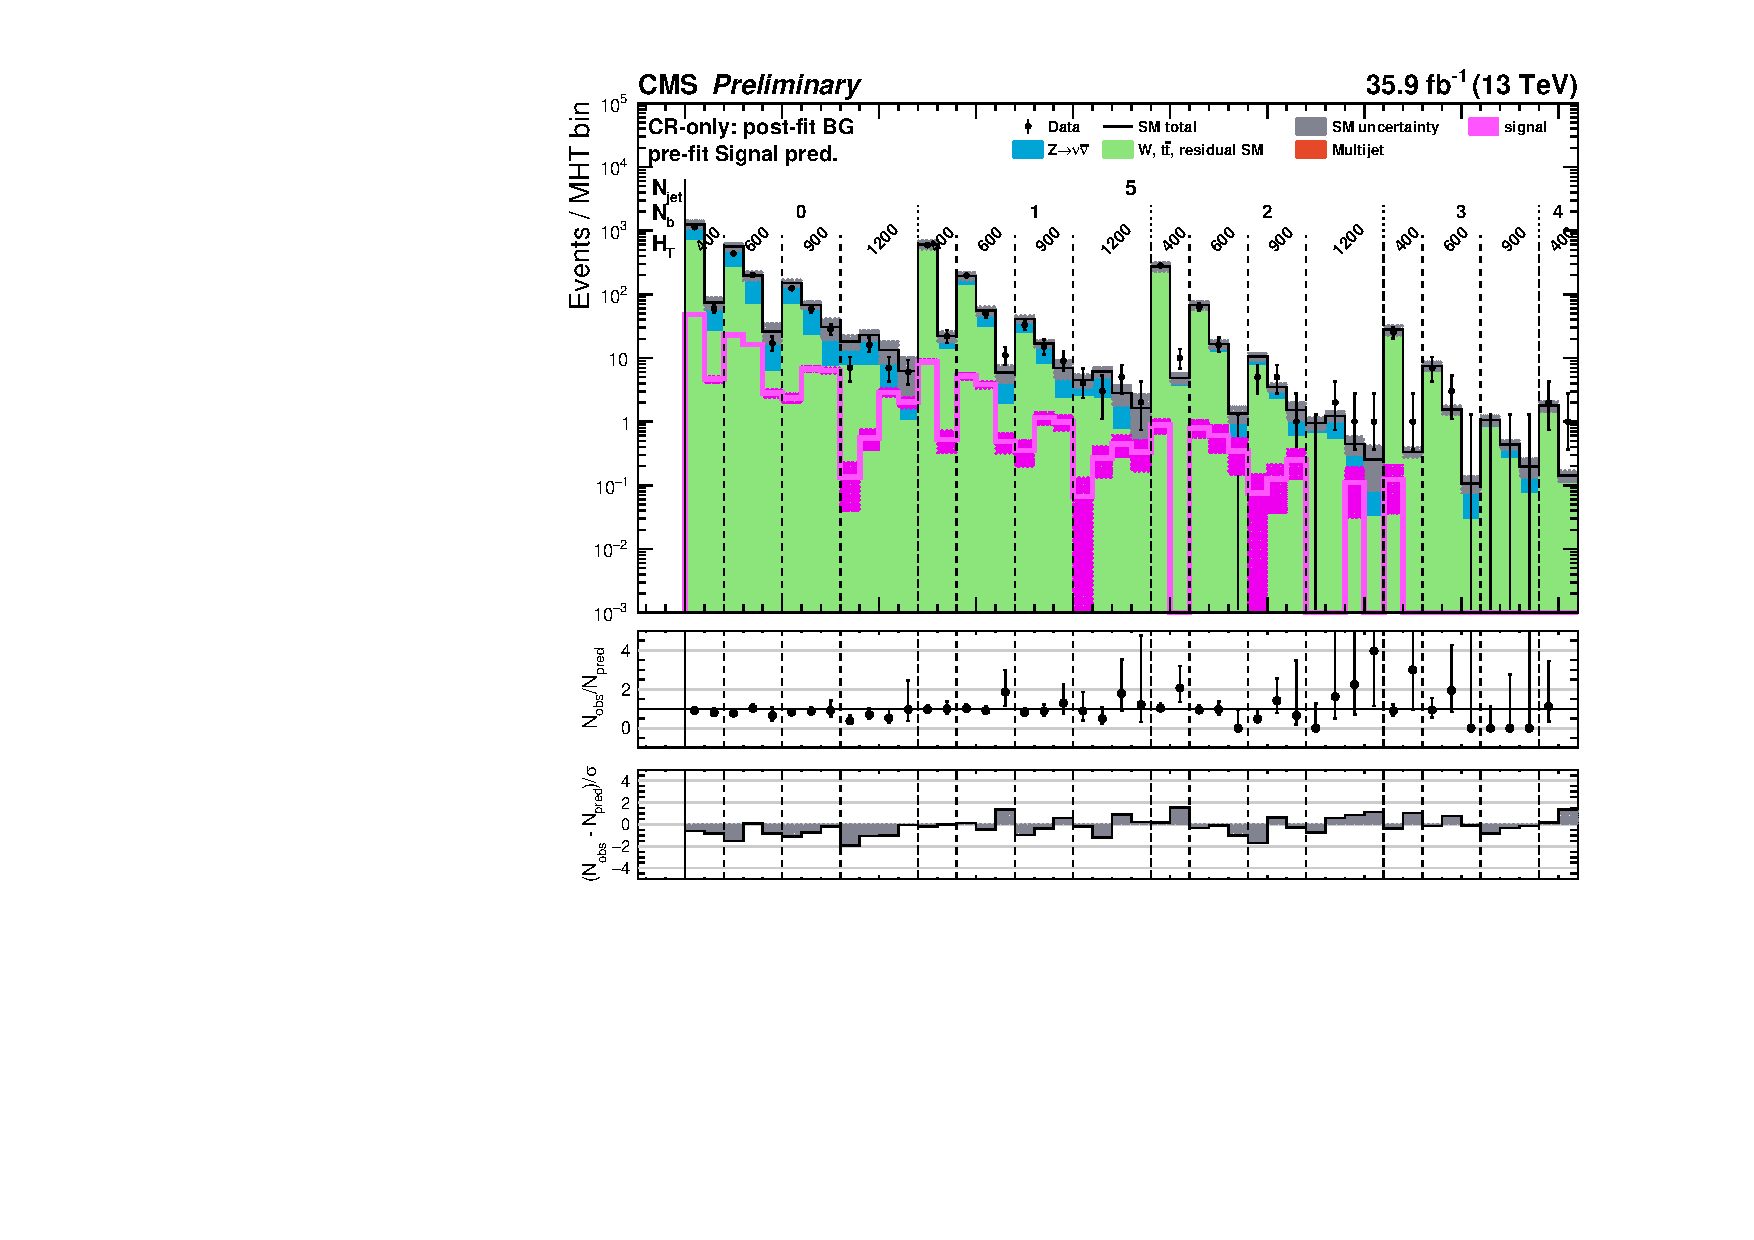
\includegraphics[width=0.49\textwidth]{figures/susyResults/app/T1qqqq_mGluino-1000_mLSP-850/5jet_full-fit-sig}
%        \label{fig:T1qqqq_compressed_MR_5j}
%    } ~~
%    \subfigure[6+ jet]{
%        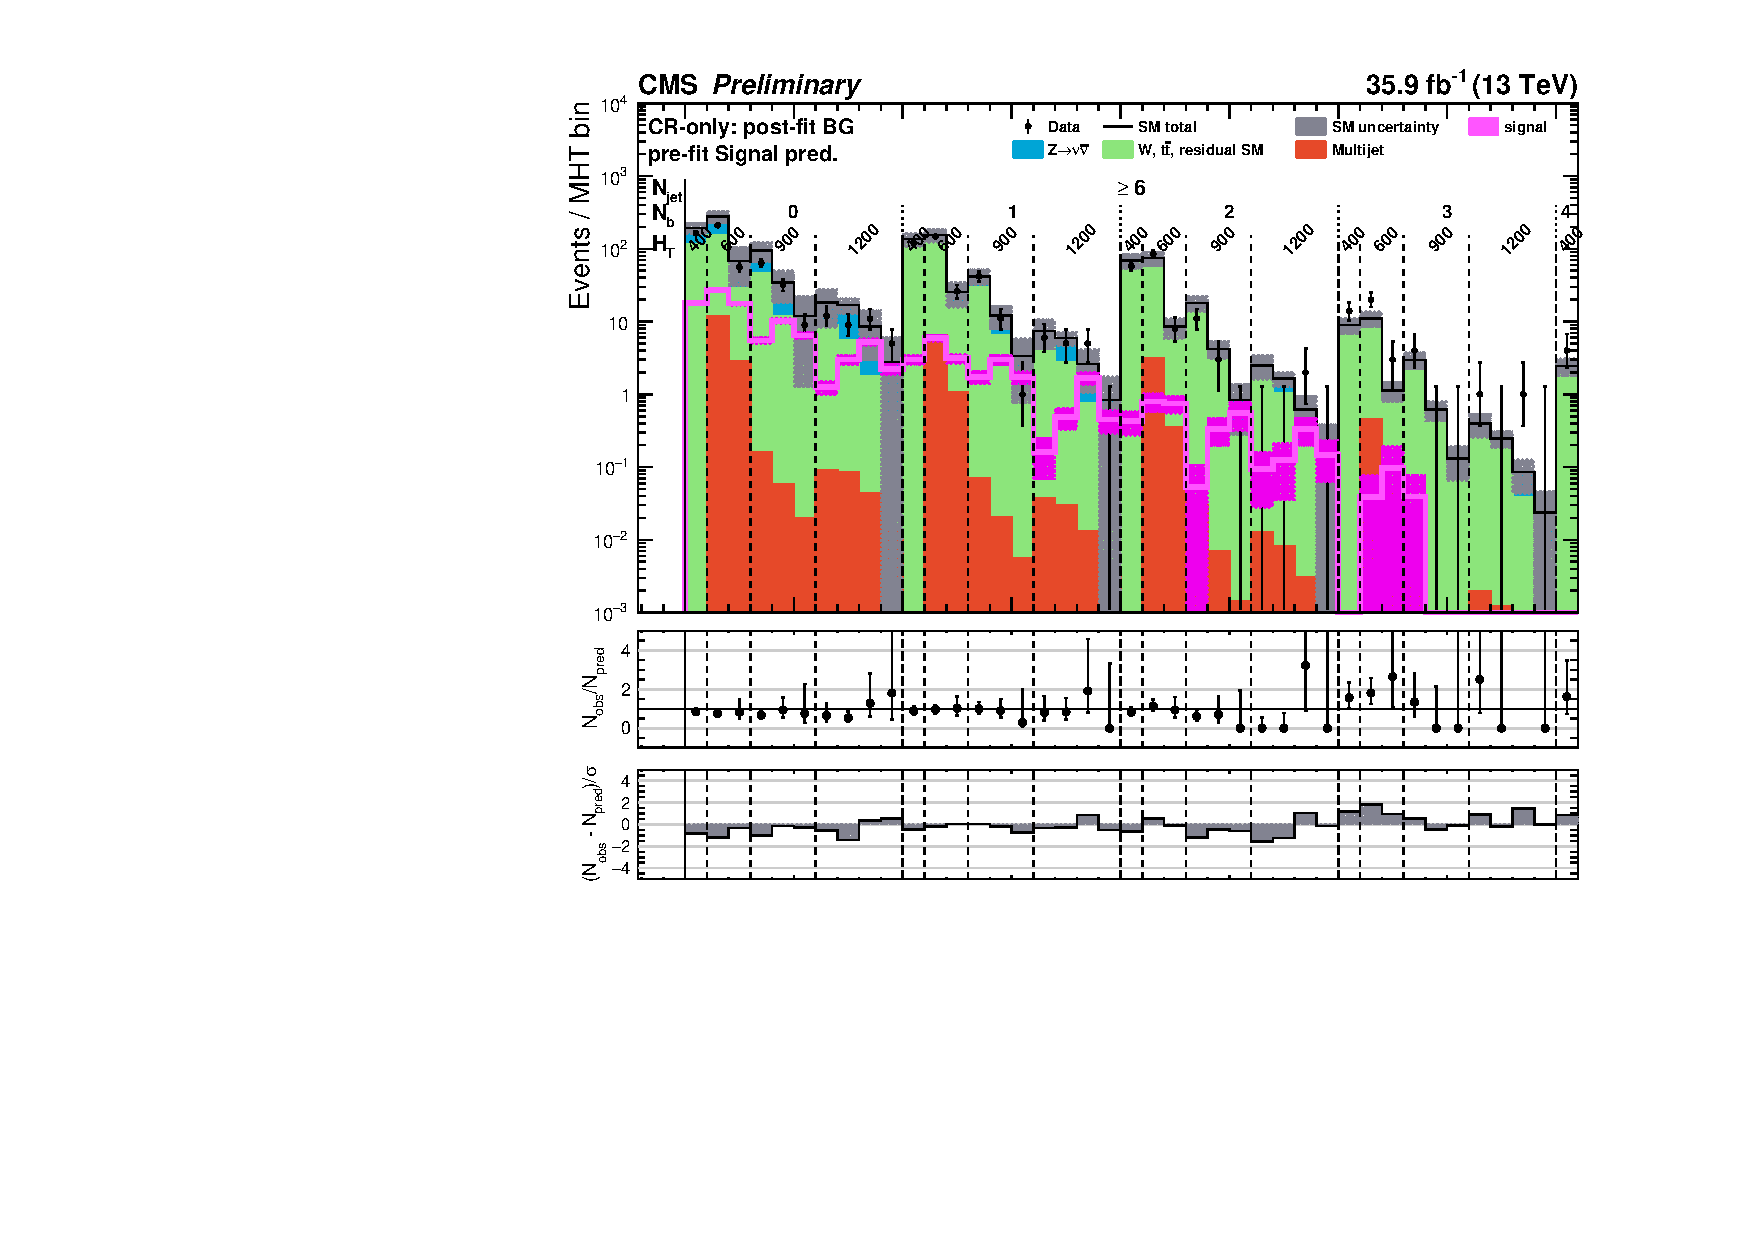
\includegraphics[width=0.49\textwidth]{figures/susyResults/app/T1qqqq_mGluino-1000_mLSP-850/6+_jets_full-fit-sig}
%        \label{fig:T1qqqq_compressed_MR_6j}
%    } \\
%    \caption{
%        Pre-fit T1qqqq compressed $(1000,850)$ benchmark model overlay on
%        CR-only post-fit background prediction for all analysis bins. The
%        uncertainty on the signal model counts represents the statistical
%        uncertainty due to the finite size of the of the simulated sample.
%    }
%    \label{fig:T1qqqq_compressed_MR}
%\end{figure}
%
%\begin{figure}[!h]
%    \centering
%    \subfigure[Monojet]{
%        \includegraphics[width=0.49\textwidth]{figures/susyResults/app/T1qqqq_mGluino-1700_mLSP-100/monojet_full-fit-sig}
%        \label{fig:T1qqqq_uncompressed_MR_1j}
%    } ~~
%    \subfigure[Di-jet]{
%        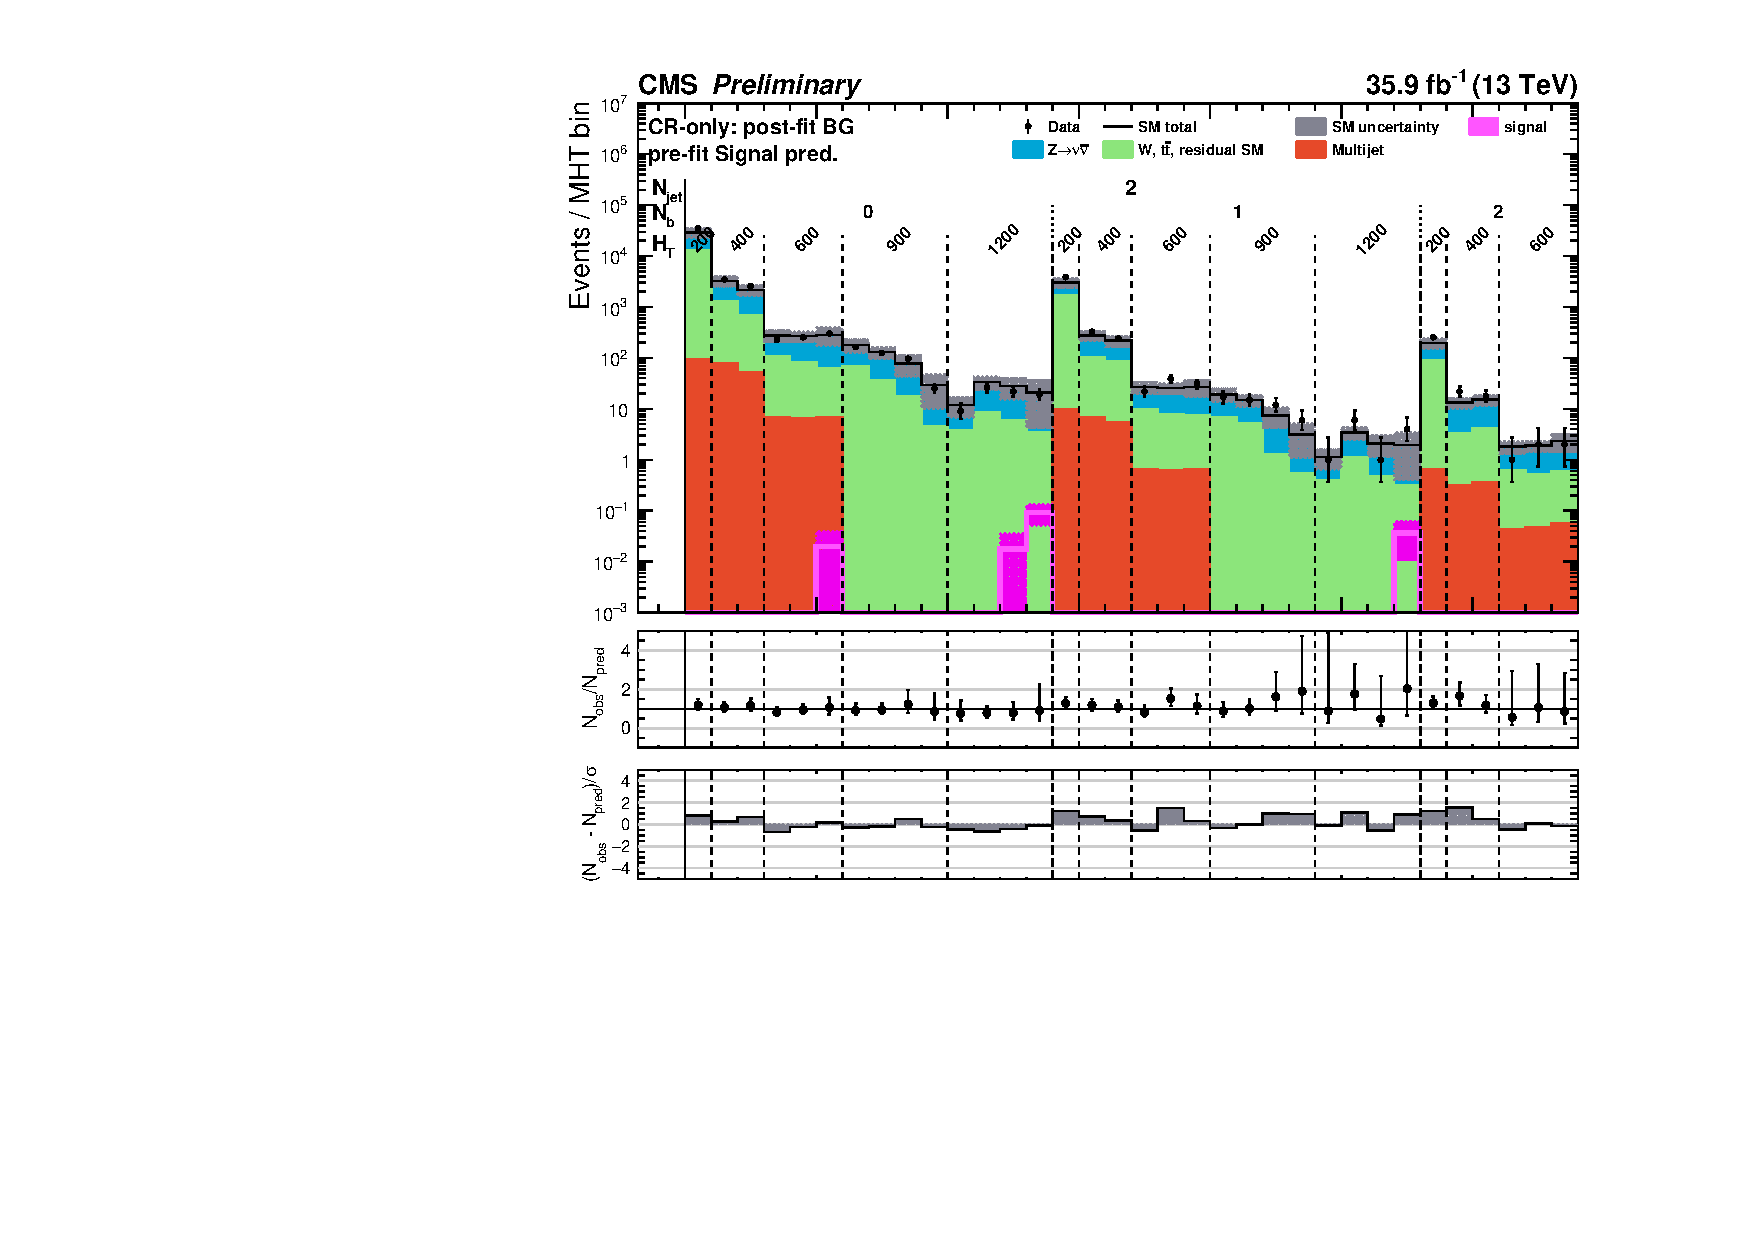
\includegraphics[width=0.49\textwidth]{figures/susyResults/app/T1qqqq_mGluino-1700_mLSP-100/di-jet_full-fit-sig}
%        \label{fig:T1qqqq_uncompressed_MR_2j}
%    } \\
%    \subfigure[3 jet]{
%        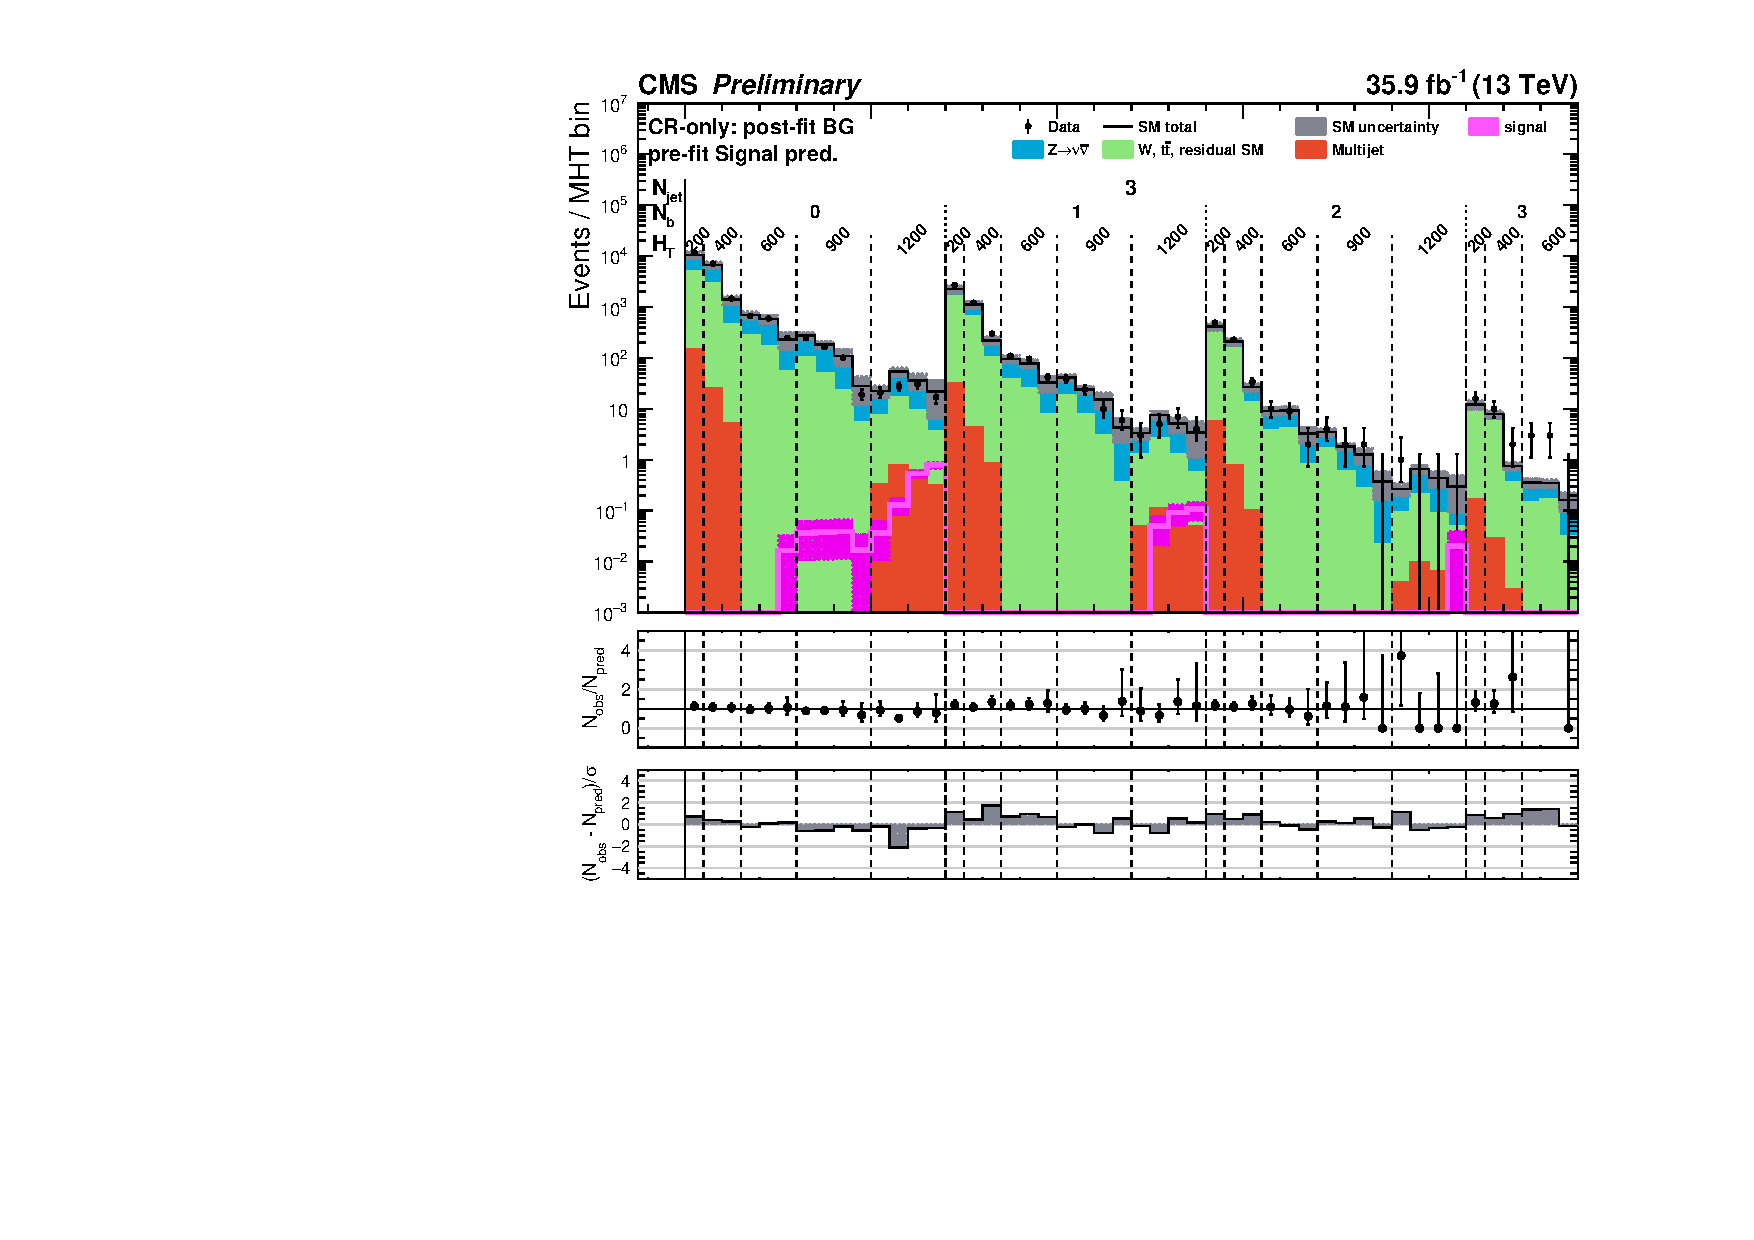
\includegraphics[width=0.49\textwidth]{figures/susyResults/app/T1qqqq_mGluino-1700_mLSP-100/3jet_full-fit-sig}
%        \label{fig:T1qqqq_uncompressed_MR_3j}
%    } ~~
%    \subfigure[4 jet]{
%        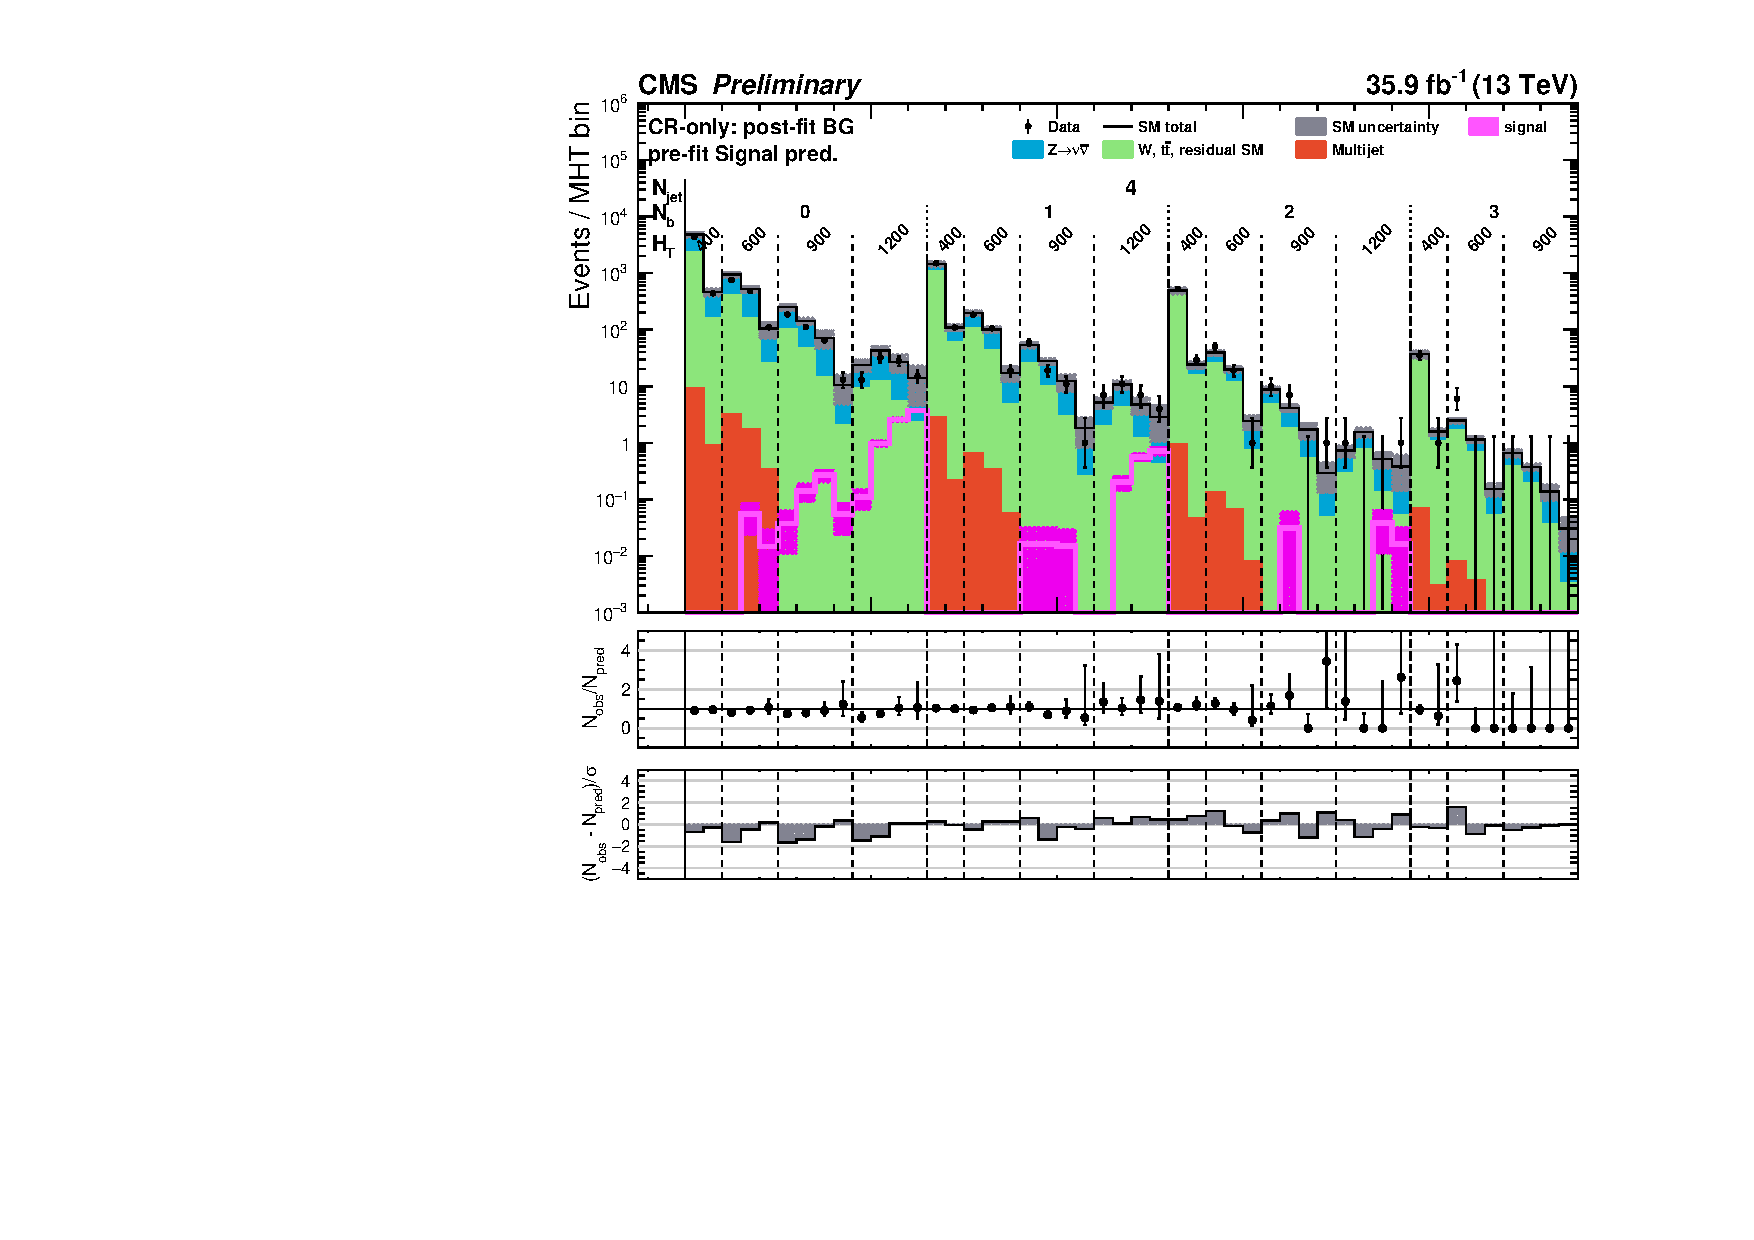
\includegraphics[width=0.49\textwidth]{figures/susyResults/app/T1qqqq_mGluino-1700_mLSP-100/4jet_full-fit-sig}
%        \label{fig:T1qqqq_uncompressed_MR_4j}
%    } \\
%    \subfigure[5 jet]{
%        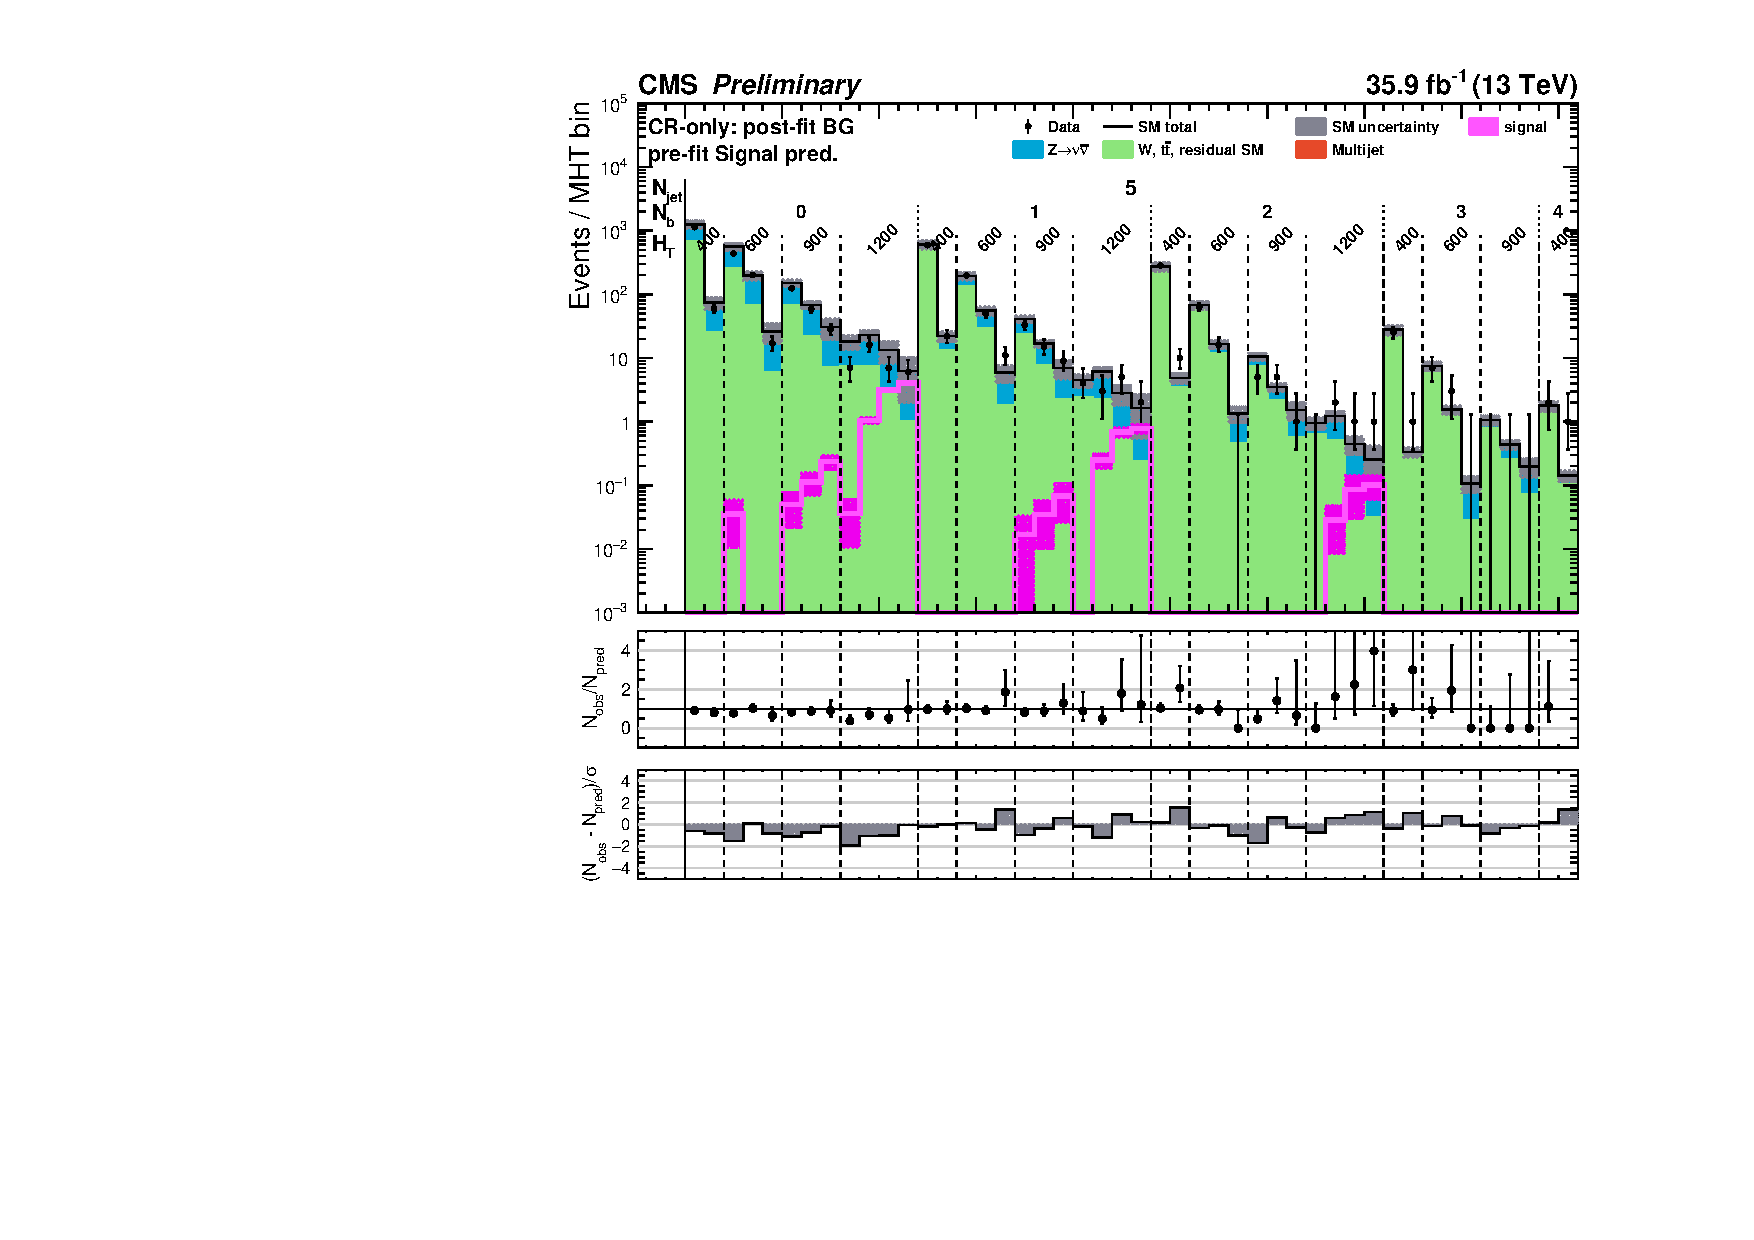
\includegraphics[width=0.49\textwidth]{figures/susyResults/app/T1qqqq_mGluino-1700_mLSP-100/5jet_full-fit-sig}
%        \label{fig:T1qqqq_uncompressed_MR_5j}
%    } ~~
%    \subfigure[6+ jet]{
%        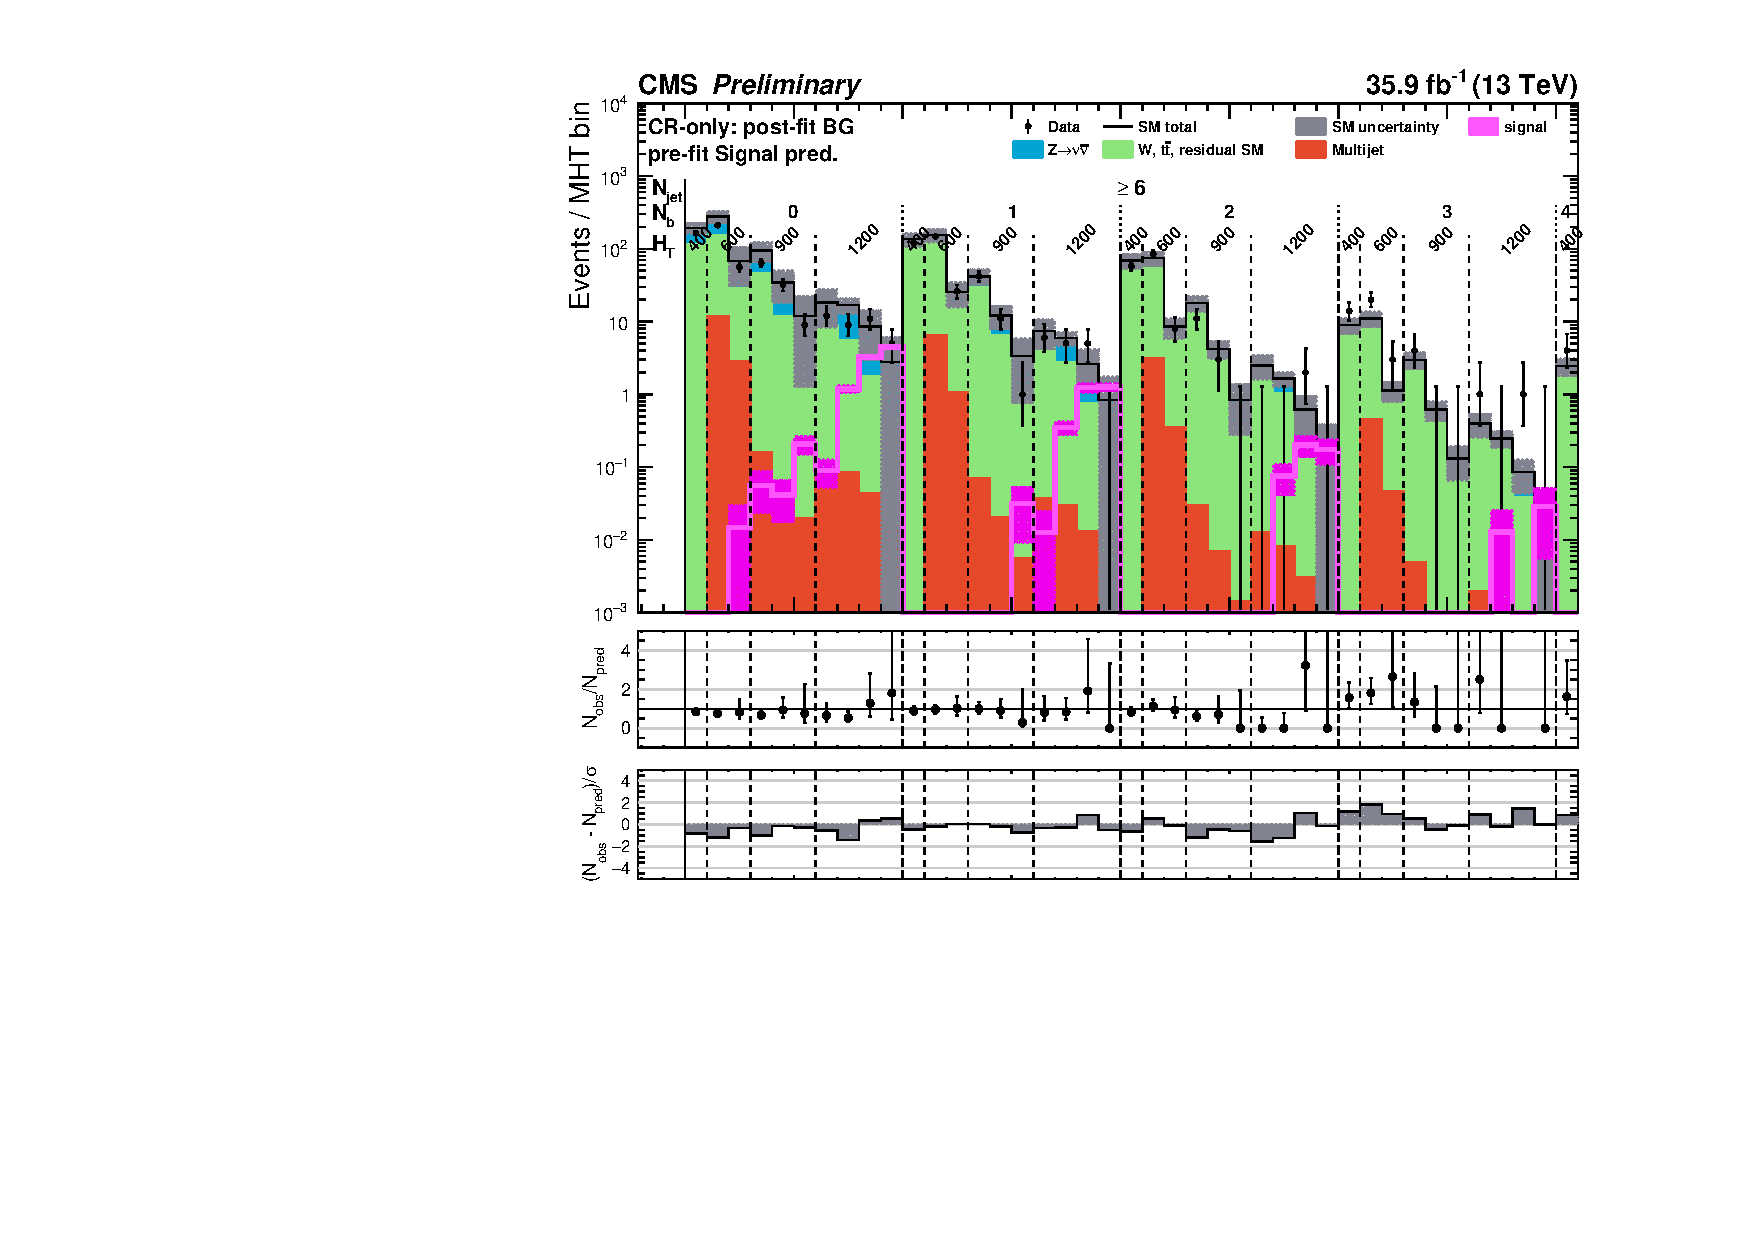
\includegraphics[width=0.49\textwidth]{figures/susyResults/app/T1qqqq_mGluino-1700_mLSP-100/6+_jets_full-fit-sig}
%        \label{fig:T1qqqq_uncompressed_MR_6j}
%    } \\
%    \caption{
%        Pre-fit T1qqqq uncompressed $(1700,100)$ benchmark model overlay on
%        CR-only post-fit background prediction for all analysis bins. The
%        uncertainty on the signal model counts represents the statistical
%        uncertainty due to the finite size of the of the simulated sample.
%    }
%    \label{fig:T1qqqq_uncompressed_MR}
%\end{figure}
%
%\begin{figure}[!h]
%    \centering
%    \subfigure[Monojet]{
%        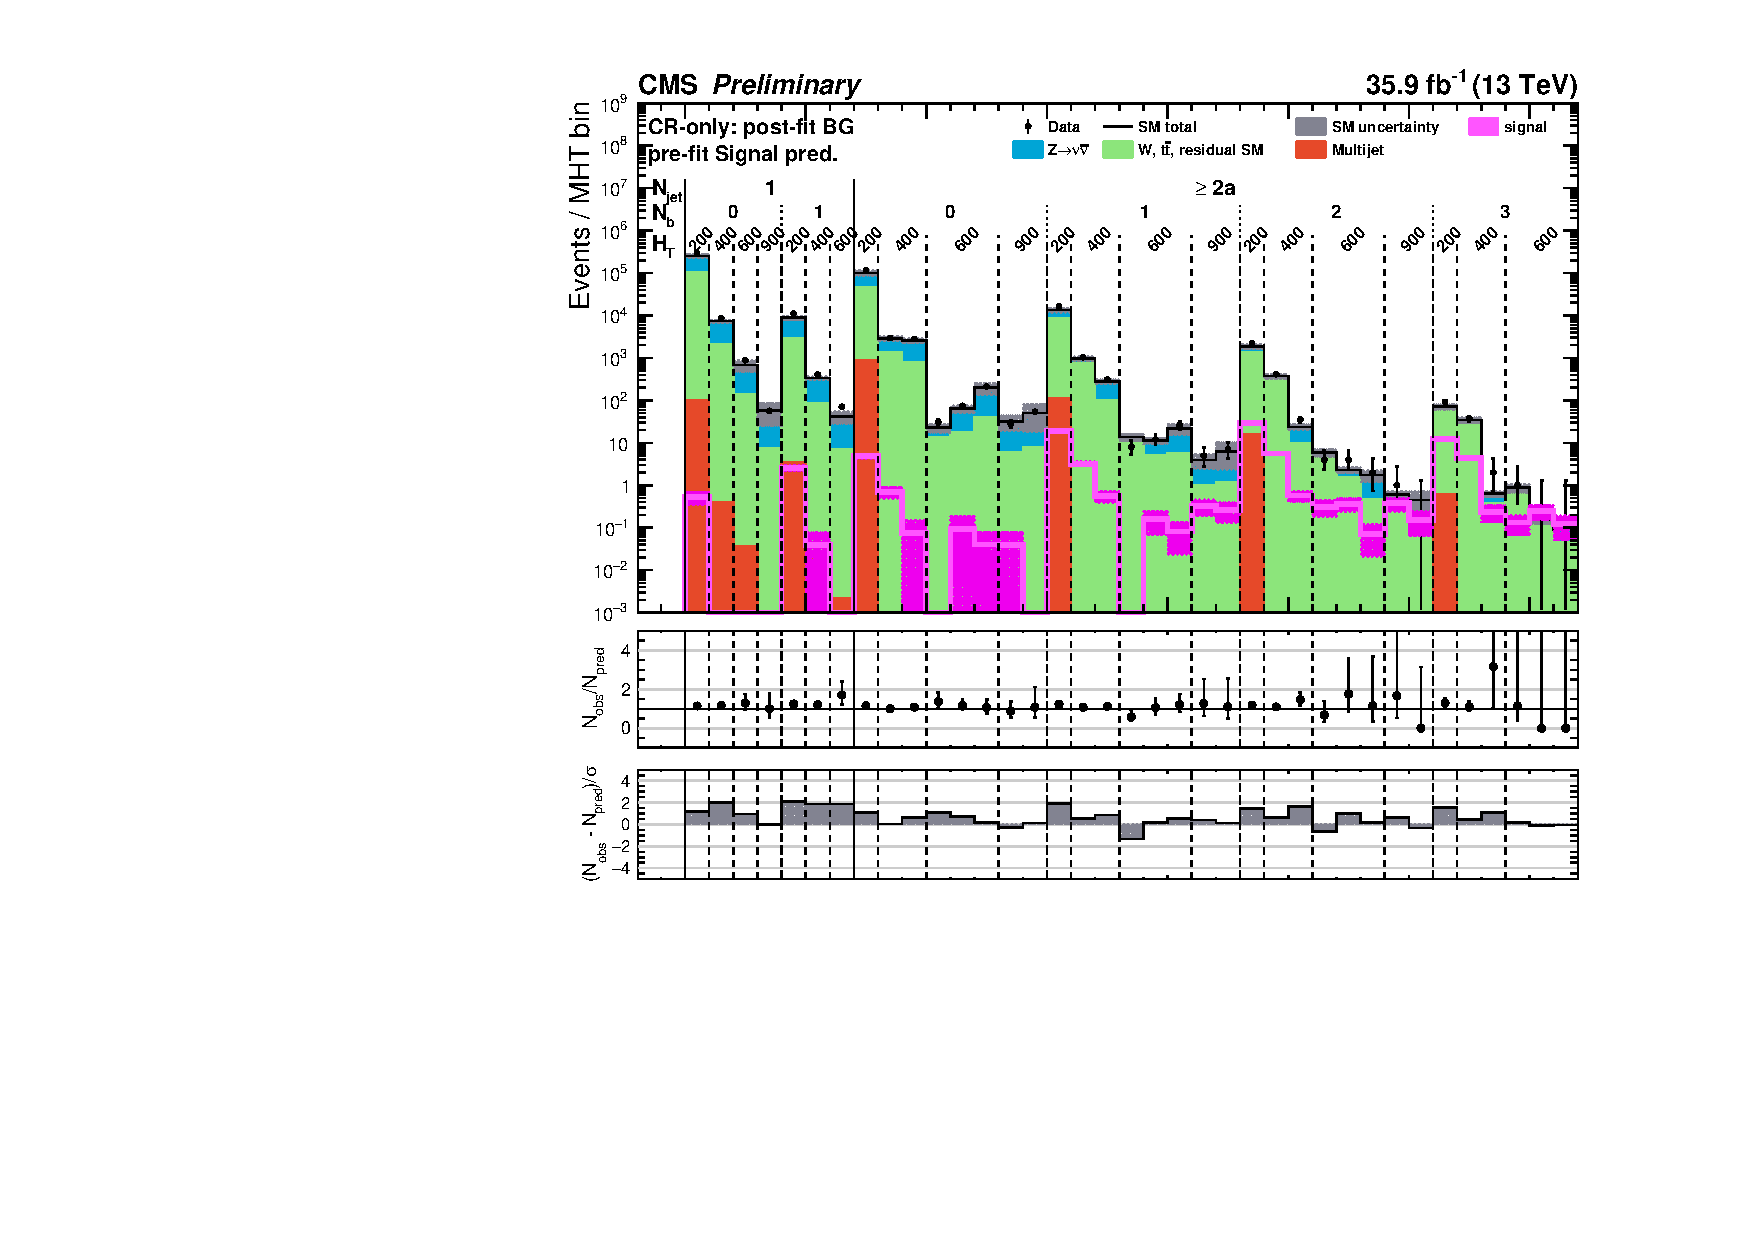
\includegraphics[width=0.49\textwidth]{figures/susyResults/app/T1bbbb_mGluino-1300_mLSP-1100/monojet_full-fit-sig}
%        \label{fig:T1bbbb_compressed_MR_1j}
%    } ~~
%    \subfigure[Di-jet]{
%        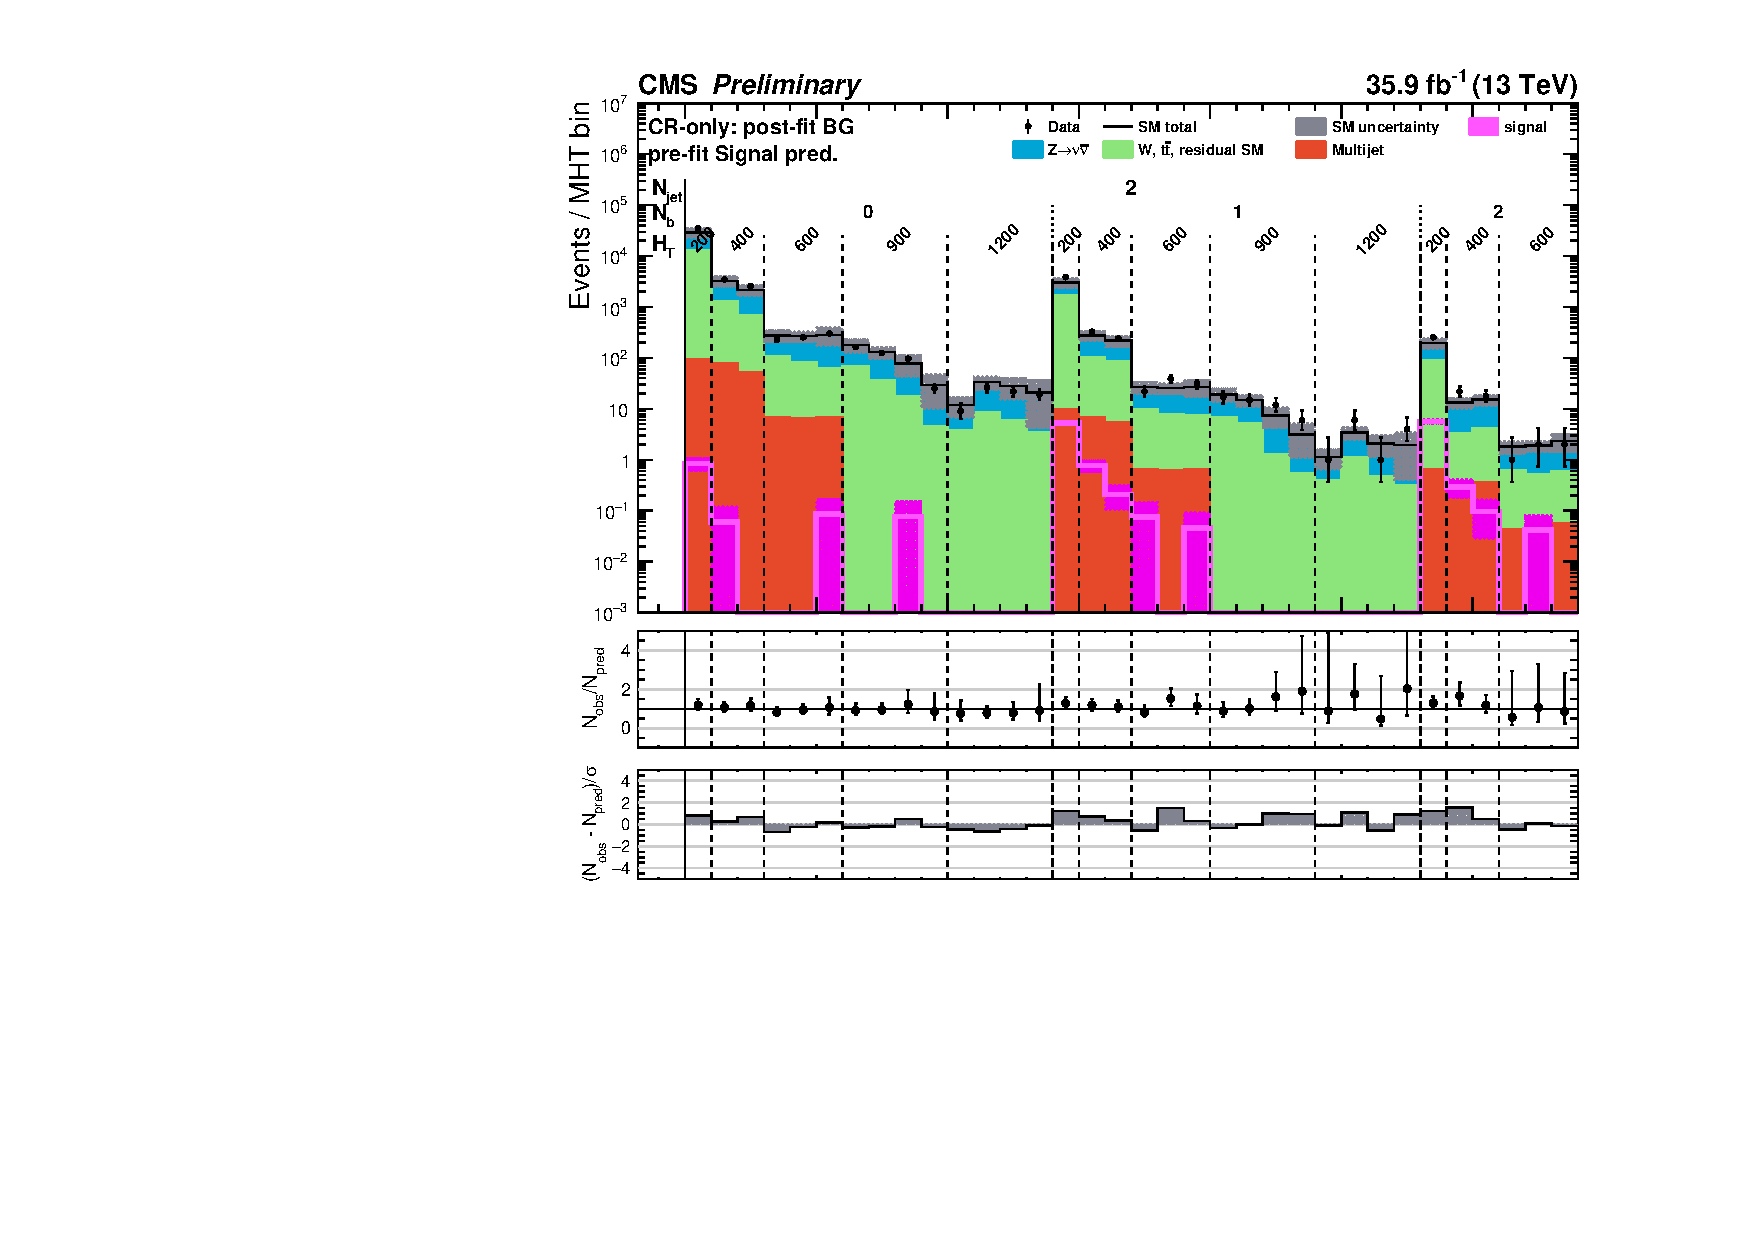
\includegraphics[width=0.49\textwidth]{figures/susyResults/app/T1bbbb_mGluino-1300_mLSP-1100/di-jet_full-fit-sig}
%        \label{fig:T1bbbb_compressed_MR_2j}
%    } \\
%    \subfigure[3 jet]{
%        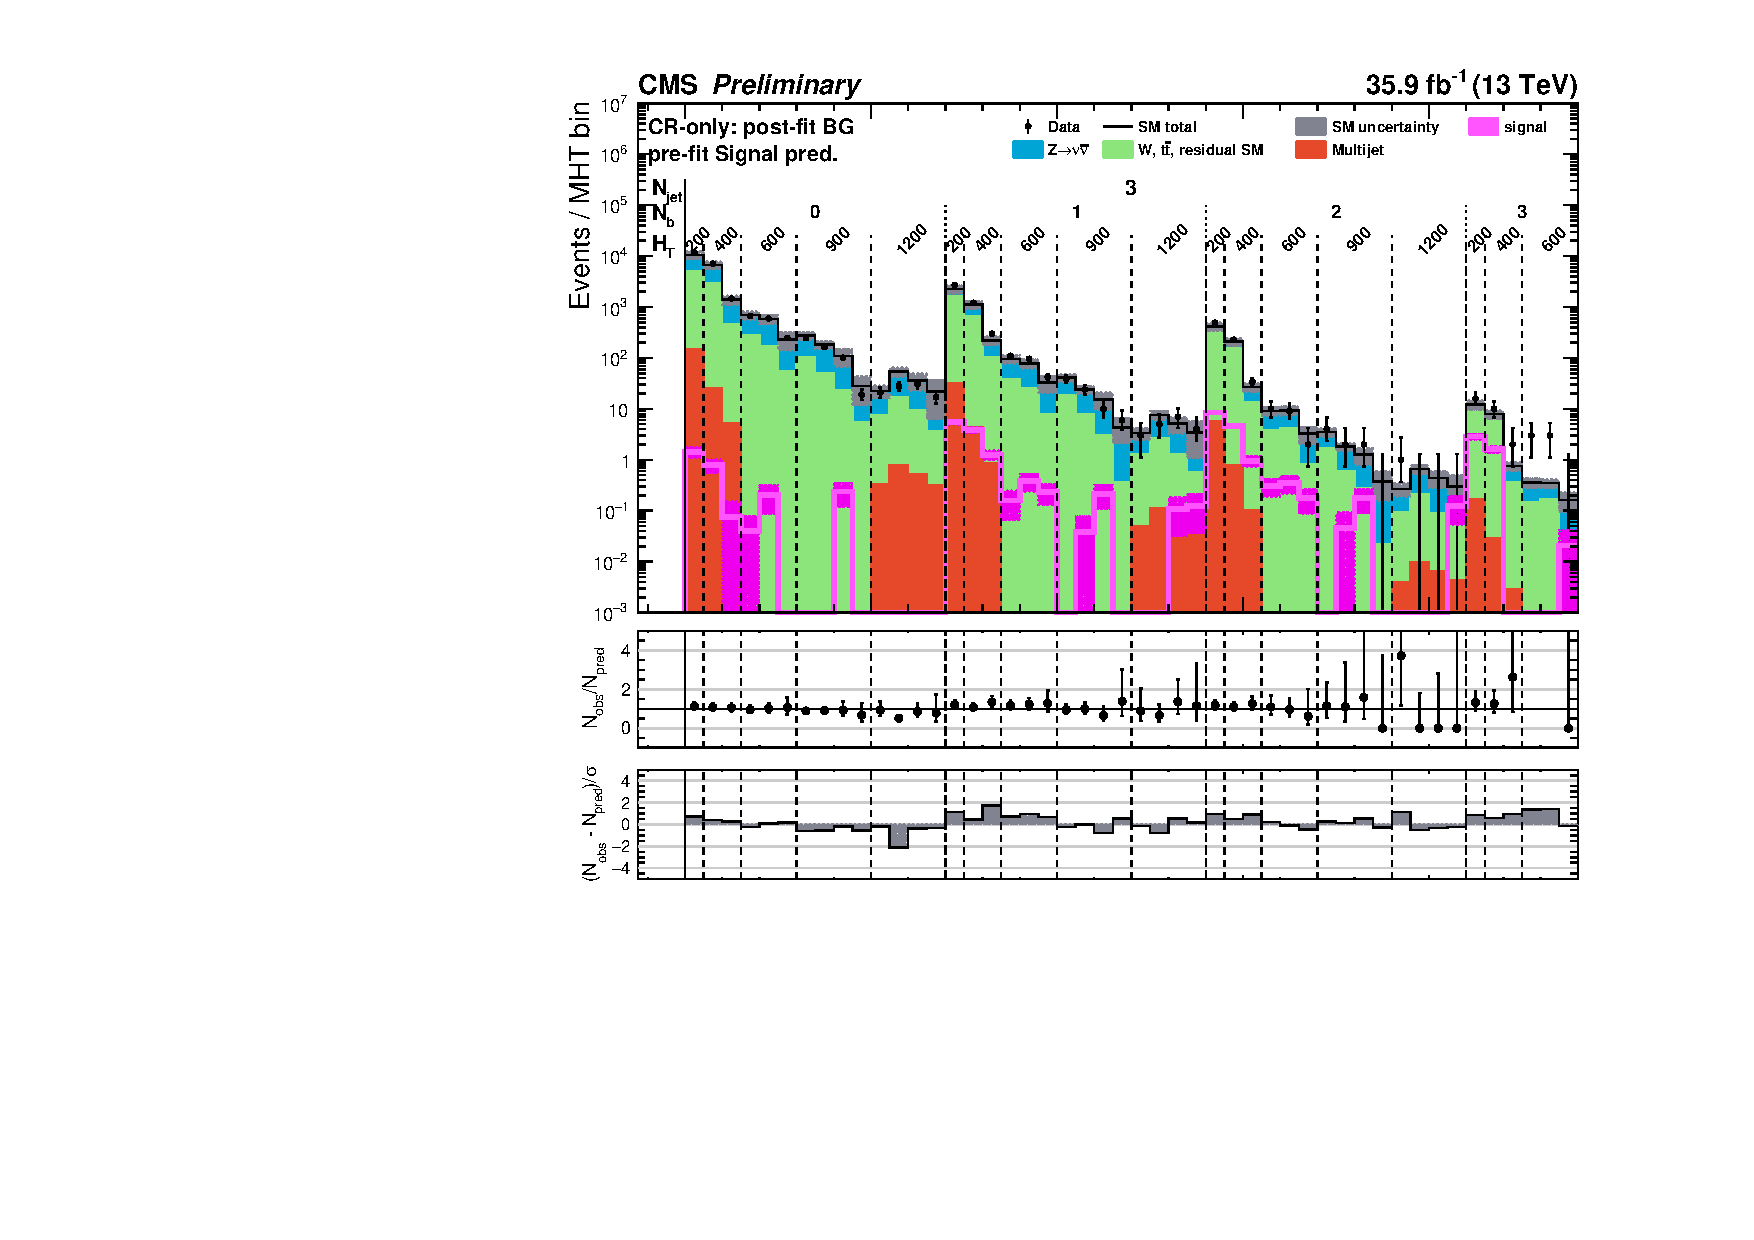
\includegraphics[width=0.49\textwidth]{figures/susyResults/app/T1bbbb_mGluino-1300_mLSP-1100/3jet_full-fit-sig}
%        \label{fig:T1bbbb_compressed_MR_3j}
%    } ~~
%    \subfigure[4 jet]{
%        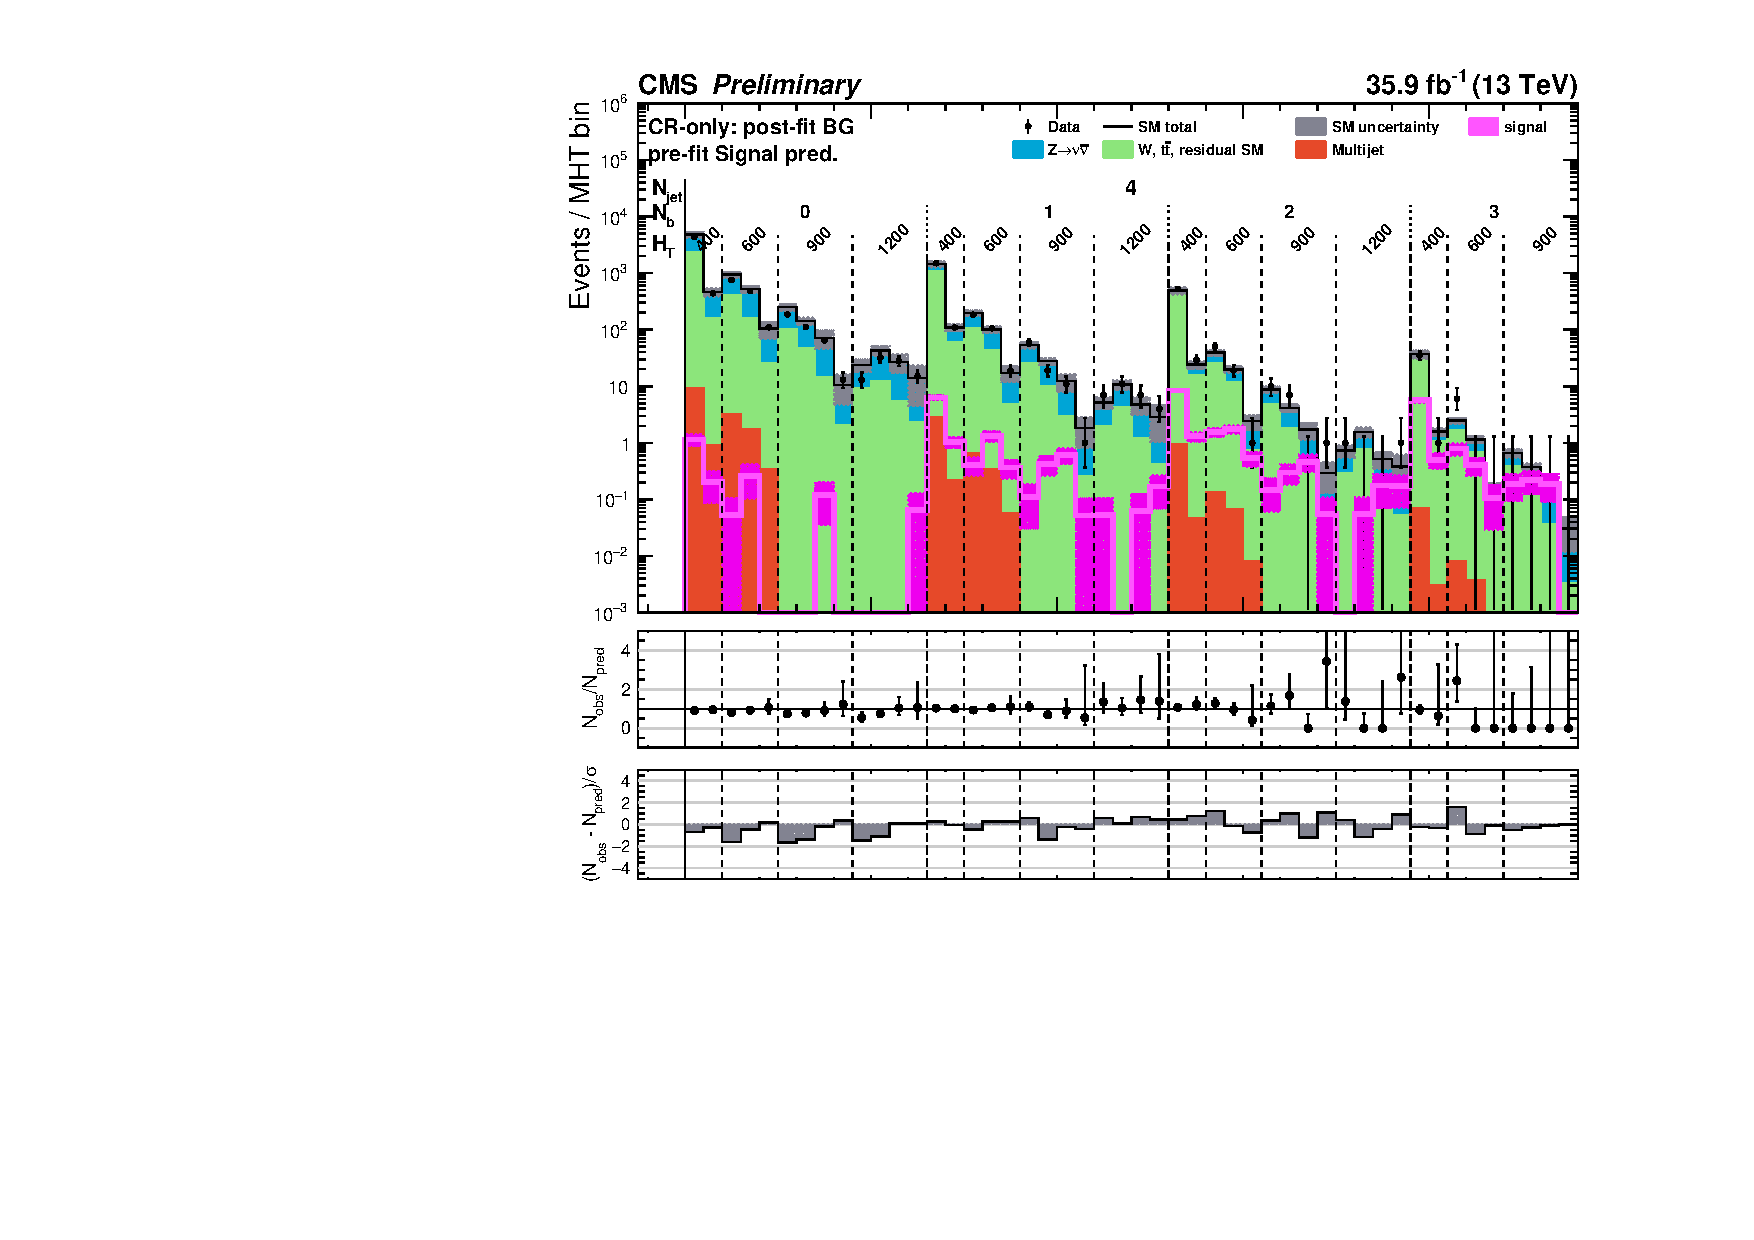
\includegraphics[width=0.49\textwidth]{figures/susyResults/app/T1bbbb_mGluino-1300_mLSP-1100/4jet_full-fit-sig}
%        \label{fig:T1bbbb_compressed_MR_4j}
%    } \\
%    \subfigure[5 jet]{
%        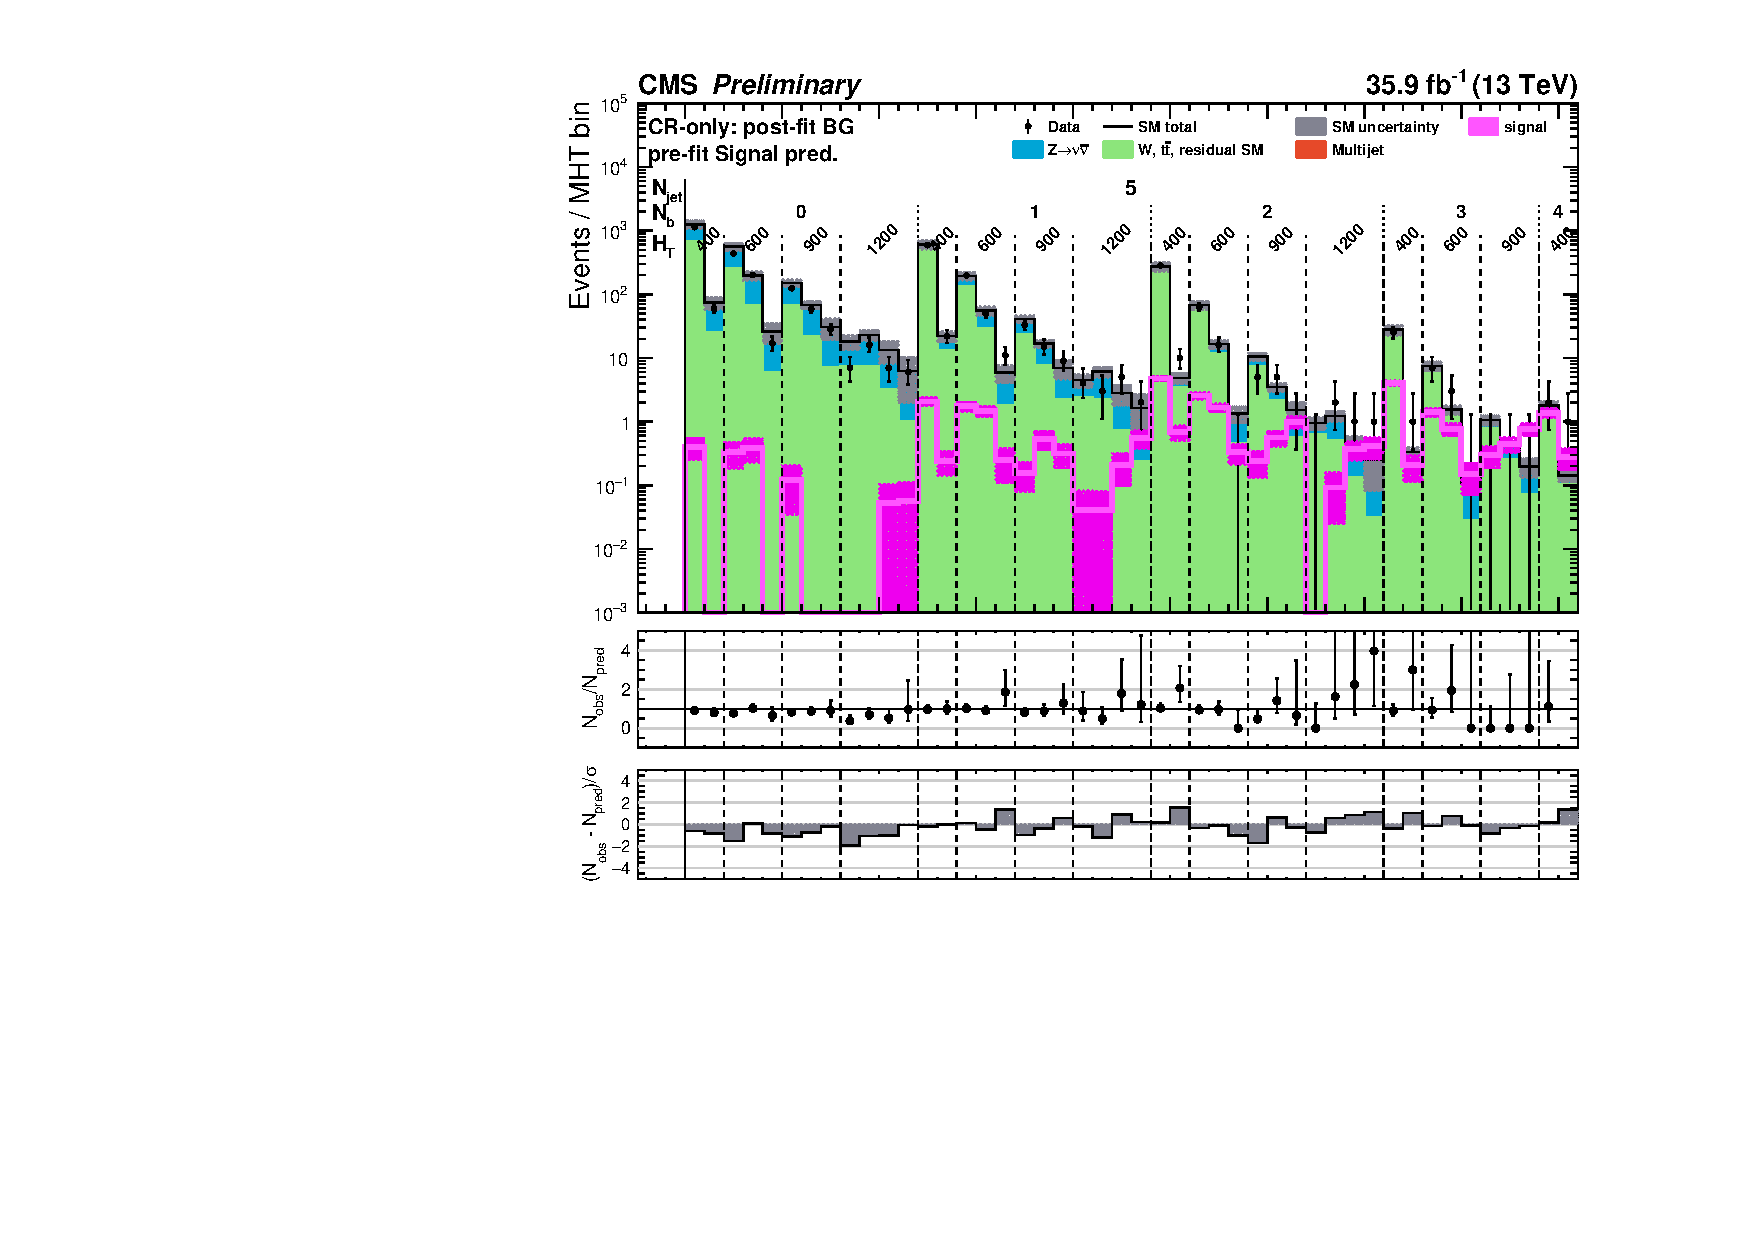
\includegraphics[width=0.49\textwidth]{figures/susyResults/app/T1bbbb_mGluino-1300_mLSP-1100/5jet_full-fit-sig}
%        \label{fig:T1bbbb_compressed_MR_5j}
%    } ~~
%    \subfigure[6+ jet]{
%        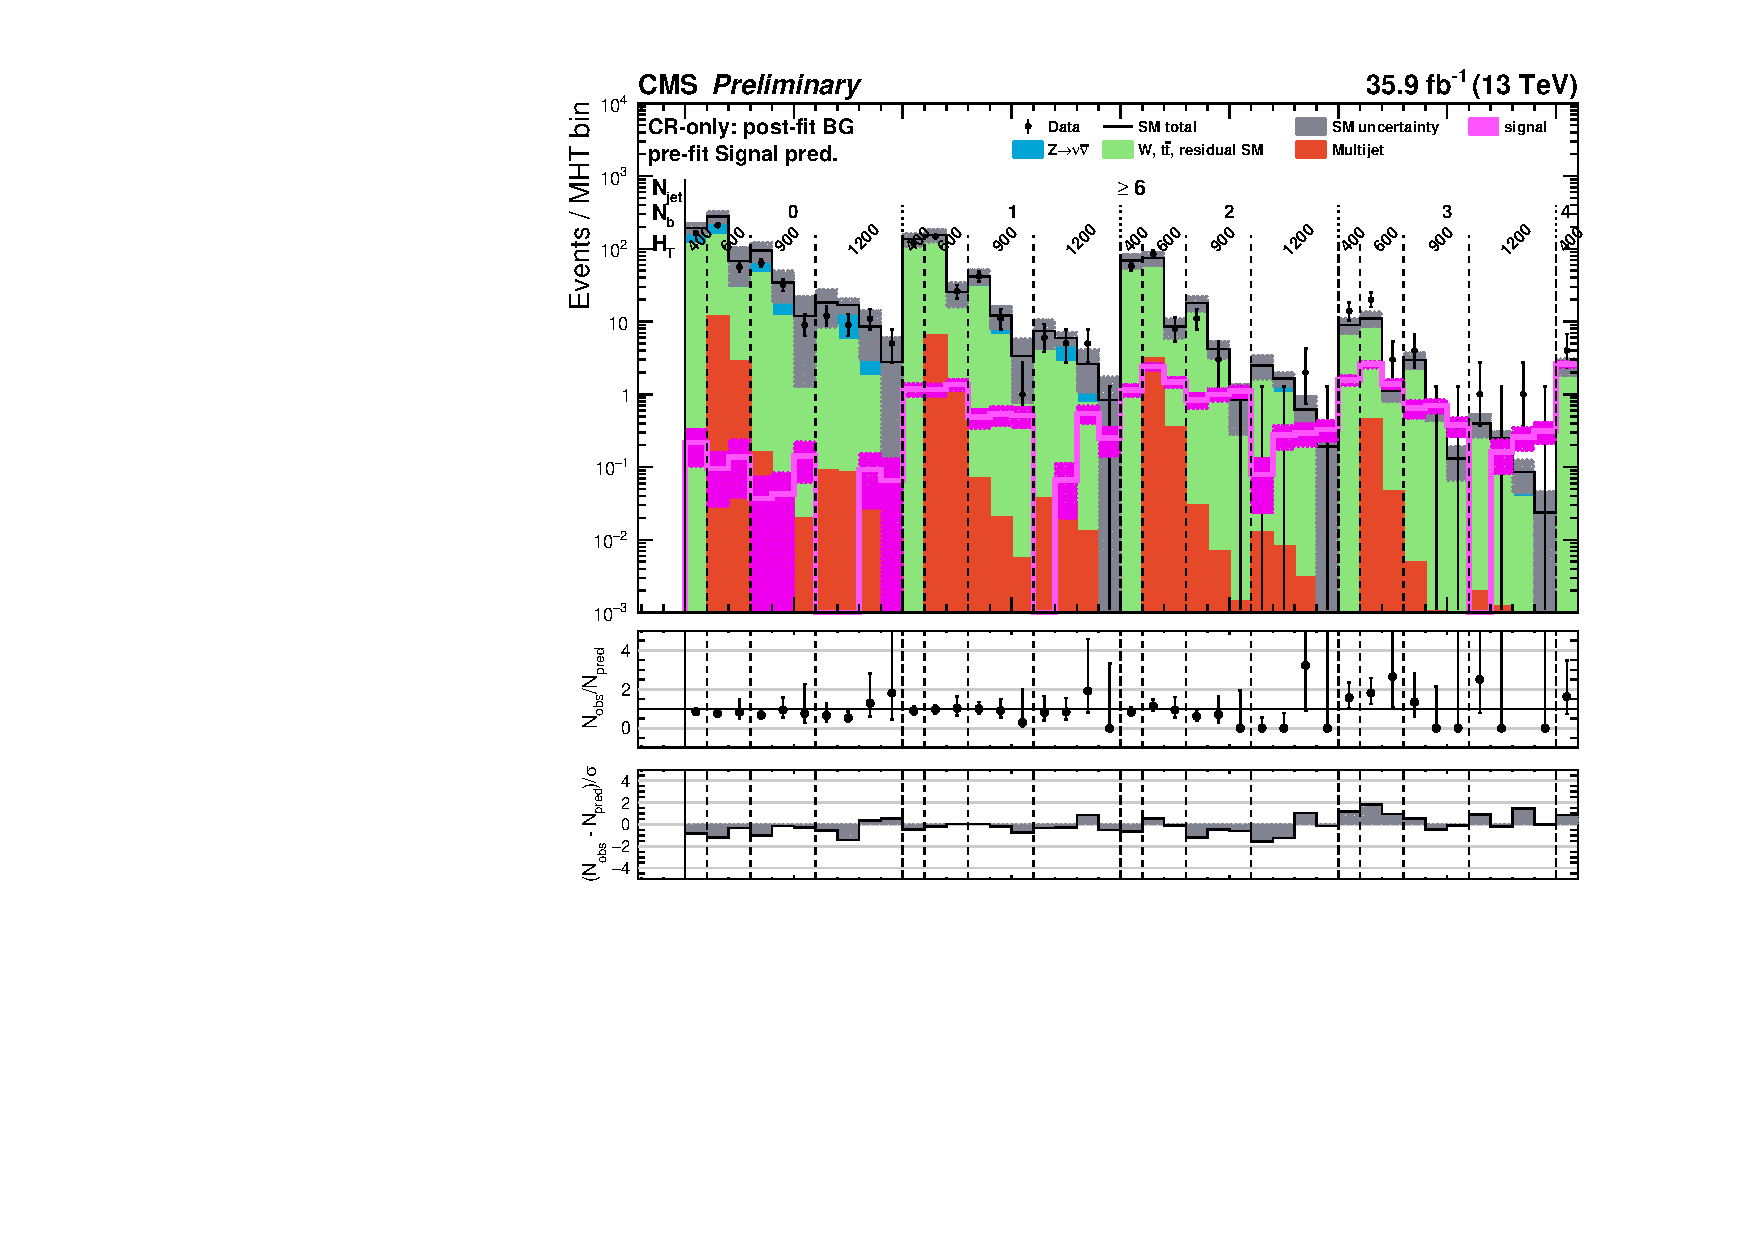
\includegraphics[width=0.49\textwidth]{figures/susyResults/app/T1bbbb_mGluino-1300_mLSP-1100/6+_jets_full-fit-sig}
%        \label{fig:T1bbbb_compressed_MR_6j}
%    } \\
%    \caption{
%        Pre-fit T1bbbb compressed $(1300,1100)$ benchmark model overlay on
%        CR-only post-fit background prediction for all analysis bins. The
%        uncertainty on the signal model counts represents the statistical
%        uncertainty due to the finite size of the of the simulated sample.
%    }
%    \label{fig:T1bbbb_compressed_MR}
%\end{figure}
%
%\begin{figure}[!h]
%    \centering
%    \subfigure[Monojet]{
%        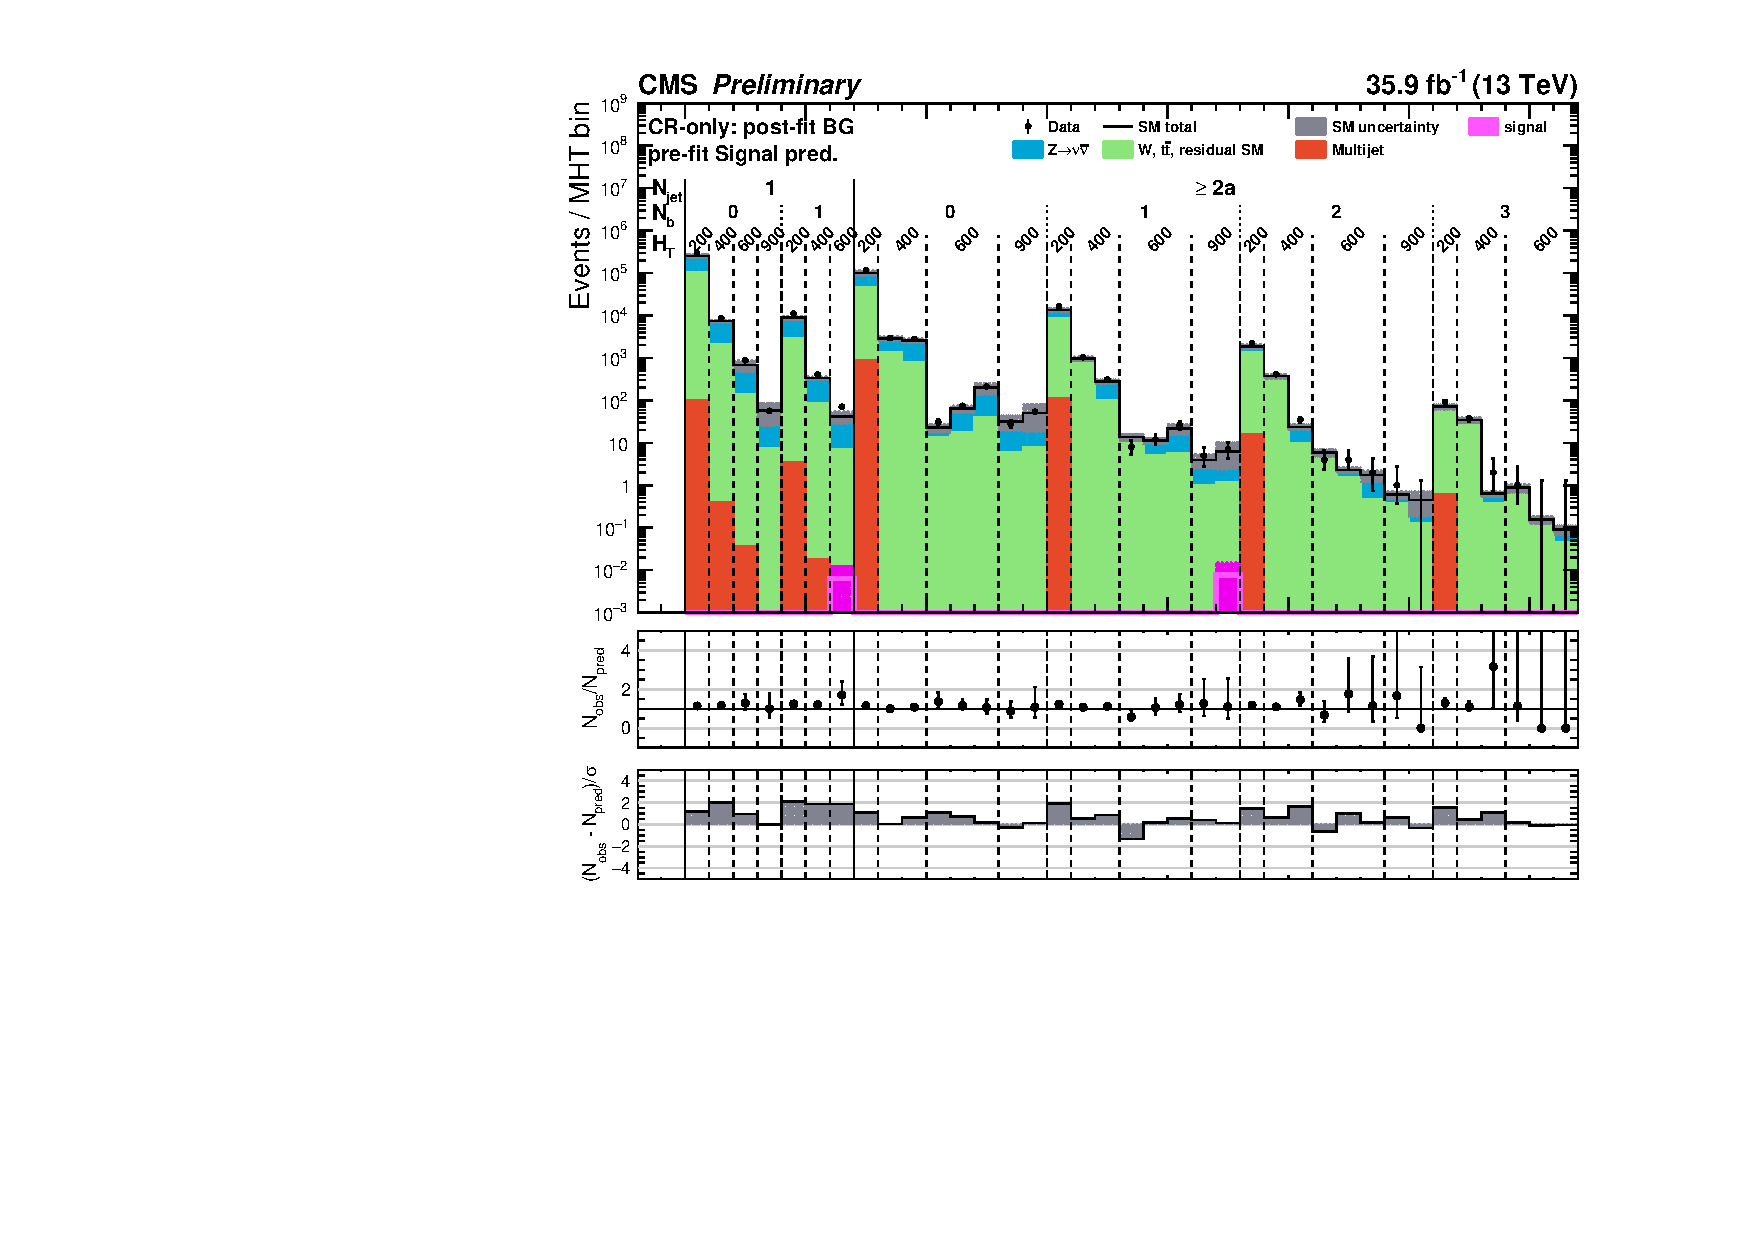
\includegraphics[width=0.49\textwidth]{figures/susyResults/app/T1bbbb_mGluino-1900_mLSP-100/monojet_full-fit-sig}
%        \label{fig:T1bbbb_uncompressed_MR_1j}
%    } ~~
%    \subfigure[Di-jet]{
%        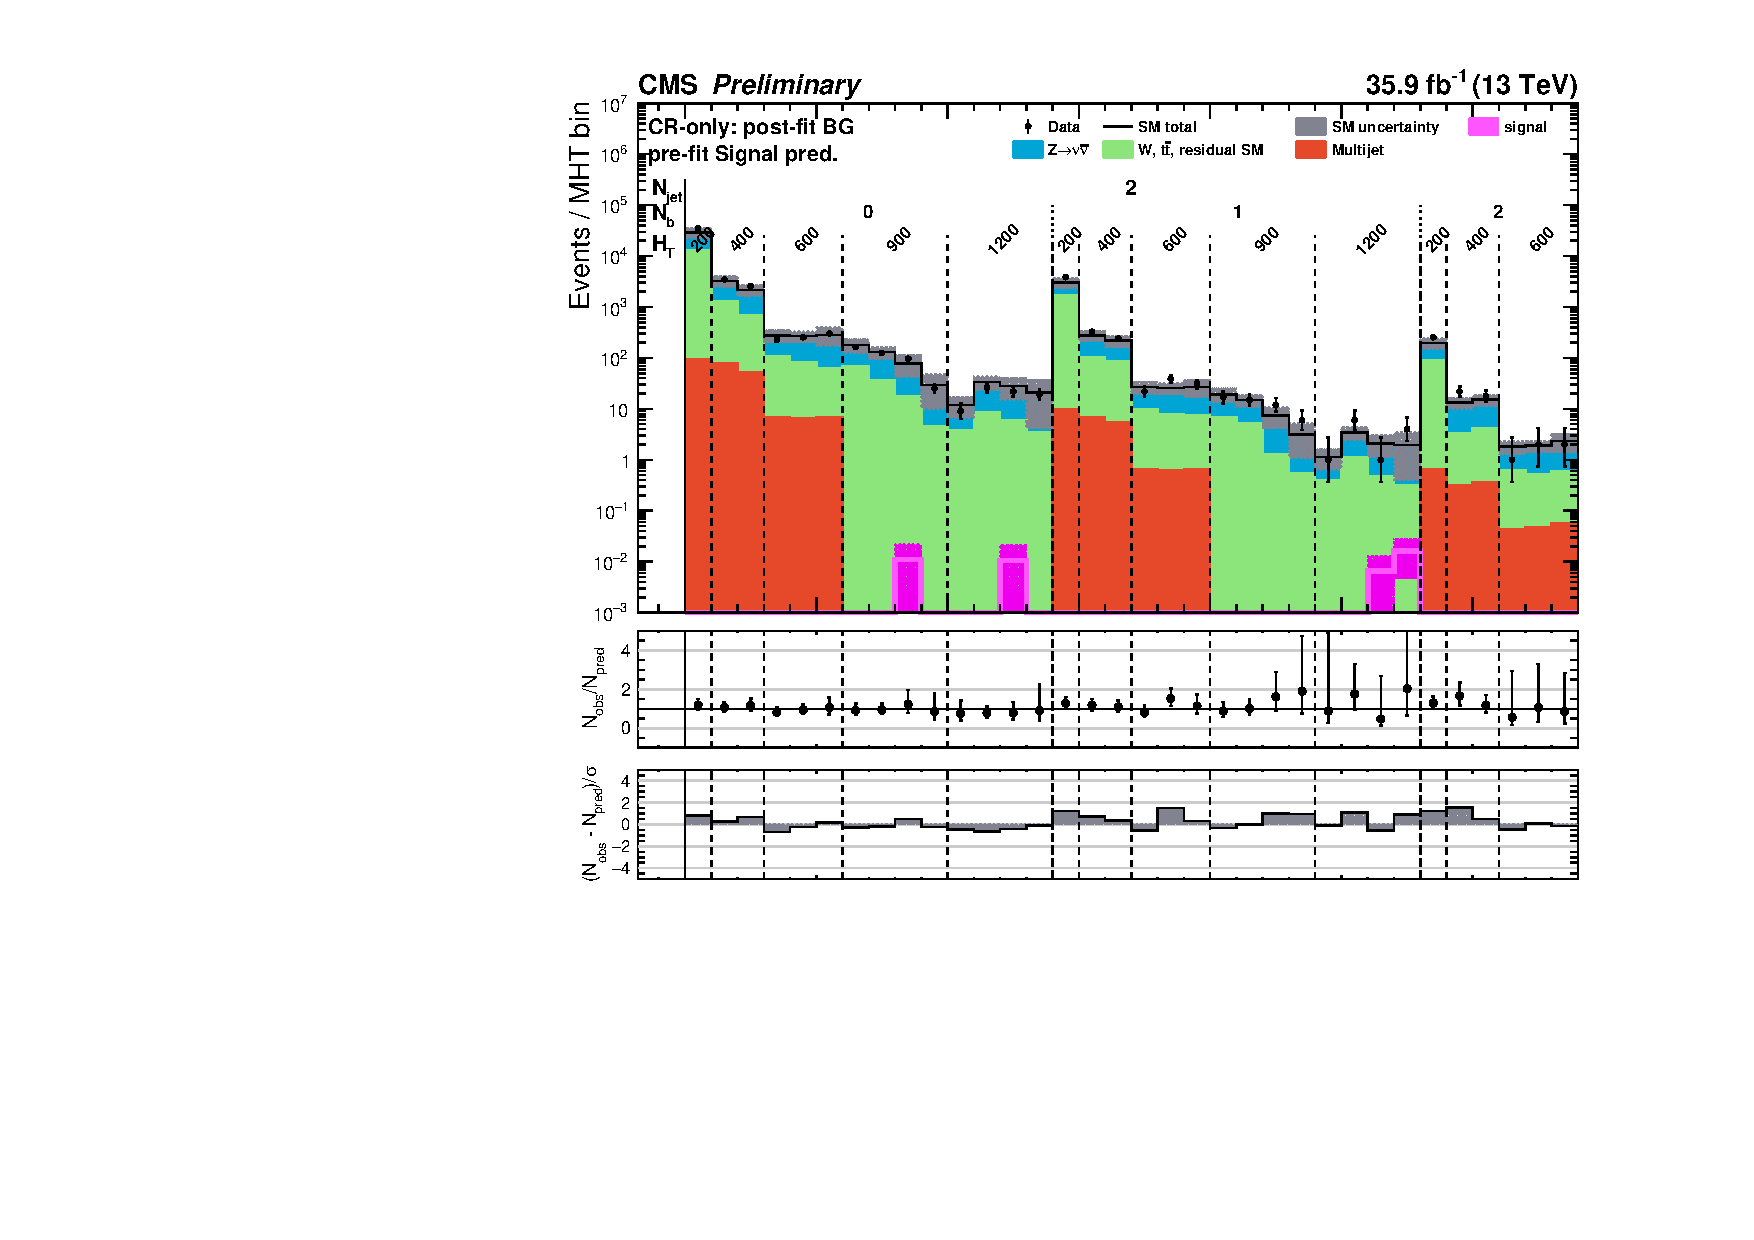
\includegraphics[width=0.49\textwidth]{figures/susyResults/app/T1bbbb_mGluino-1900_mLSP-100/di-jet_full-fit-sig}
%        \label{fig:T1bbbb_uncompressed_MR_2j}
%    } \\
%    \subfigure[3 jet]{
%        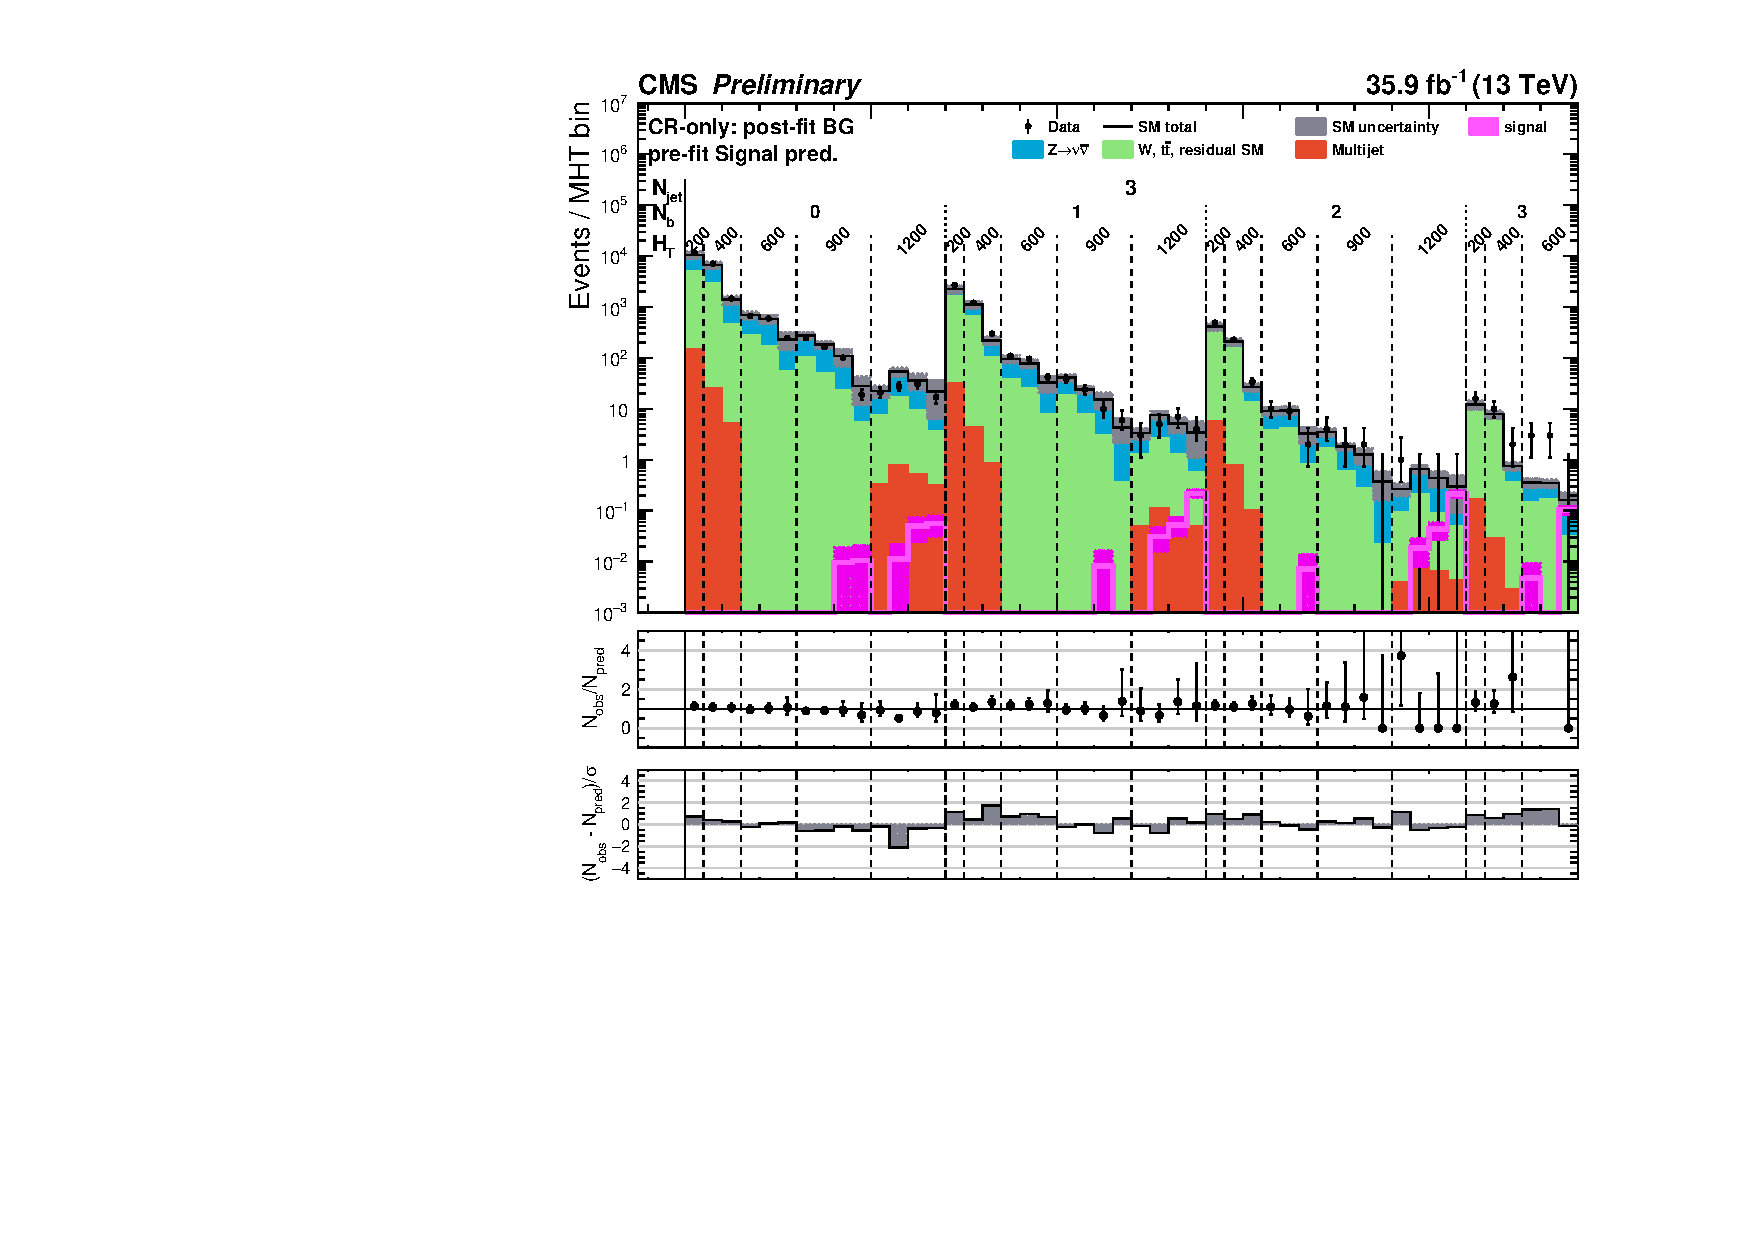
\includegraphics[width=0.49\textwidth]{figures/susyResults/app/T1bbbb_mGluino-1900_mLSP-100/3jet_full-fit-sig}
%        \label{fig:T1bbbb_uncompressed_MR_3j}
%    } ~~
%    \subfigure[4 jet]{
%        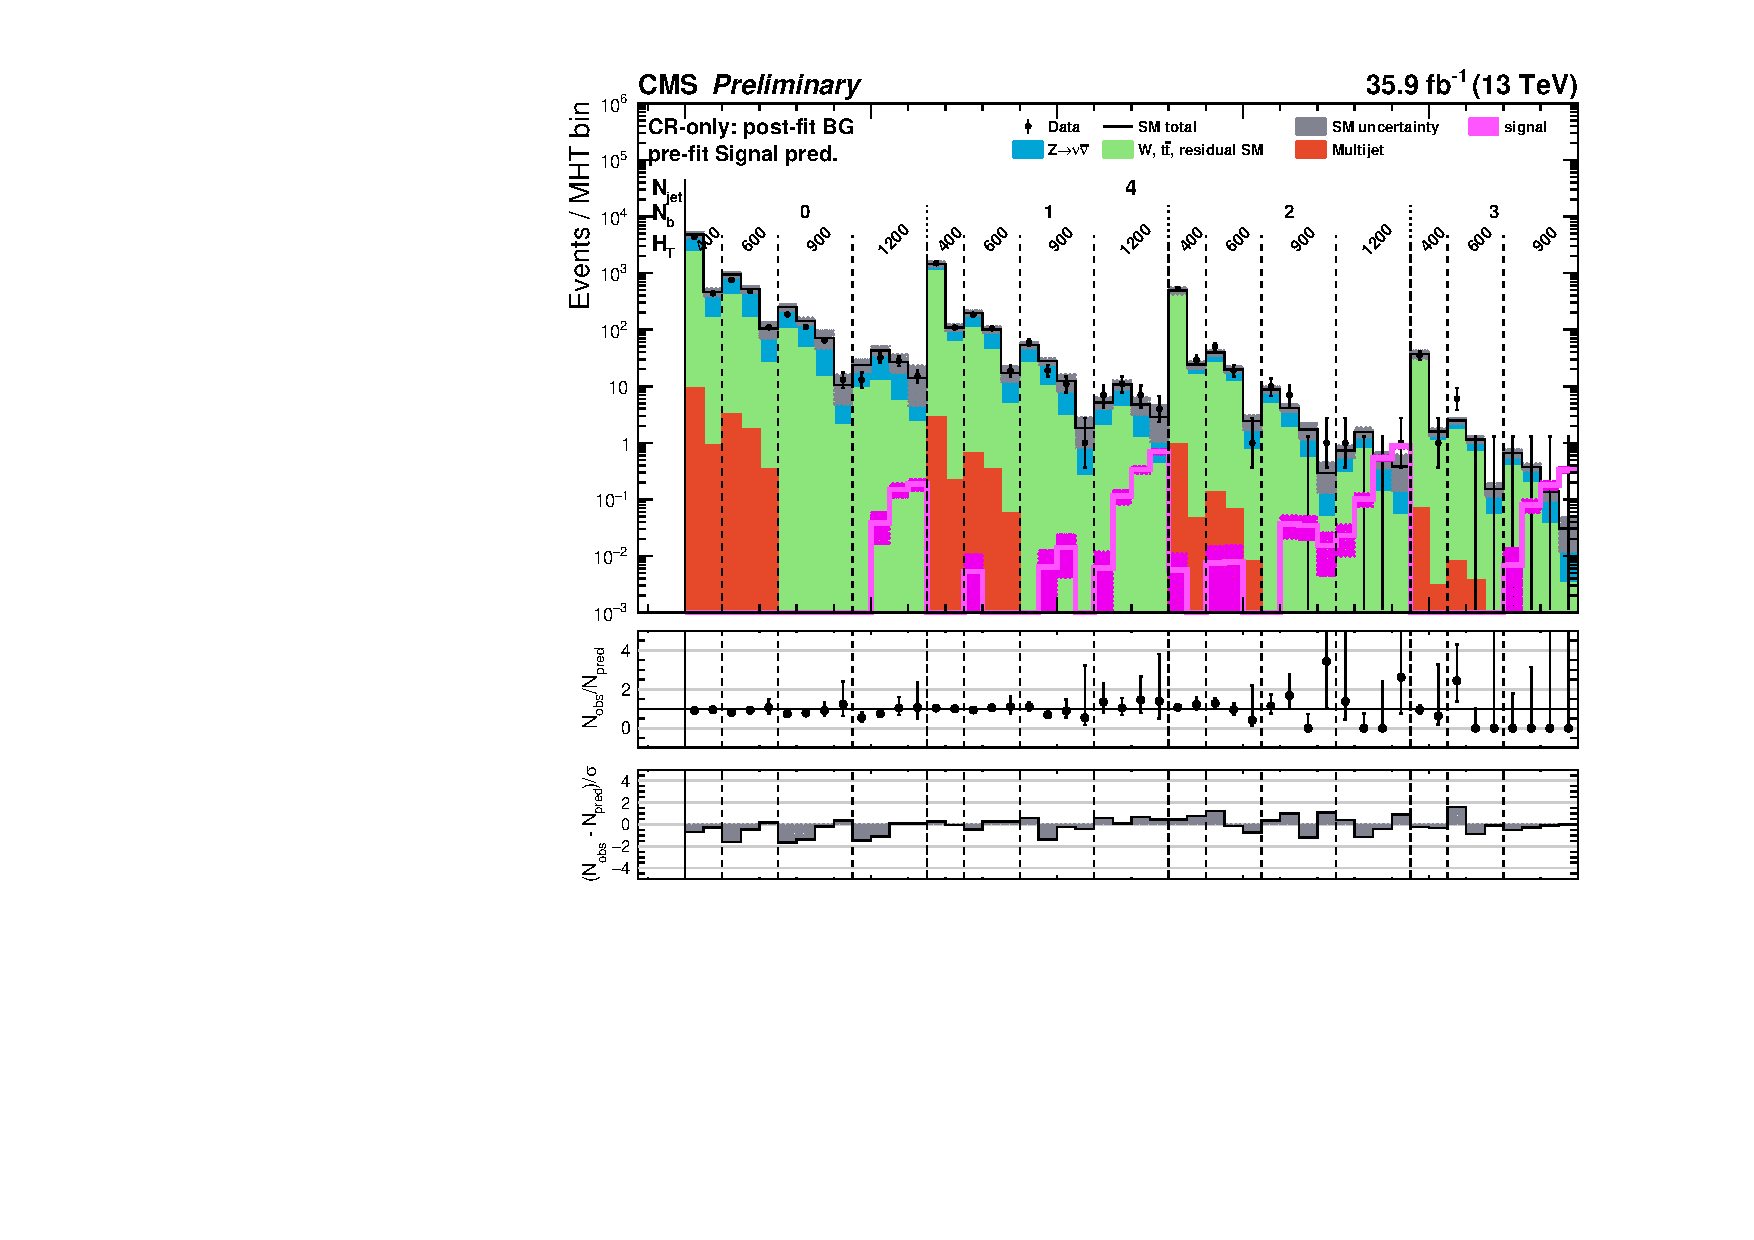
\includegraphics[width=0.49\textwidth]{figures/susyResults/app/T1bbbb_mGluino-1900_mLSP-100/4jet_full-fit-sig}
%        \label{fig:T1bbbb_uncompressed_MR_4j}
%    } \\
%    \subfigure[5 jet]{
%        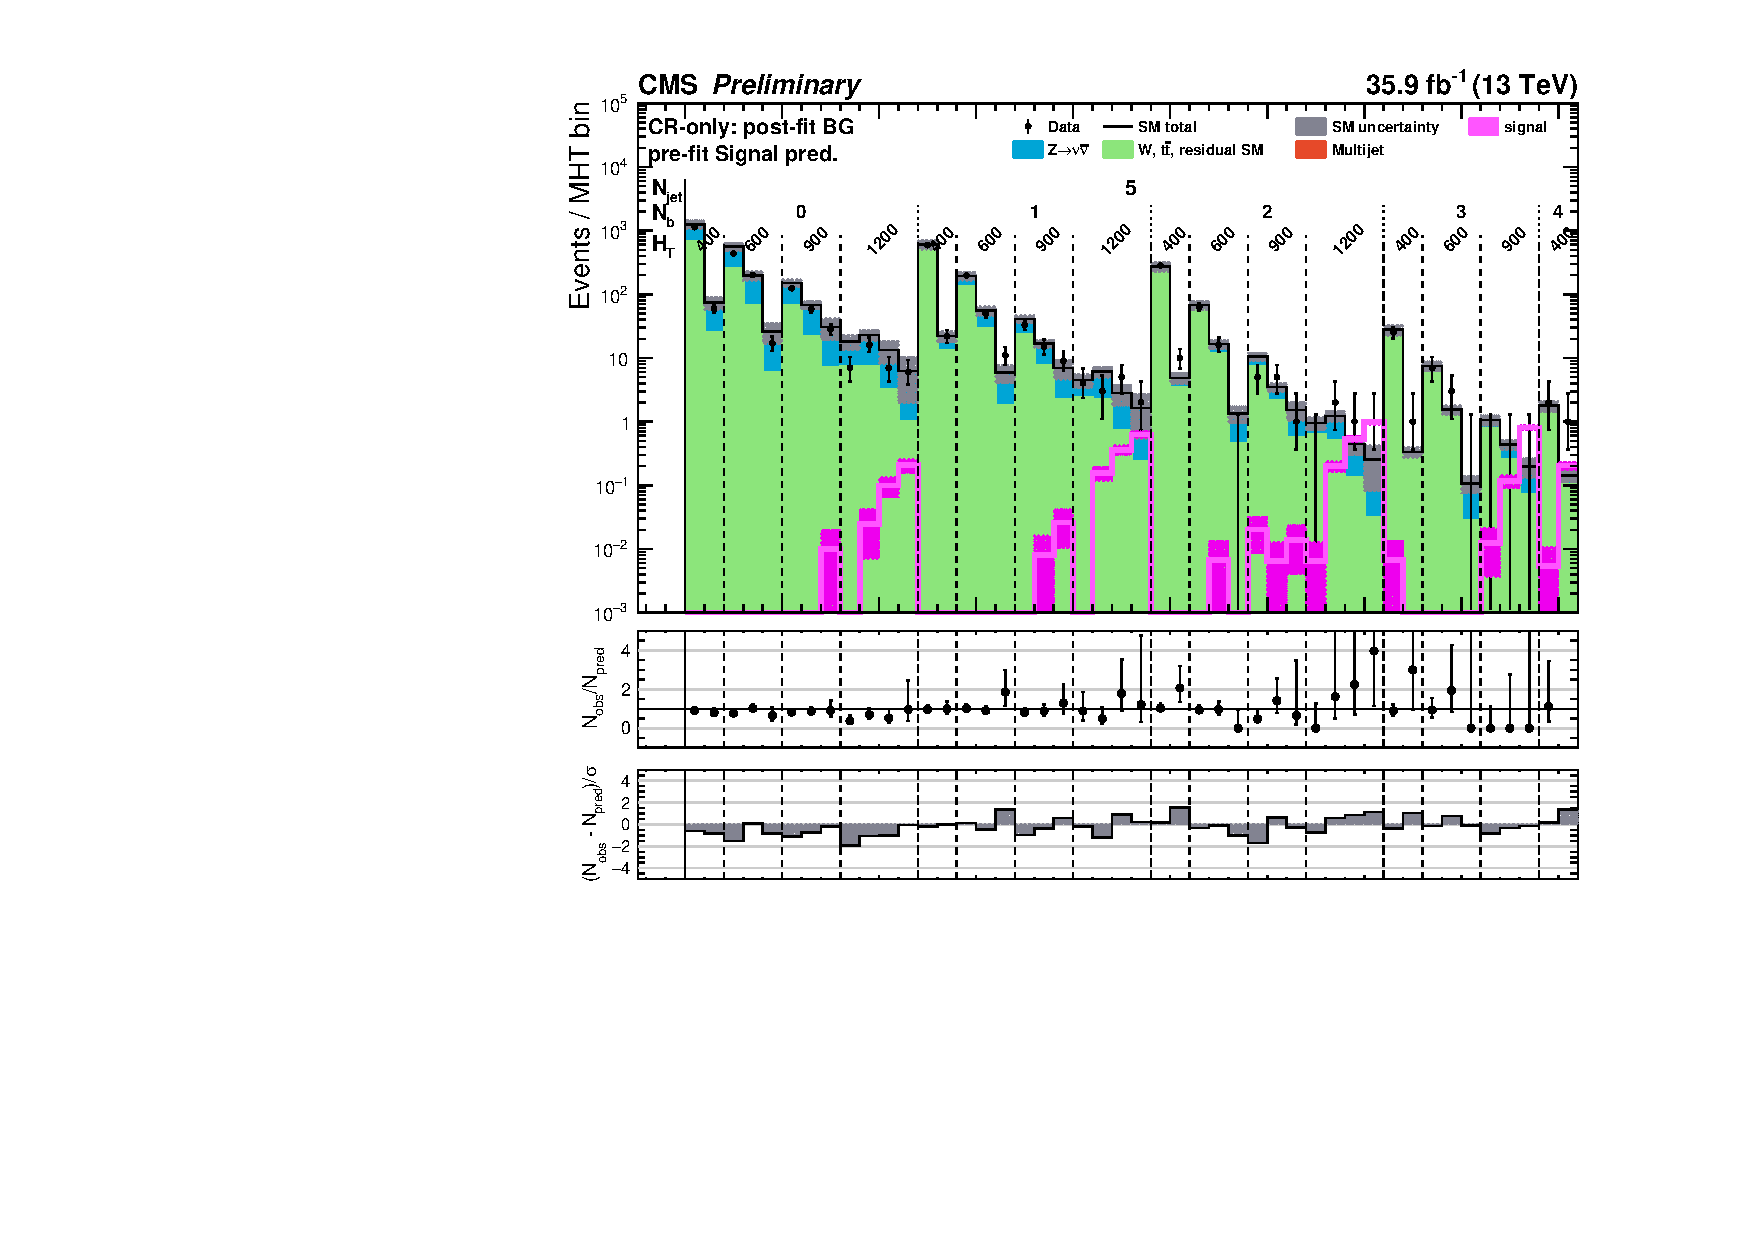
\includegraphics[width=0.49\textwidth]{figures/susyResults/app/T1bbbb_mGluino-1900_mLSP-100/5jet_full-fit-sig}
%        \label{fig:T1bbbb_uncompressed_MR_5j}
%    } ~~
%    \subfigure[6+ jet]{
%        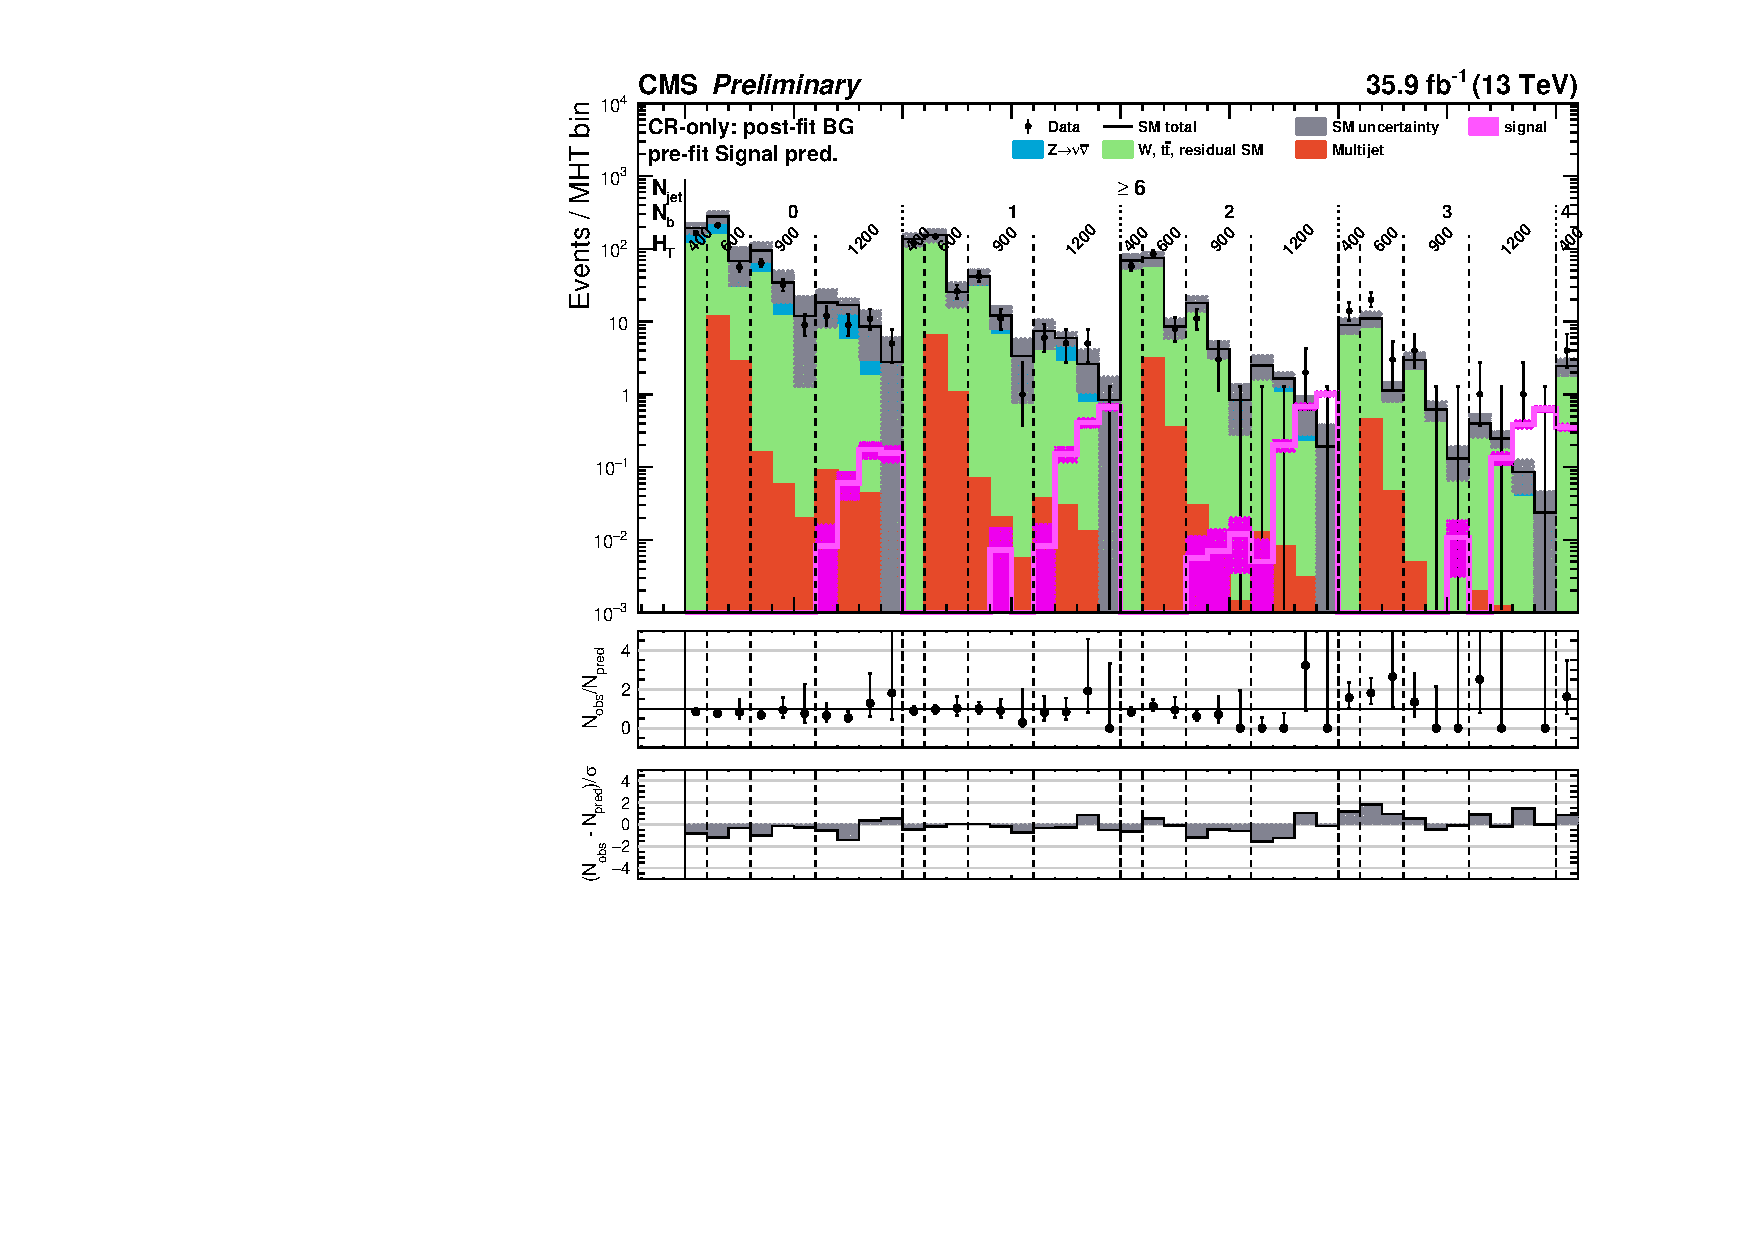
\includegraphics[width=0.49\textwidth]{figures/susyResults/app/T1bbbb_mGluino-1900_mLSP-100/6+_jets_full-fit-sig}
%        \label{fig:T1bbbb_uncompressed_MR_6j}
%    } \\
%    \caption{
%        Pre-fit T1bbbb uncompressed $(1900,100)$ benchmark model overlay on
%        CR-only post-fit background prediction for all analysis bins. The
%        uncertainty on the signal model counts represents the statistical
%        uncertainty due to the finite size of the of the simulated sample.
%    }
%    \label{fig:T1bbbb_uncompressed_MR}
%\end{figure}
%
%\begin{figure}[!h]
%    \centering
%    \subfigure[Monojet]{
%        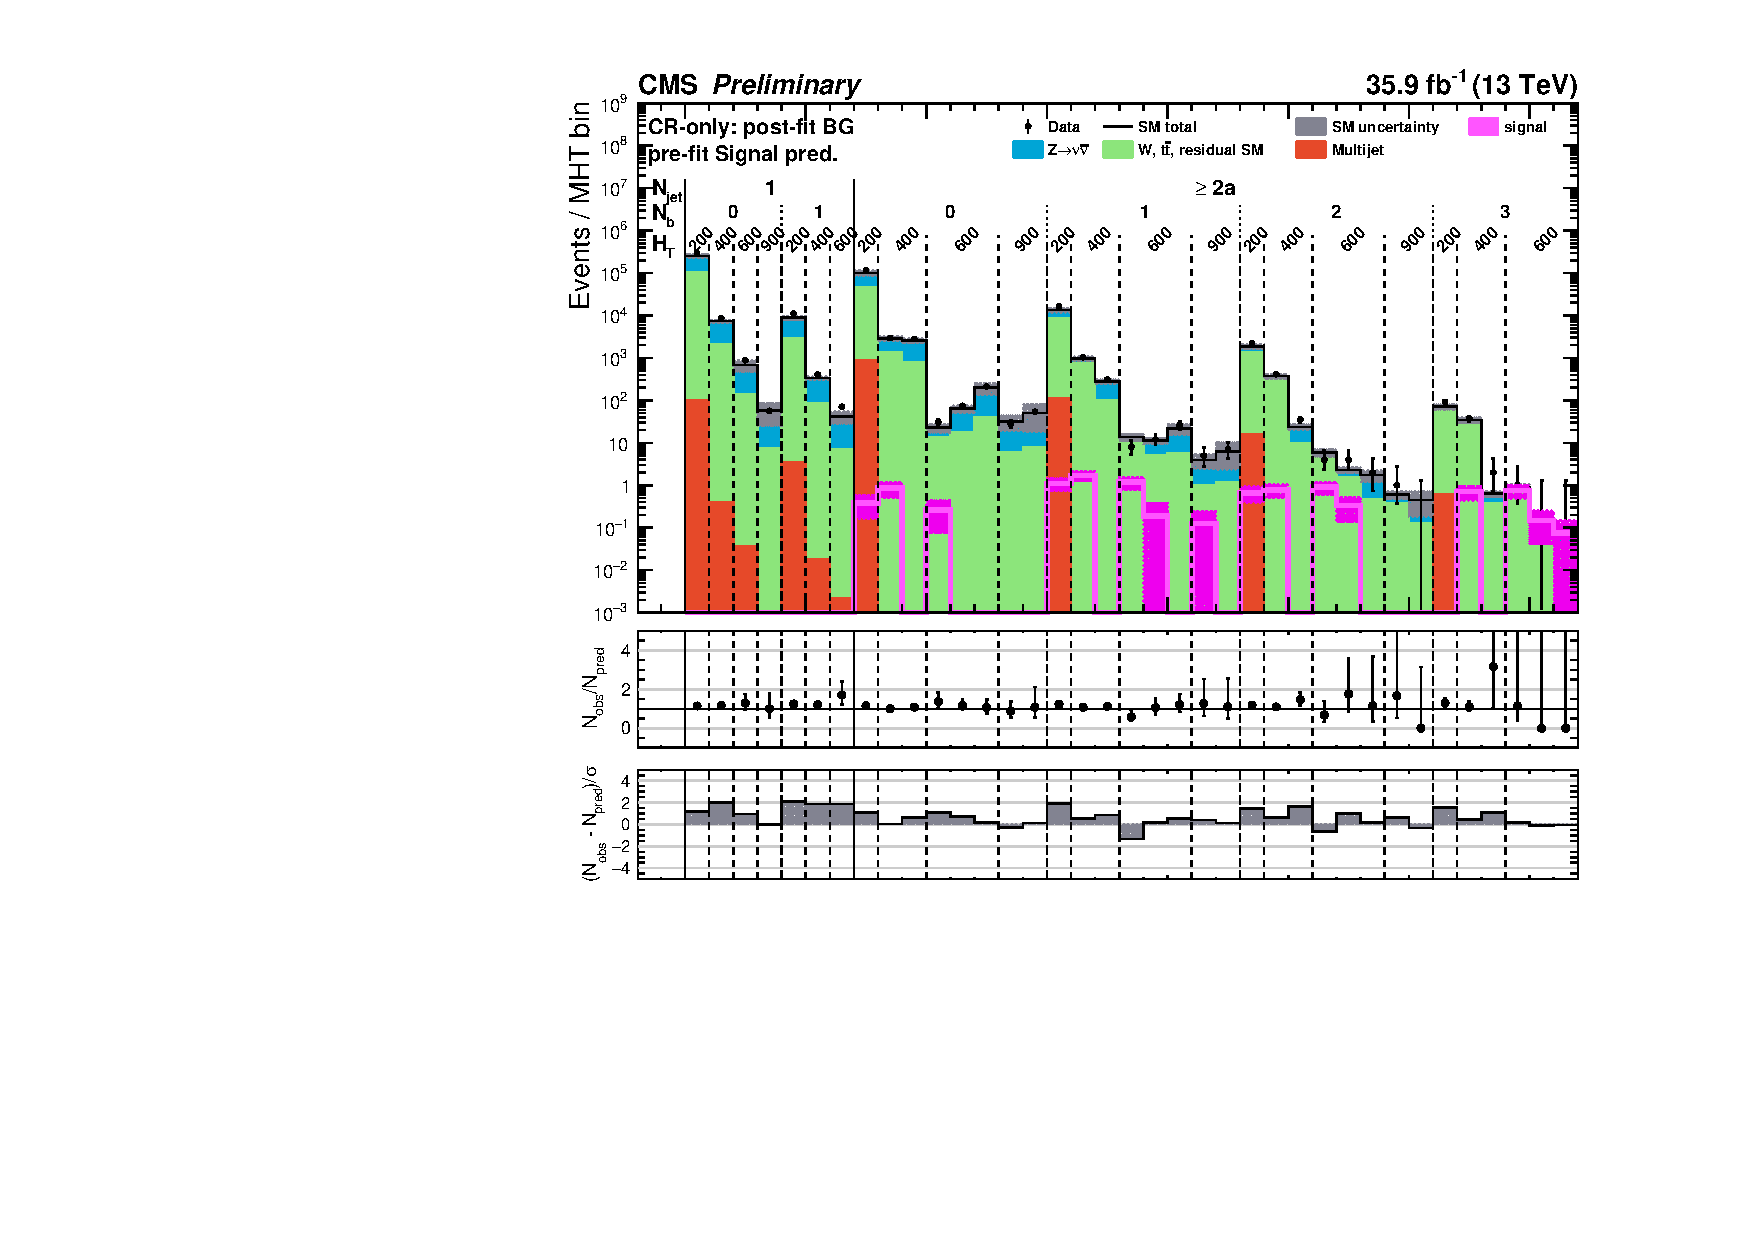
\includegraphics[width=0.49\textwidth]{figures/susyResults/app/T1tttt_mGluino-950_mLSP-600/monojet_full-fit-sig}
%        \label{fig:T1tttt_compressed_MR_1j}
%    } ~~
%    \subfigure[Di-jet]{
%        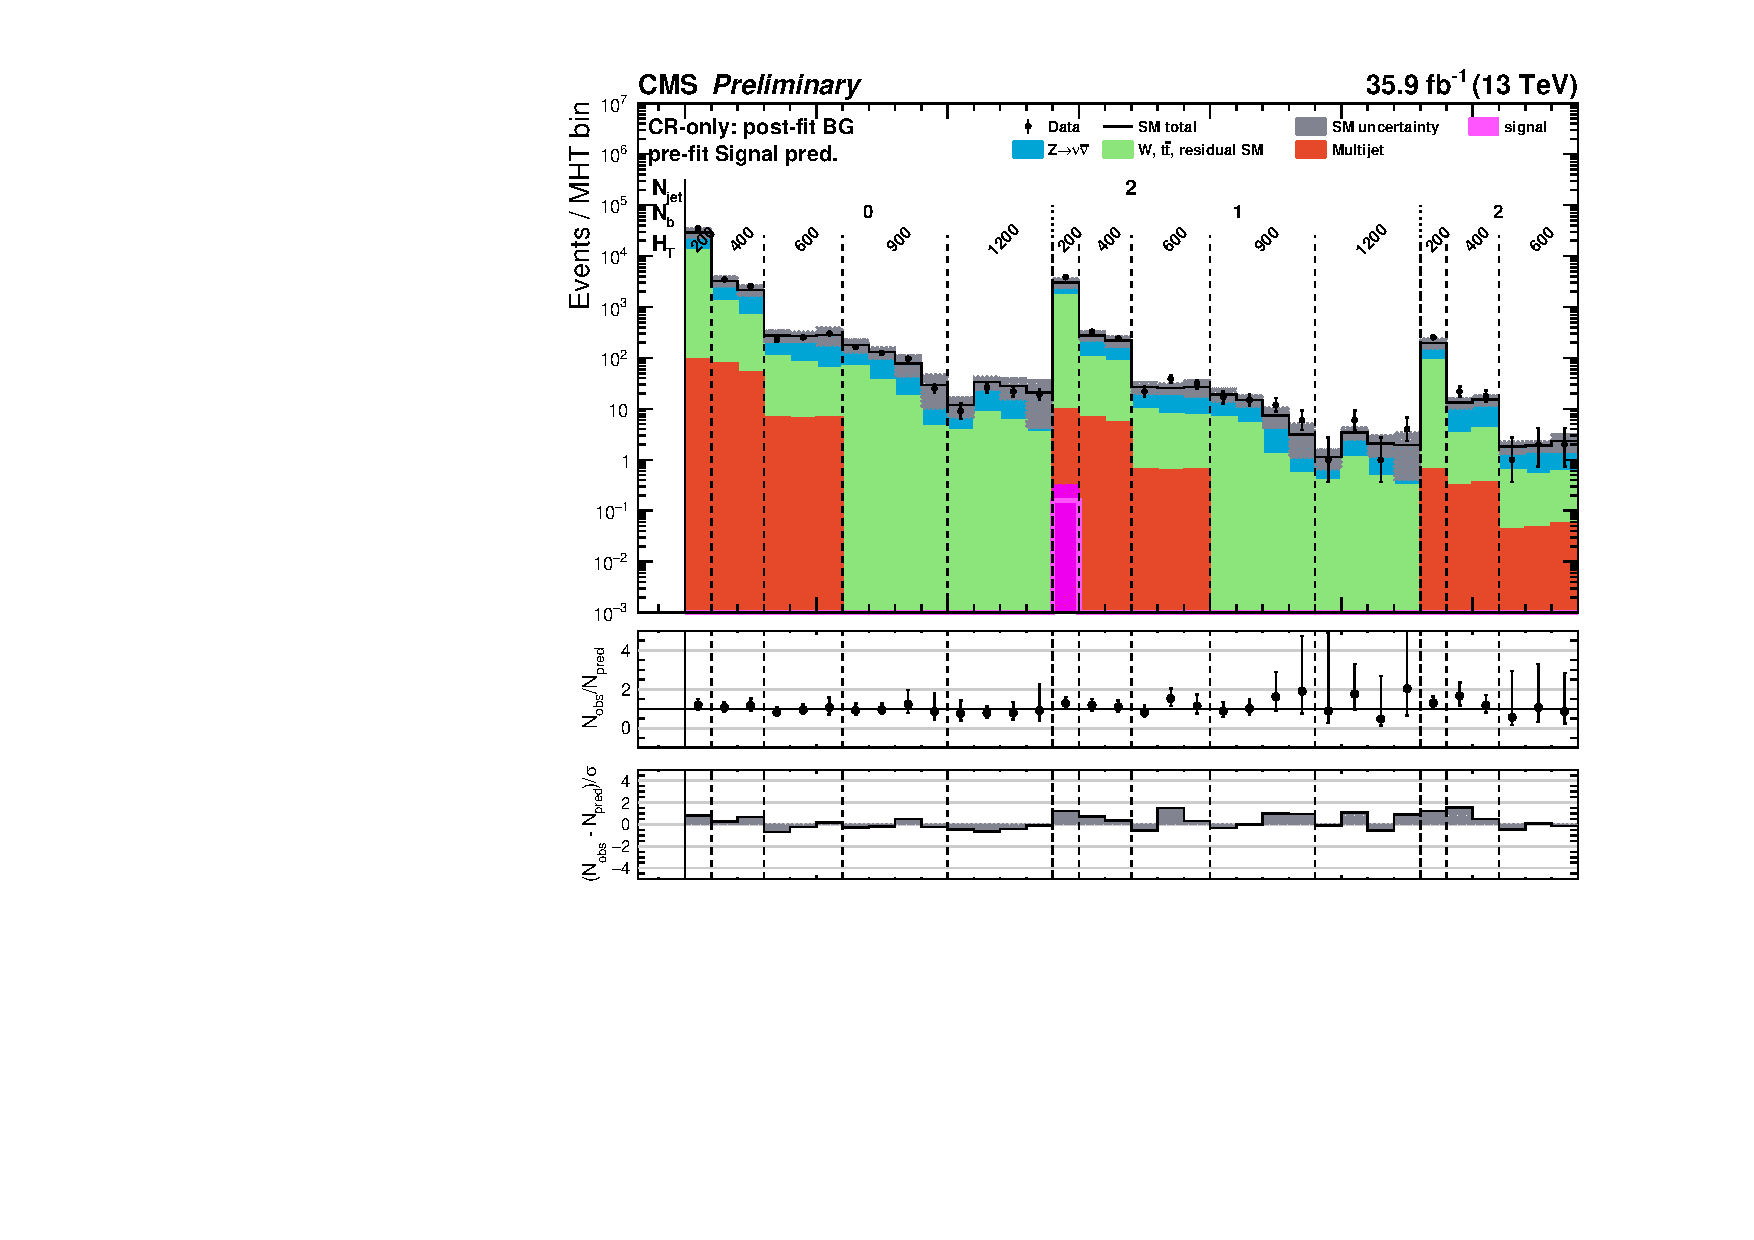
\includegraphics[width=0.49\textwidth]{figures/susyResults/app/T1tttt_mGluino-950_mLSP-600/di-jet_full-fit-sig}
%        \label{fig:T1tttt_compressed_MR_2j}
%    } \\
%    \subfigure[3 jet]{
%        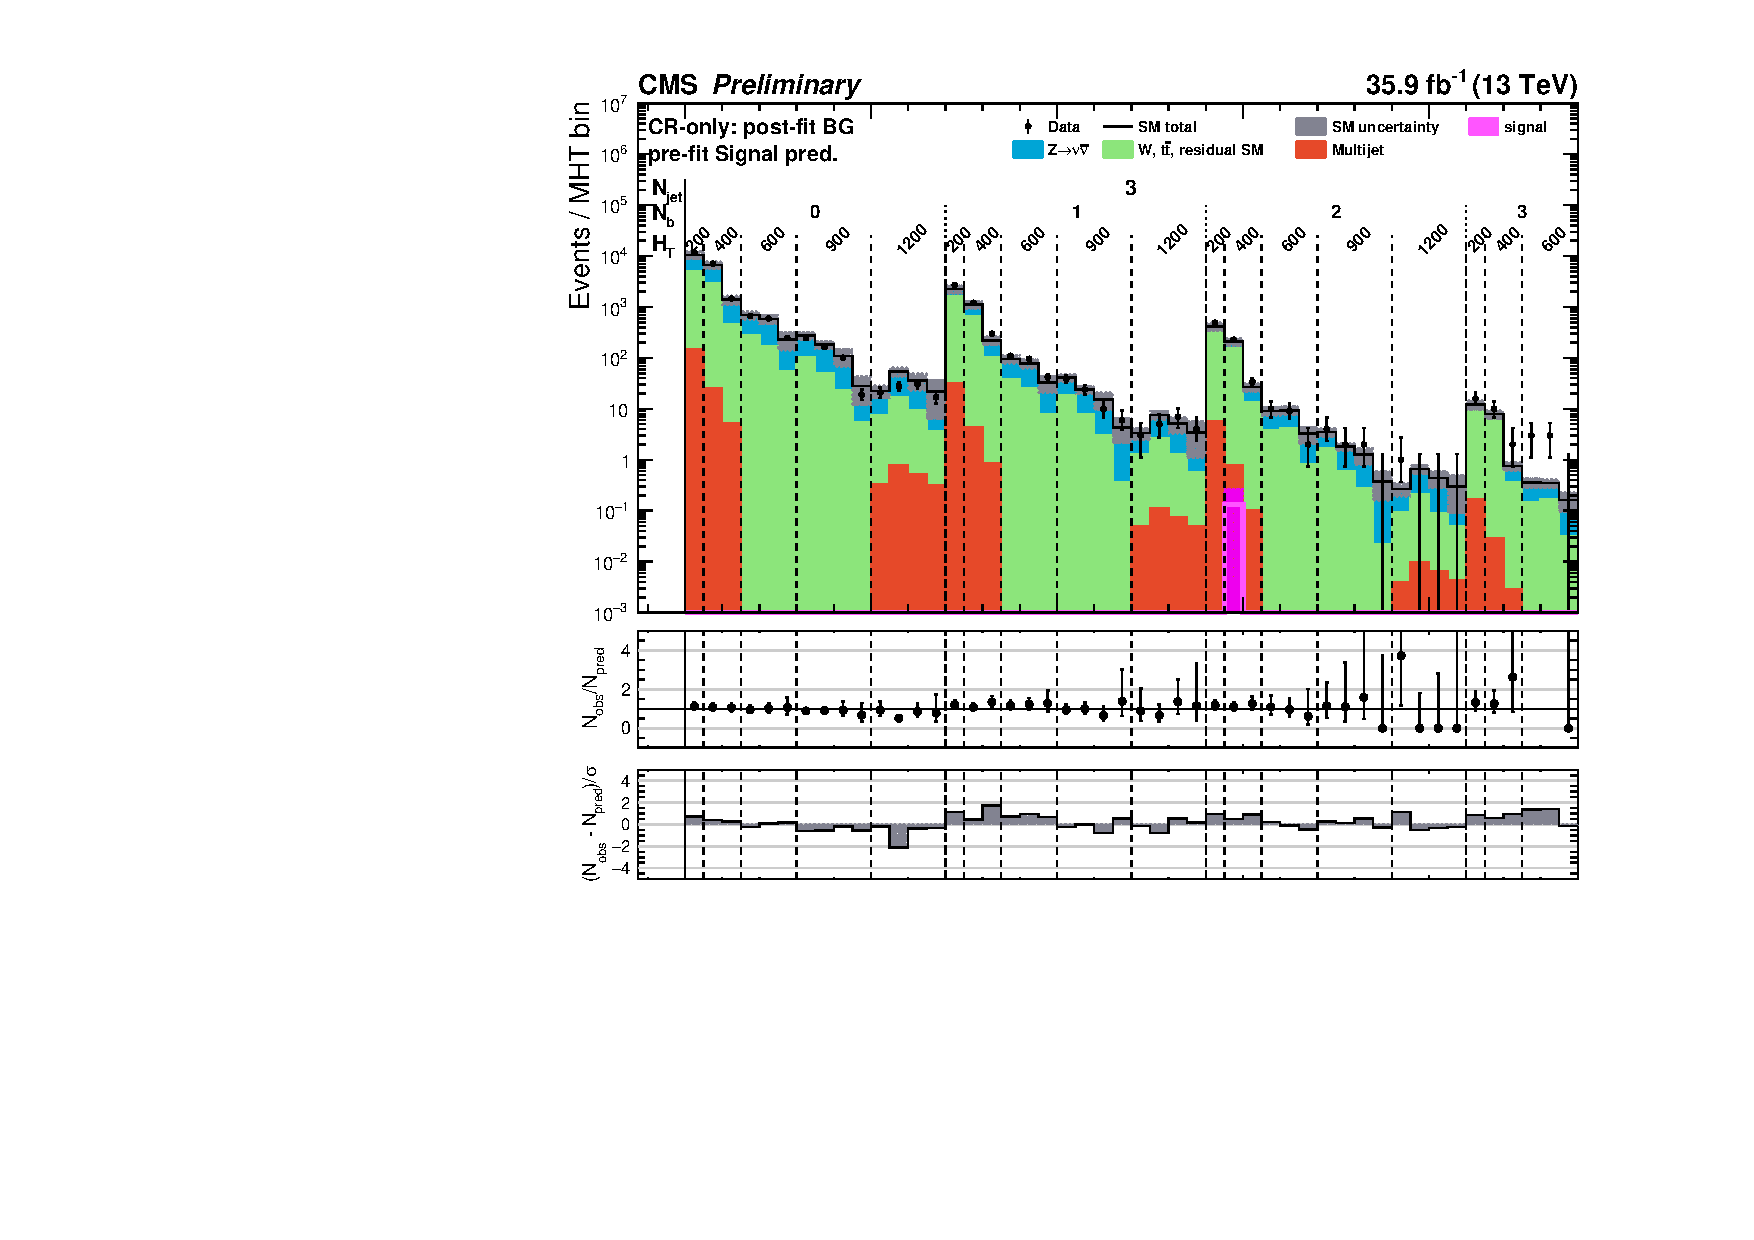
\includegraphics[width=0.49\textwidth]{figures/susyResults/app/T1tttt_mGluino-950_mLSP-600/3jet_full-fit-sig}
%        \label{fig:T1tttt_compressed_MR_3j}
%    } ~~
%    \subfigure[4 jet]{
%        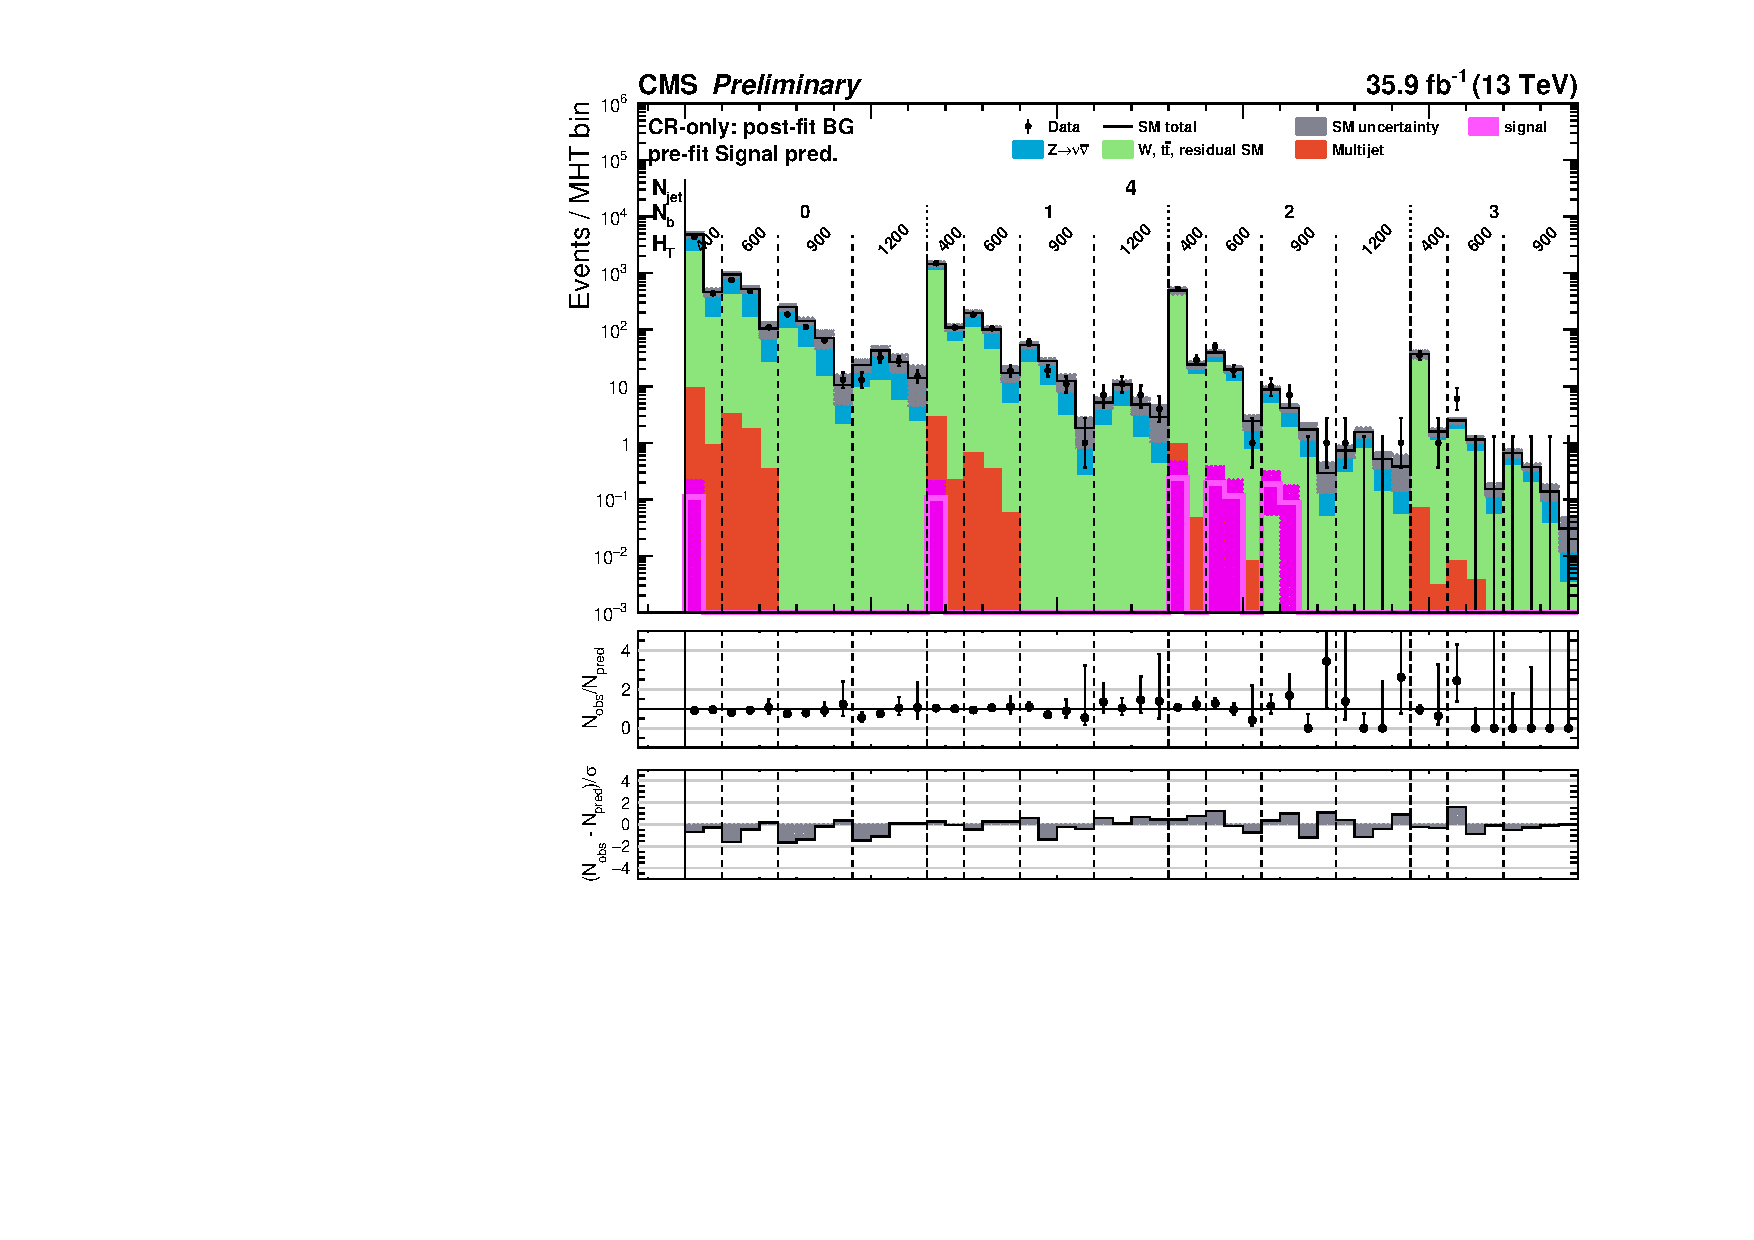
\includegraphics[width=0.49\textwidth]{figures/susyResults/app/T1tttt_mGluino-950_mLSP-600/4jet_full-fit-sig}
%        \label{fig:T1tttt_compressed_MR_4j}
%    } \\
%    \subfigure[5 jet]{
%        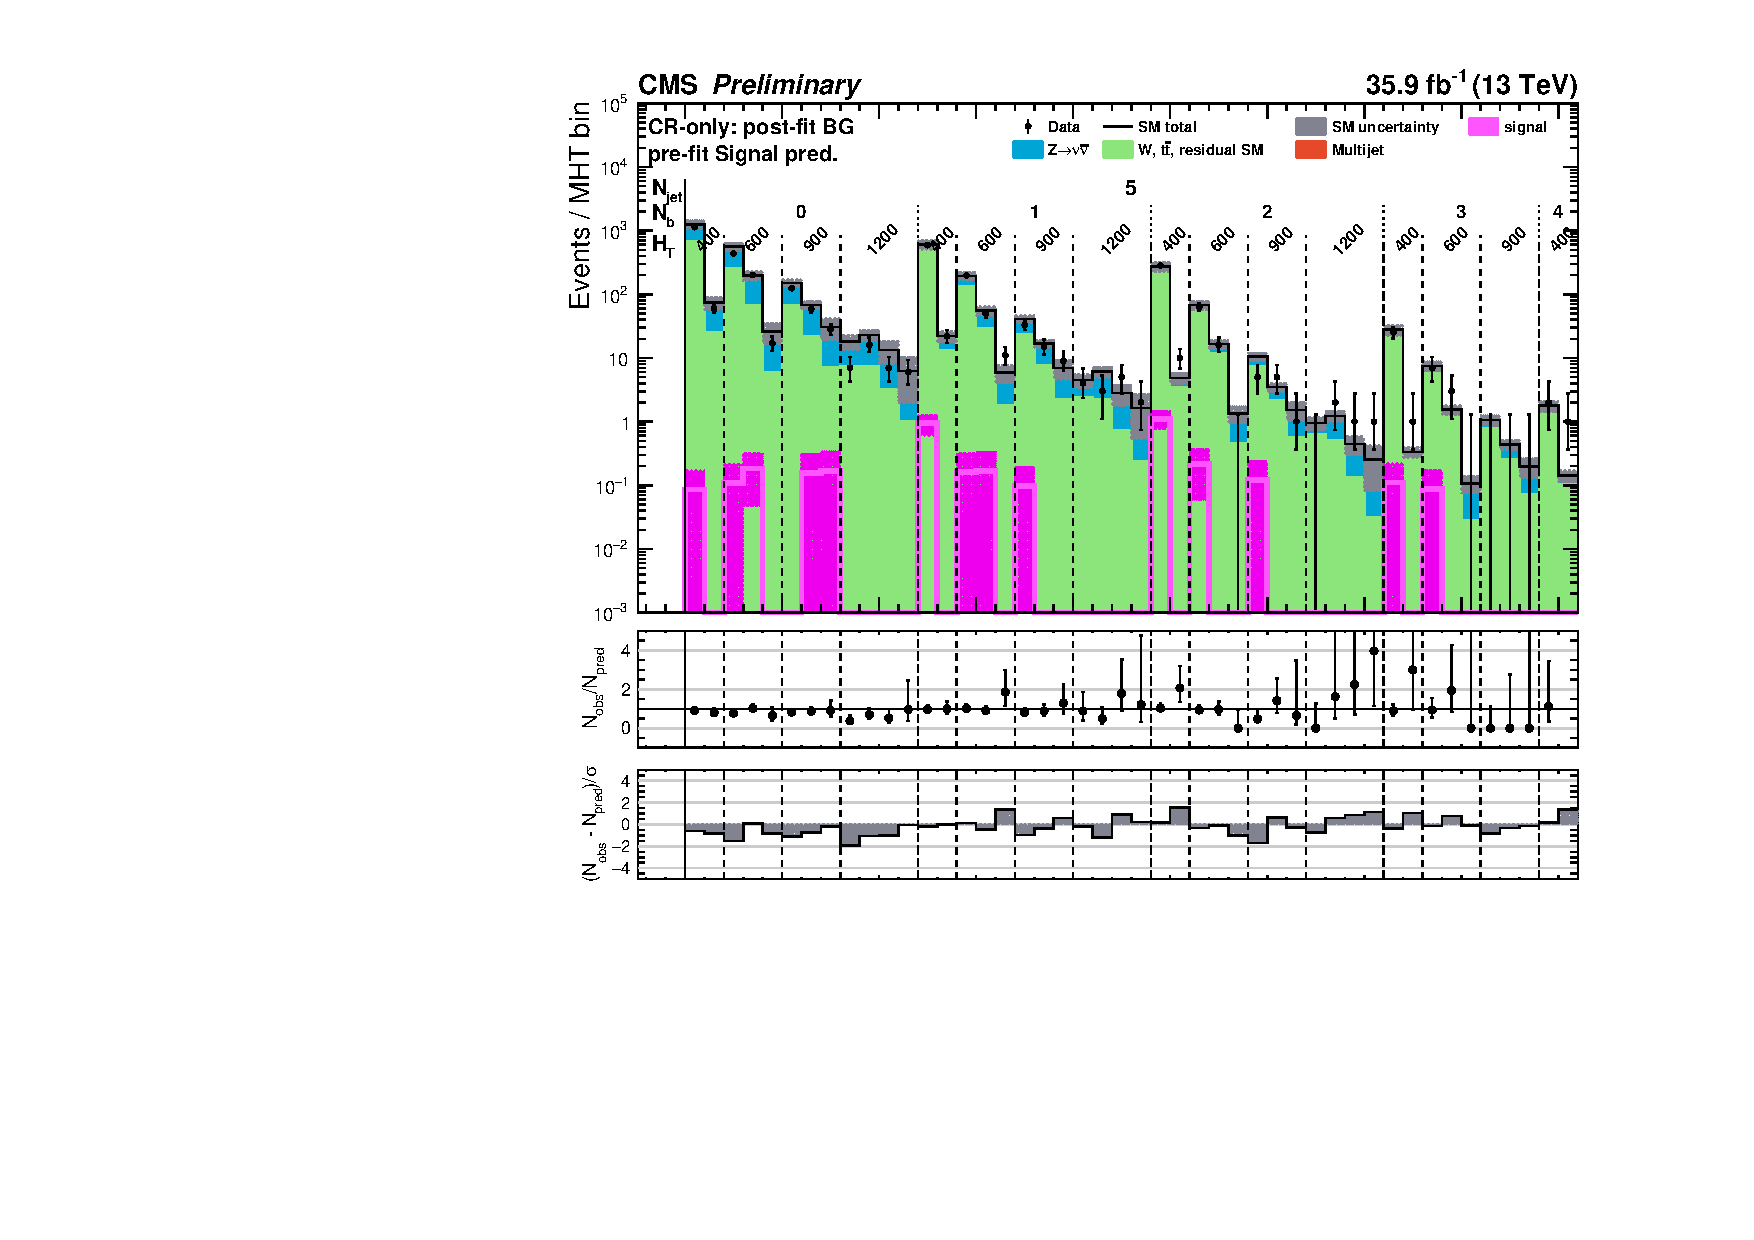
\includegraphics[width=0.49\textwidth]{figures/susyResults/app/T1tttt_mGluino-950_mLSP-600/5jet_full-fit-sig}
%        \label{fig:T1tttt_compressed_MR_5j}
%    } ~~
%    \subfigure[6+ jet]{
%        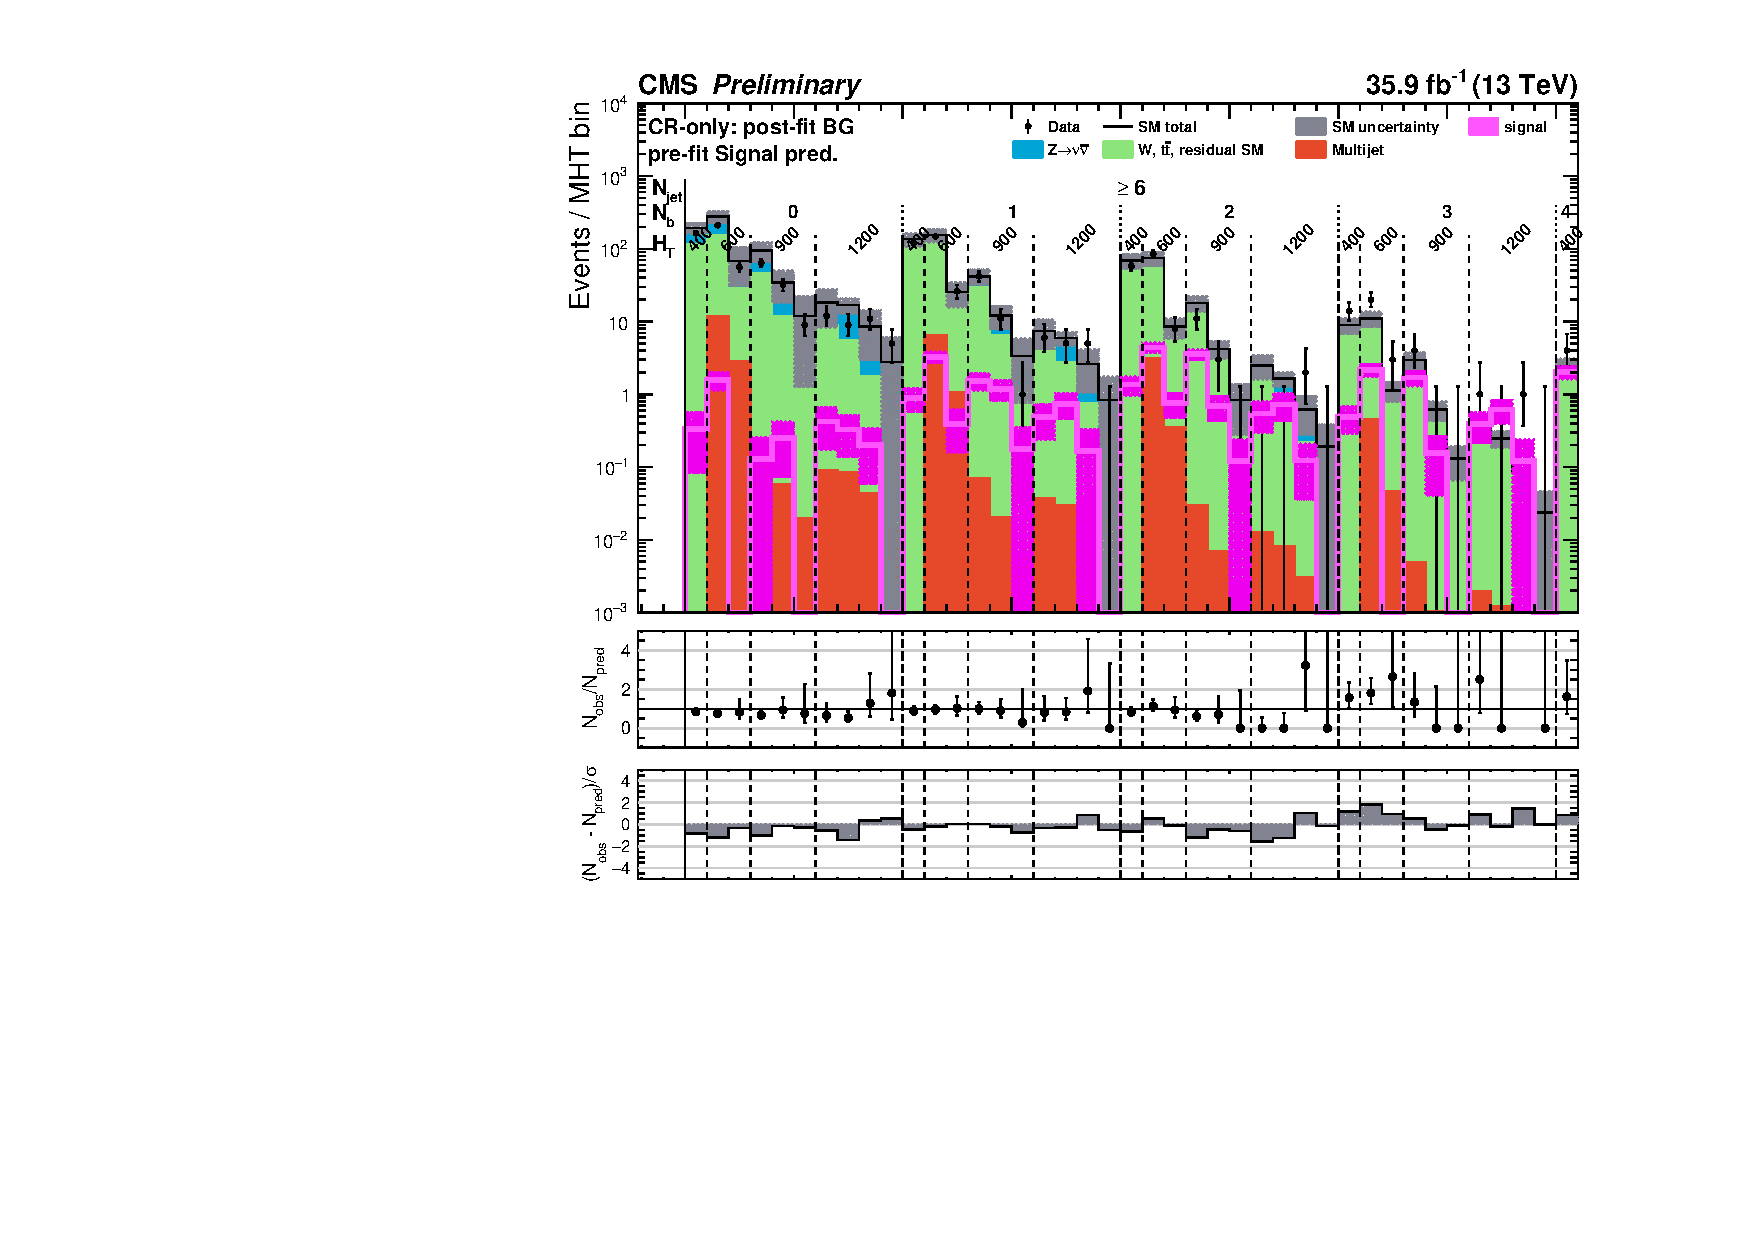
\includegraphics[width=0.49\textwidth]{figures/susyResults/app/T1tttt_mGluino-950_mLSP-600/6+_jets_full-fit-sig}
%        \label{fig:T1tttt_compressed_MR_6j}
%    } \\
%    \caption{
%        Pre-fit T1tttt compressed $(950,600)$ benchmark model overlay on
%        CR-only post-fit background prediction for all analysis bins. The
%        uncertainty on the signal model counts represents the statistical
%        uncertainty due to the finite size of the of the simulated sample.
%    }
%    \label{fig:T1tttt_compressed_MR}
%\end{figure}
%
%\begin{figure}[!h]
%    \centering
%    \subfigure[Monojet]{
%        \includegraphics[width=0.49\textwidth]{figures/susyResults/app/T1tttt_mGluino-1700_mLSP-100/monojet_full-fit-sig}
%        \label{fig:T1tttt_uncompressed_MR_1j}
%    } ~~
%    \subfigure[Di-jet]{
%        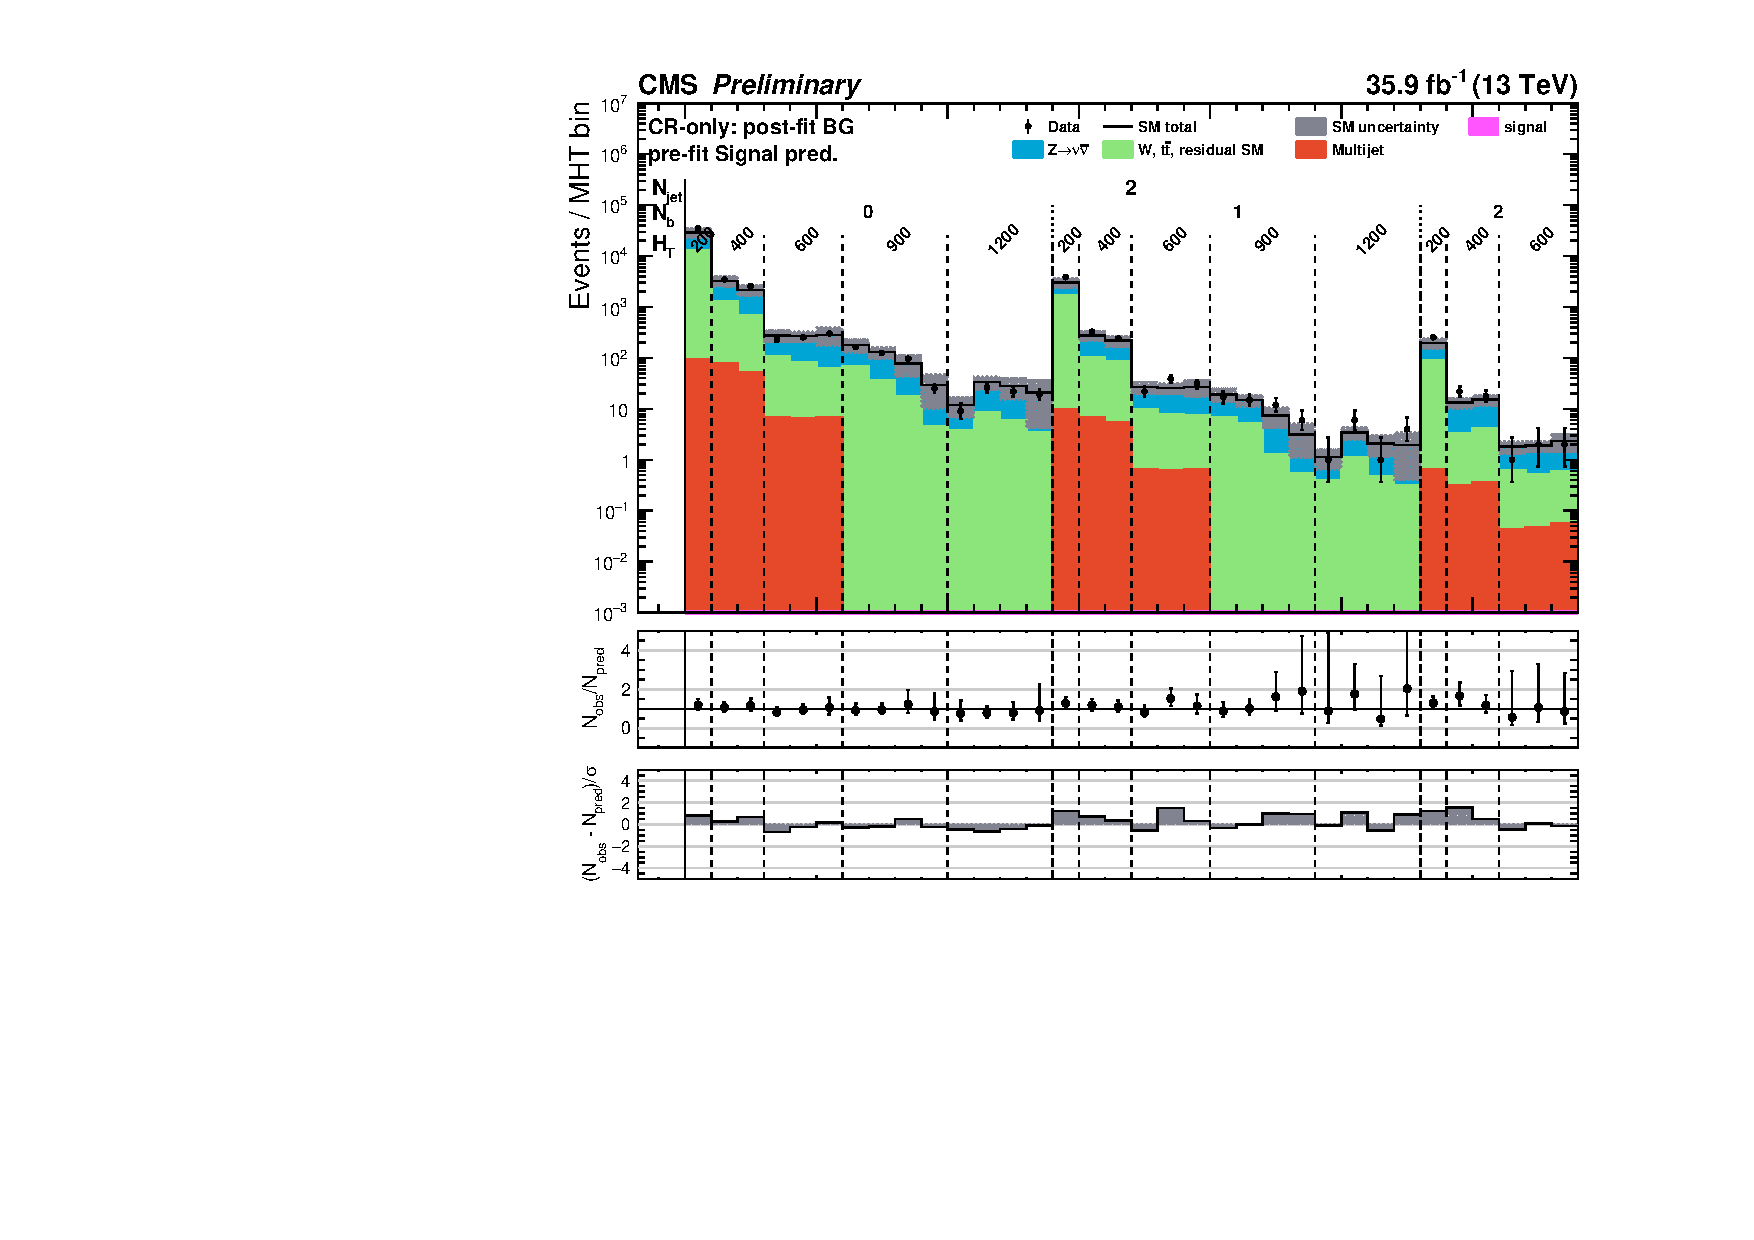
\includegraphics[width=0.49\textwidth]{figures/susyResults/app/T1tttt_mGluino-1700_mLSP-100/di-jet_full-fit-sig}
%        \label{fig:T1tttt_uncompressed_MR_2j}
%    } \\
%    \subfigure[3 jet]{
%        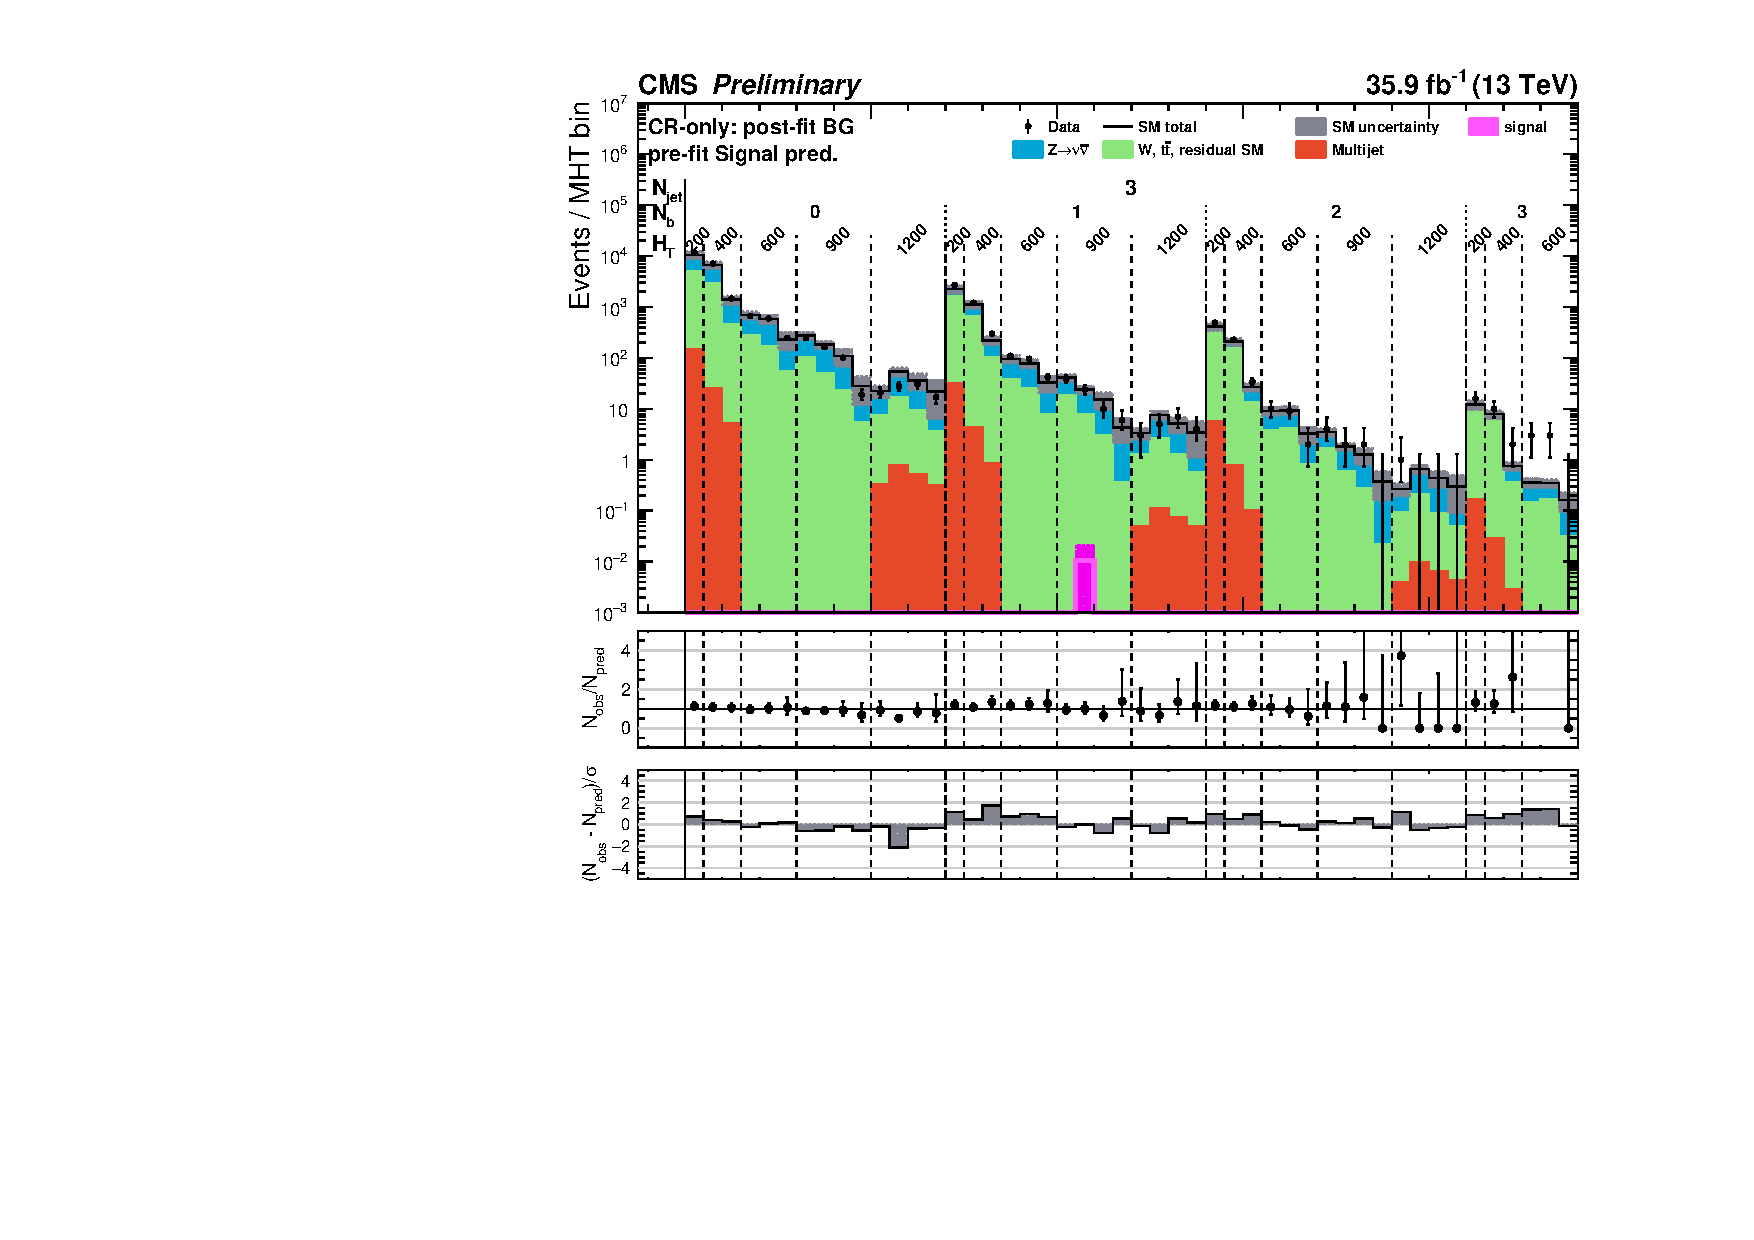
\includegraphics[width=0.49\textwidth]{figures/susyResults/app/T1tttt_mGluino-1700_mLSP-100/3jet_full-fit-sig}
%        \label{fig:T1tttt_uncompressed_MR_3j}
%    } ~~
%    \subfigure[4 jet]{
%        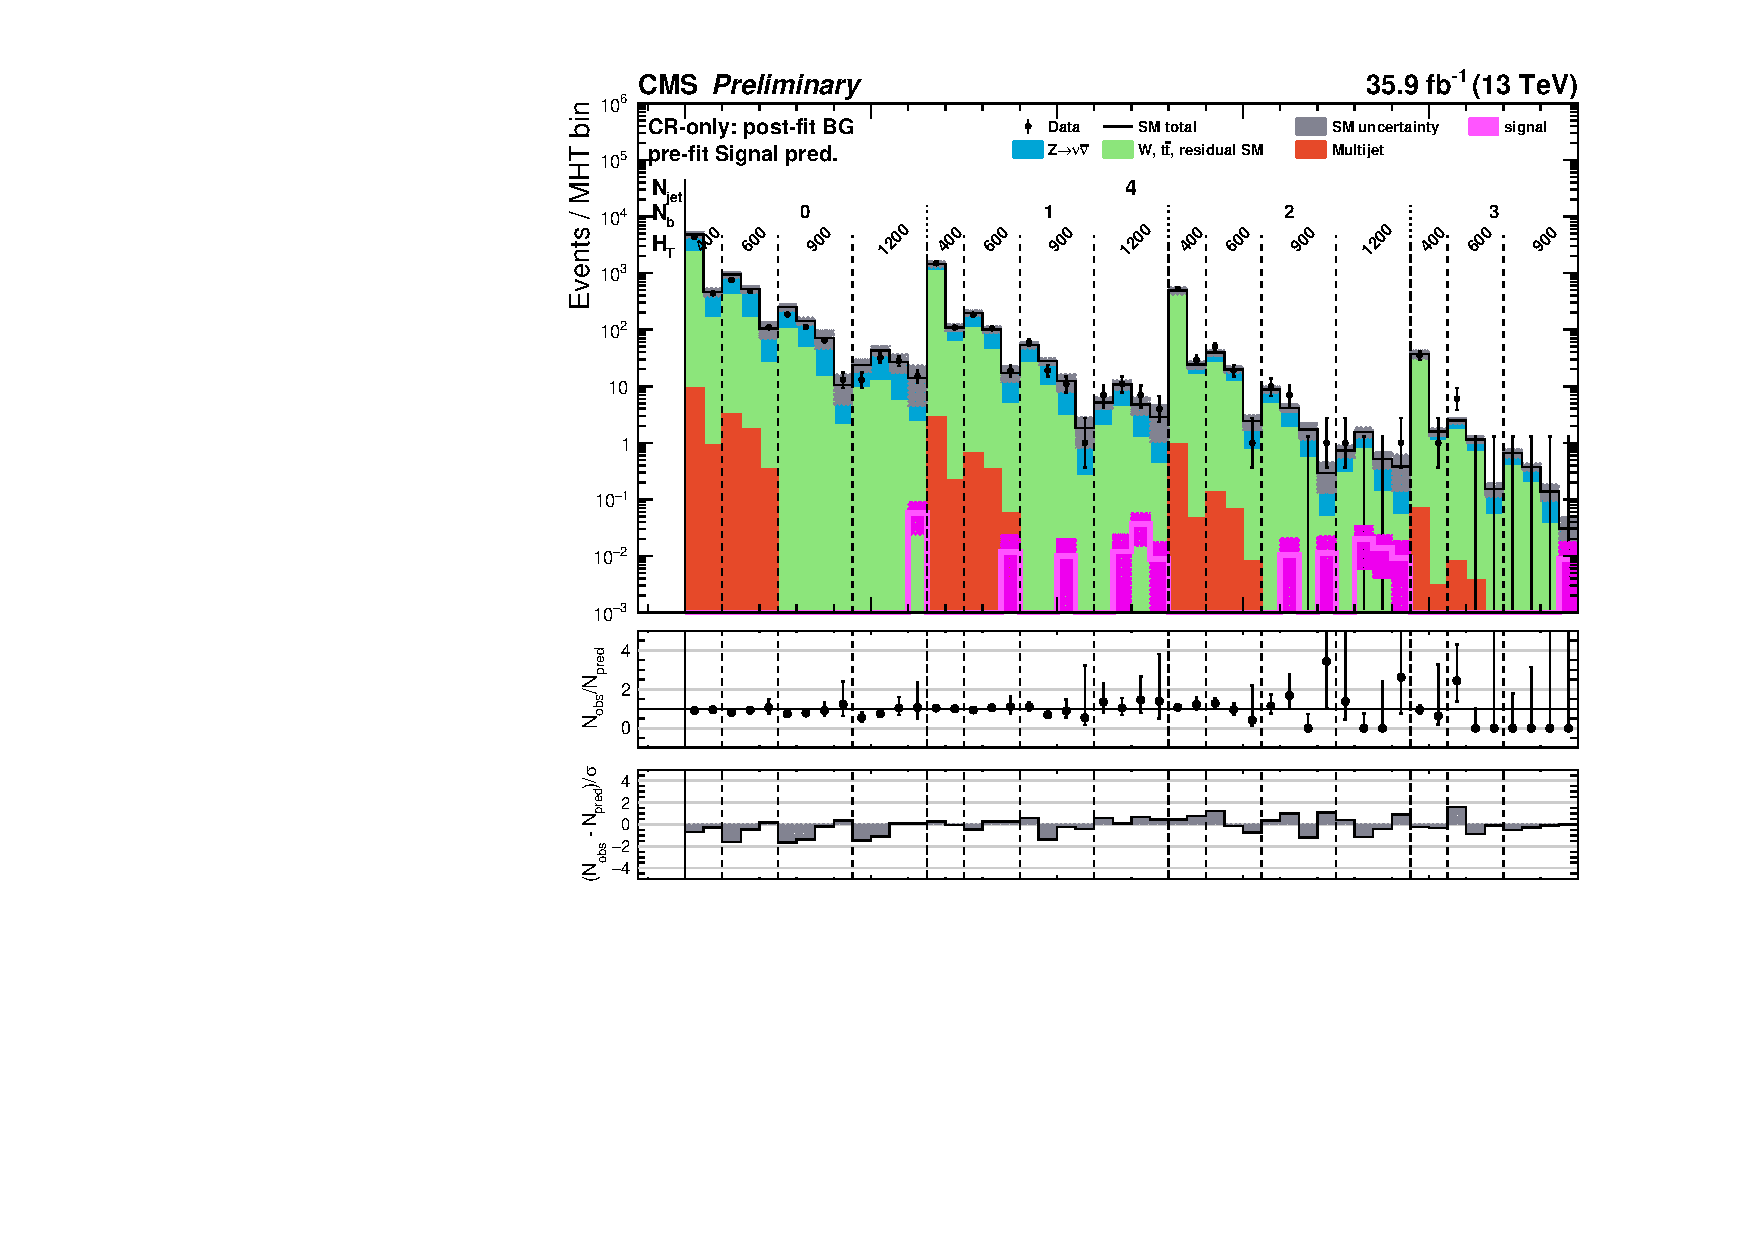
\includegraphics[width=0.49\textwidth]{figures/susyResults/app/T1tttt_mGluino-1700_mLSP-100/4jet_full-fit-sig}
%        \label{fig:T1tttt_uncompressed_MR_4j}
%    } \\
%    \subfigure[5 jet]{
%        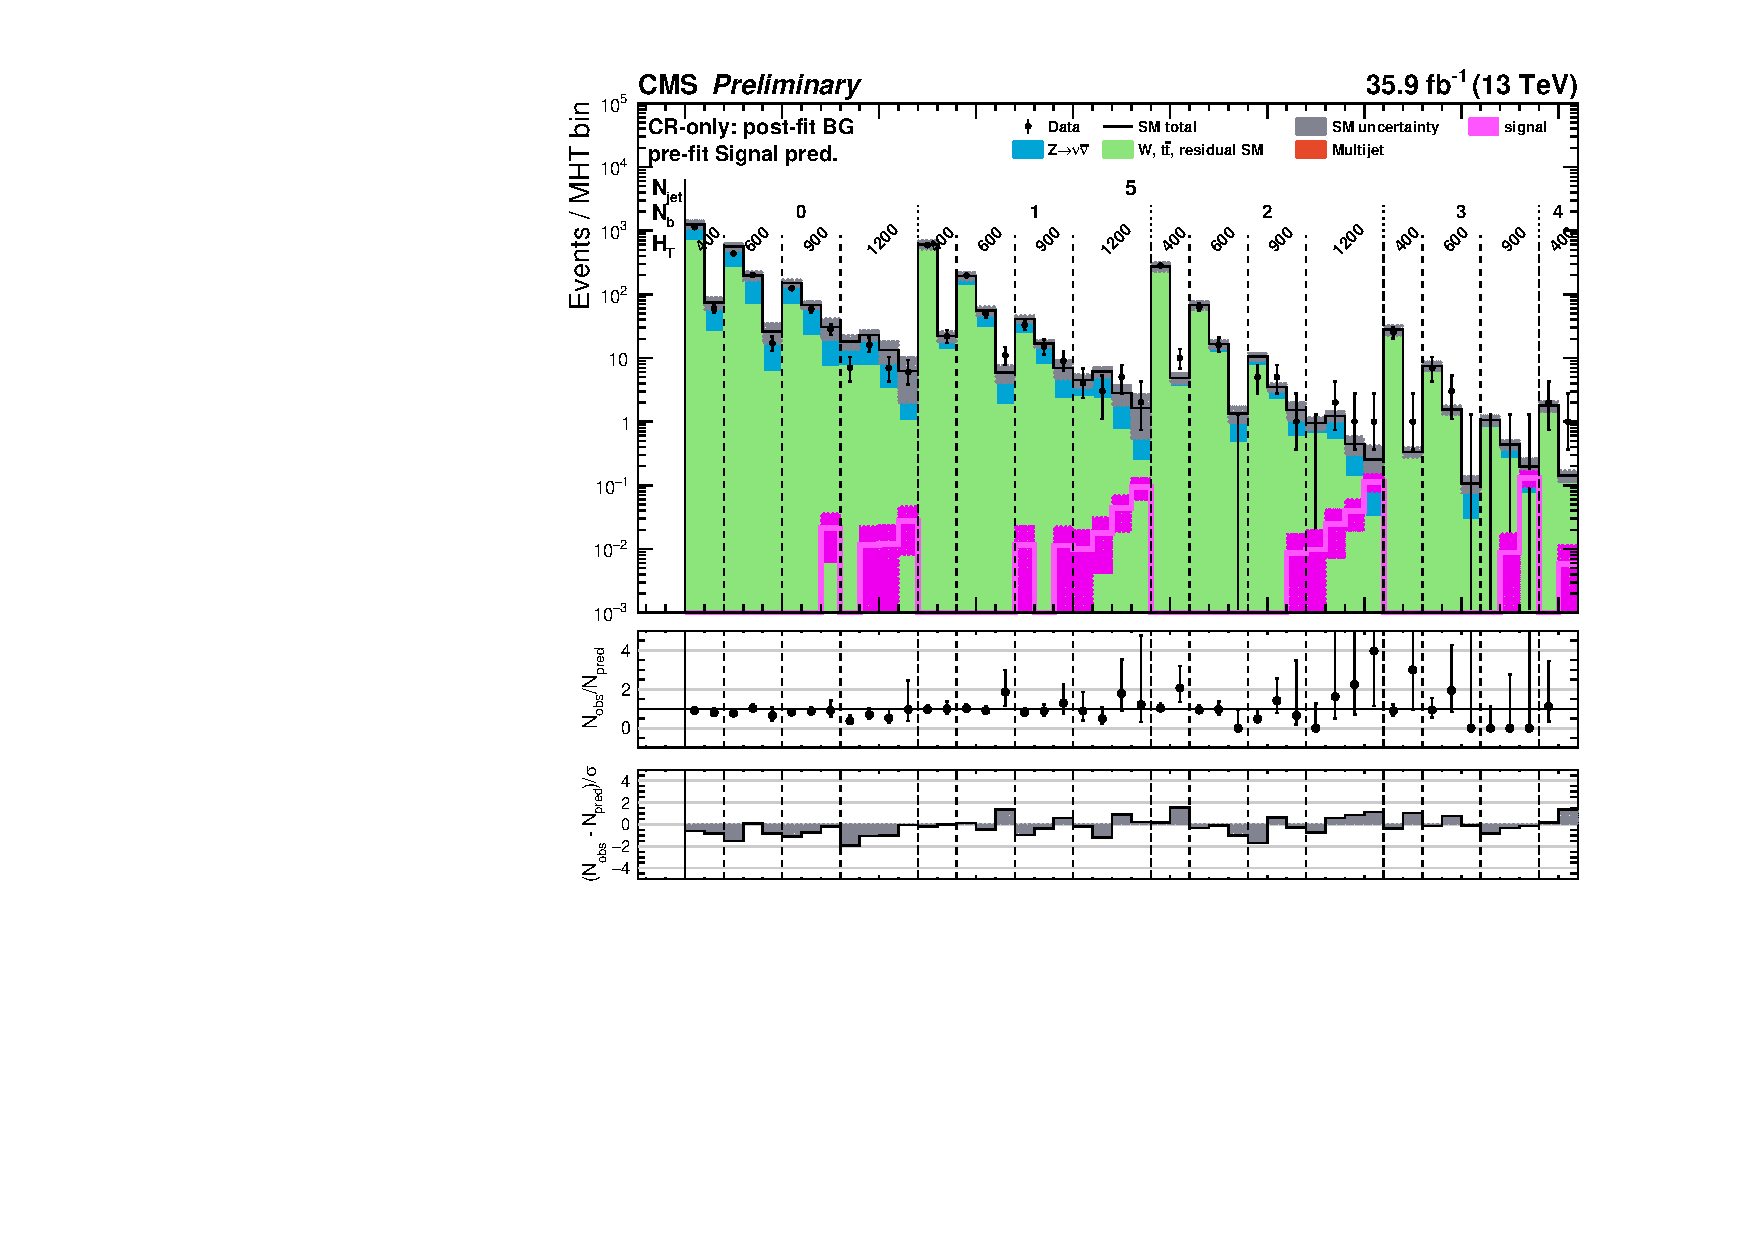
\includegraphics[width=0.49\textwidth]{figures/susyResults/app/T1tttt_mGluino-1700_mLSP-100/5jet_full-fit-sig}
%        \label{fig:T1tttt_uncompressed_MR_5j}
%    } ~~
%    \subfigure[6+ jet]{
%        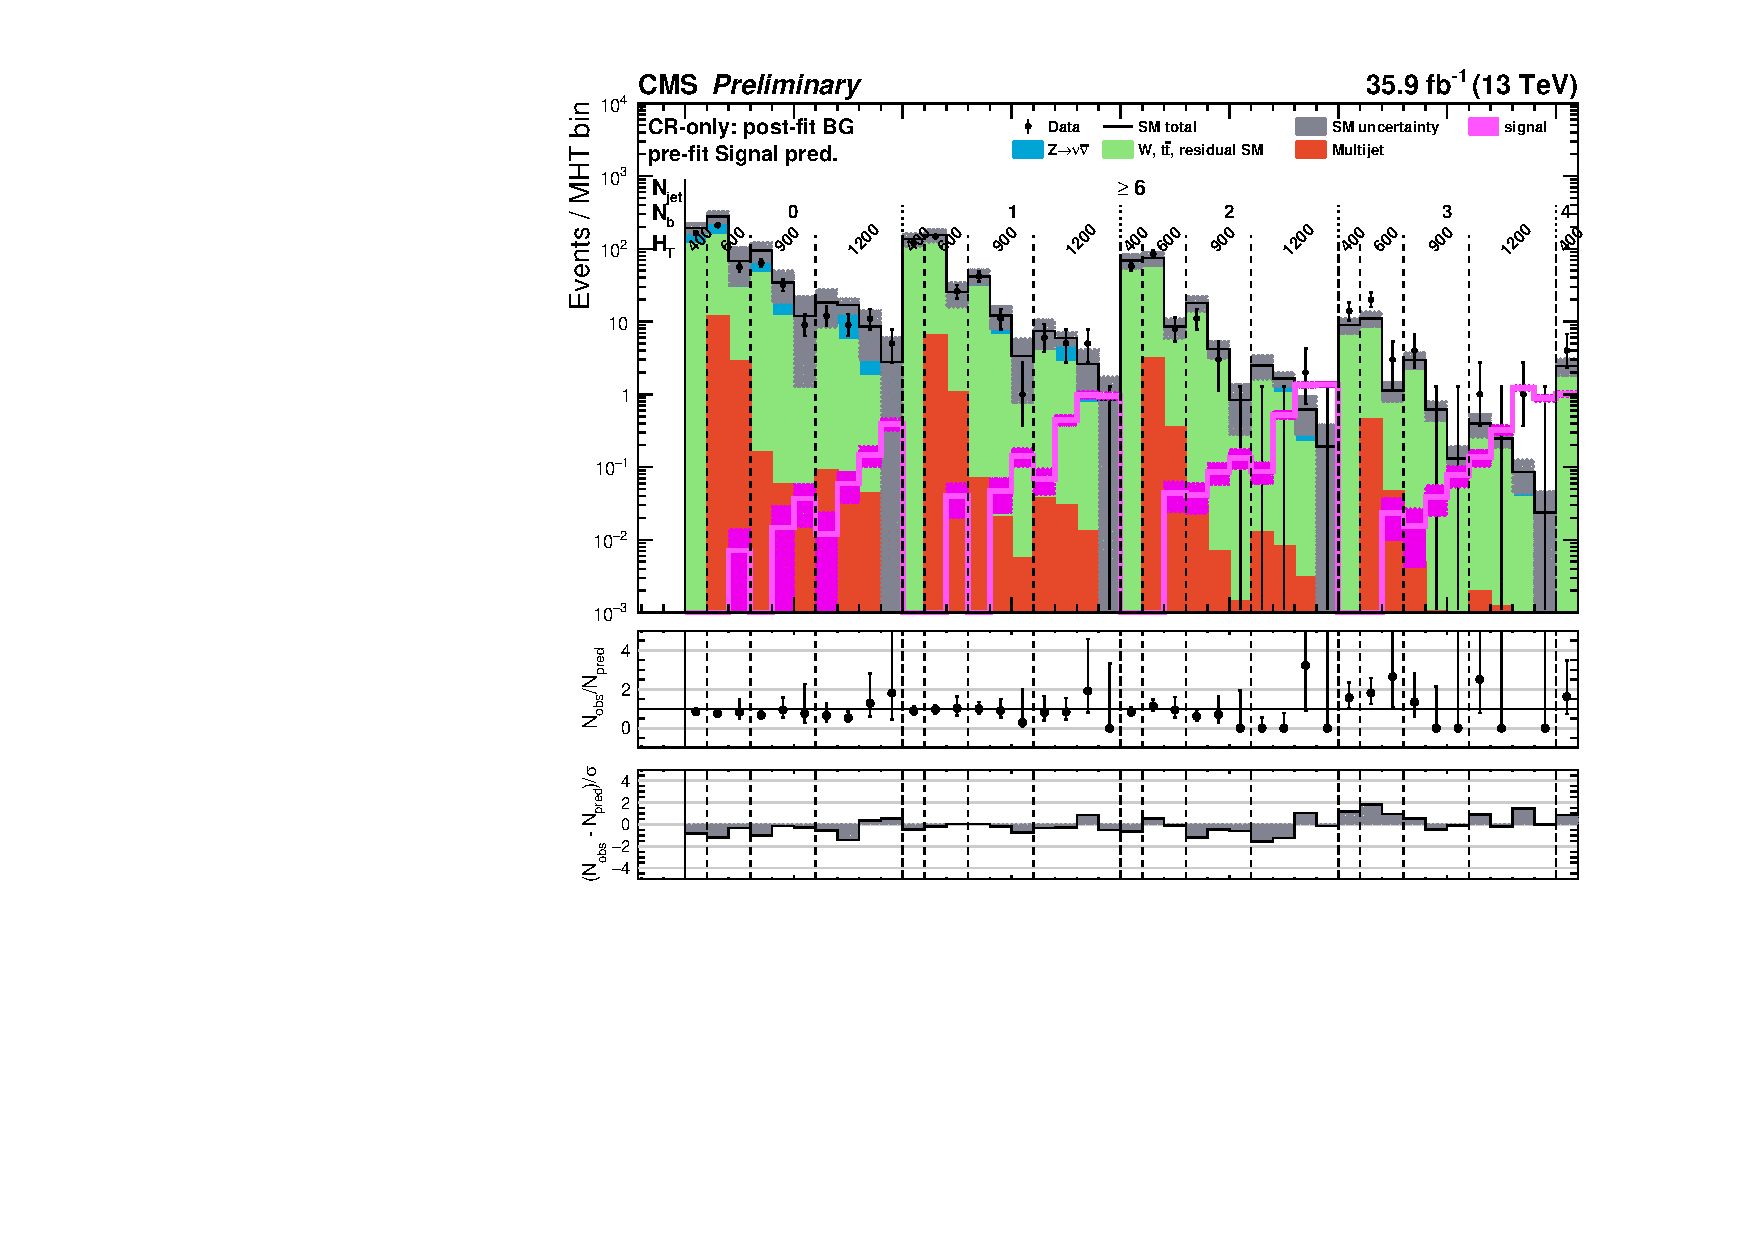
\includegraphics[width=0.49\textwidth]{figures/susyResults/app/T1tttt_mGluino-1700_mLSP-100/6+_jets_full-fit-sig}
%        \label{fig:T1tttt_uncompressed_MR_6j}
%    } \\
%    \caption{
%        Pre-fit T1tttt uncompressed $(1700,100)$ benchmark model overlay on
%        CR-only post-fit background prediction for all analysis bins. The
%        uncertainty on the signal model counts represents the statistical
%        uncertainty due to the finite size of the of the simulated sample.
%    }
%    \label{fig:T1tttt_uncompressed_MR}
%\end{figure}
%
%\begin{figure}[!h]
%    \centering
%    \subfigure[Monojet]{
%        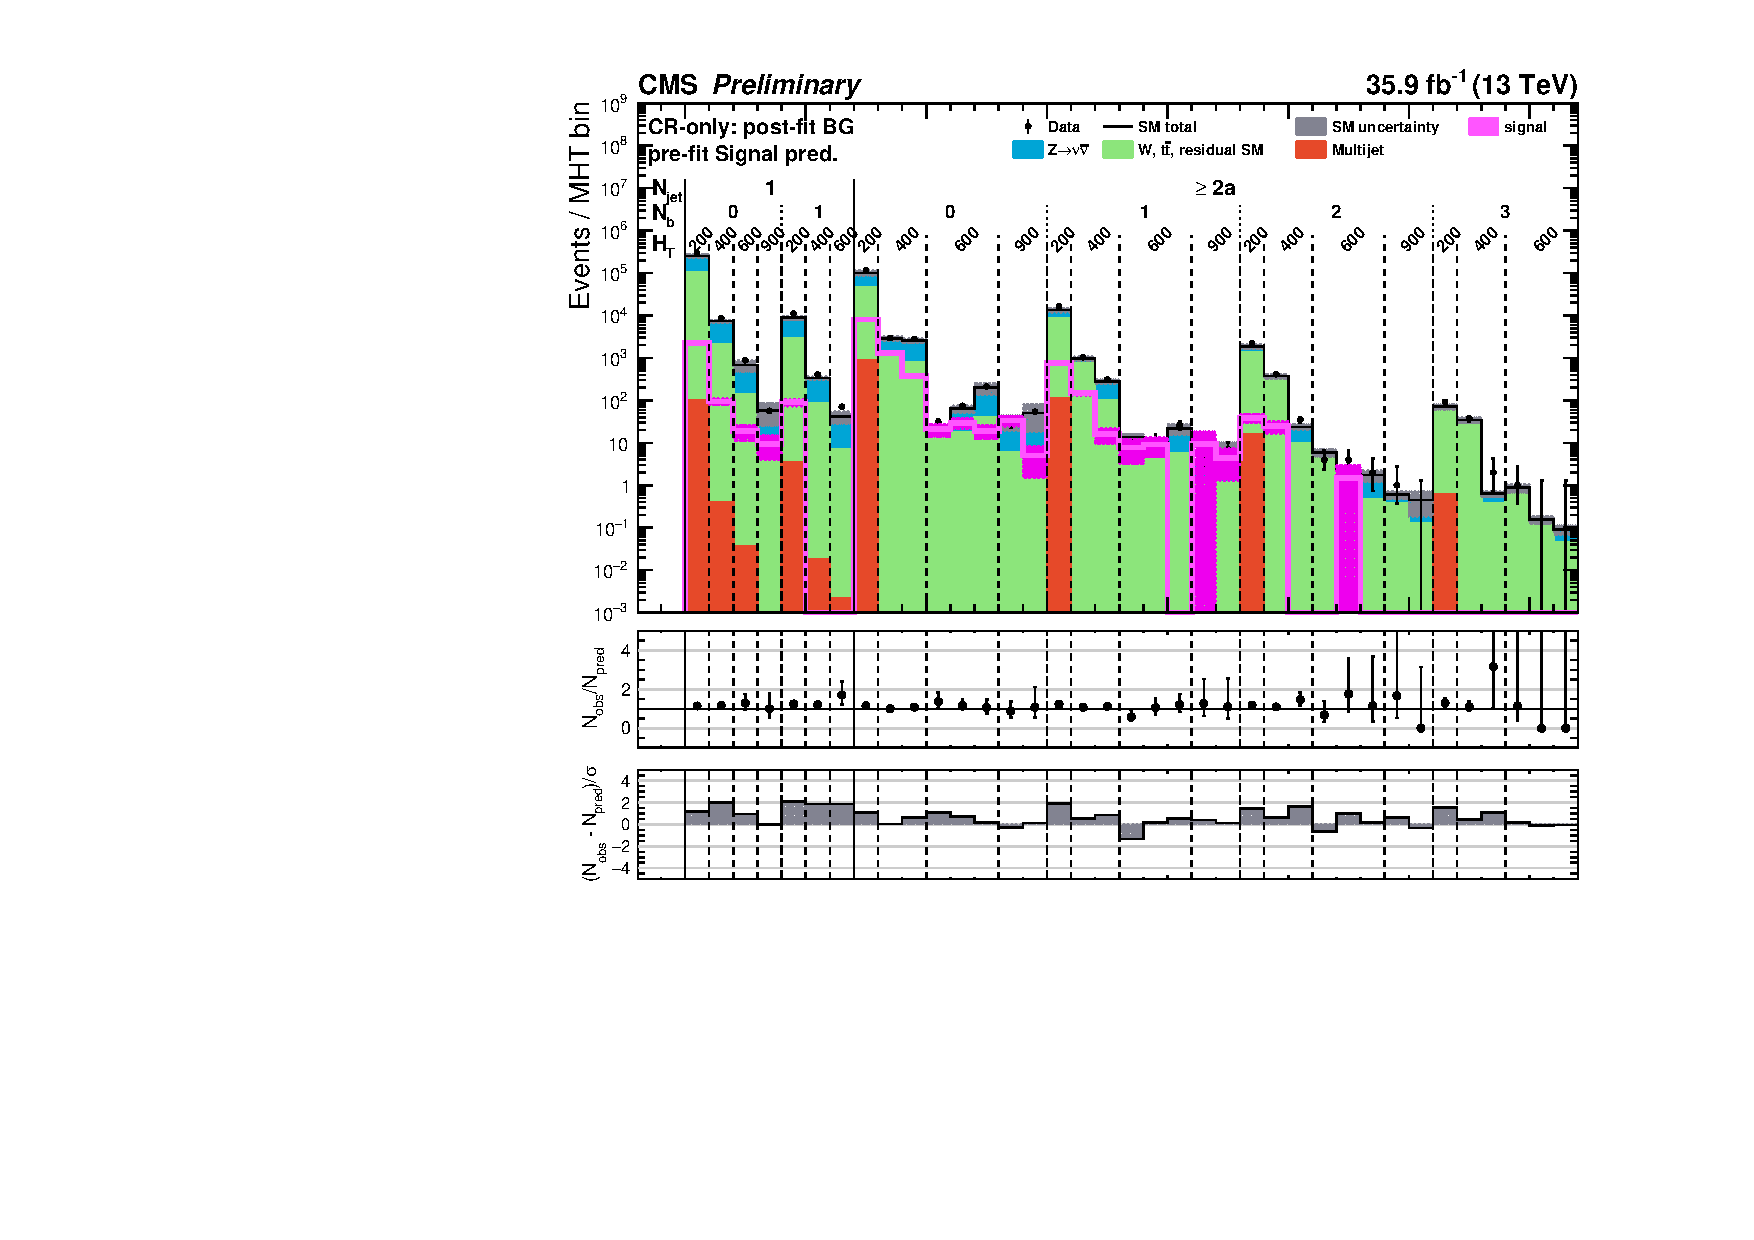
\includegraphics[width=0.49\textwidth]{figures/susyResults/app/T2qq_mSquark-400_mLSP-300/monojet_full-fit-sig}
%        \label{fig:T2qq_1fold_compressed_MR_1j}
%    } ~~
%    \subfigure[Di-jet]{
%        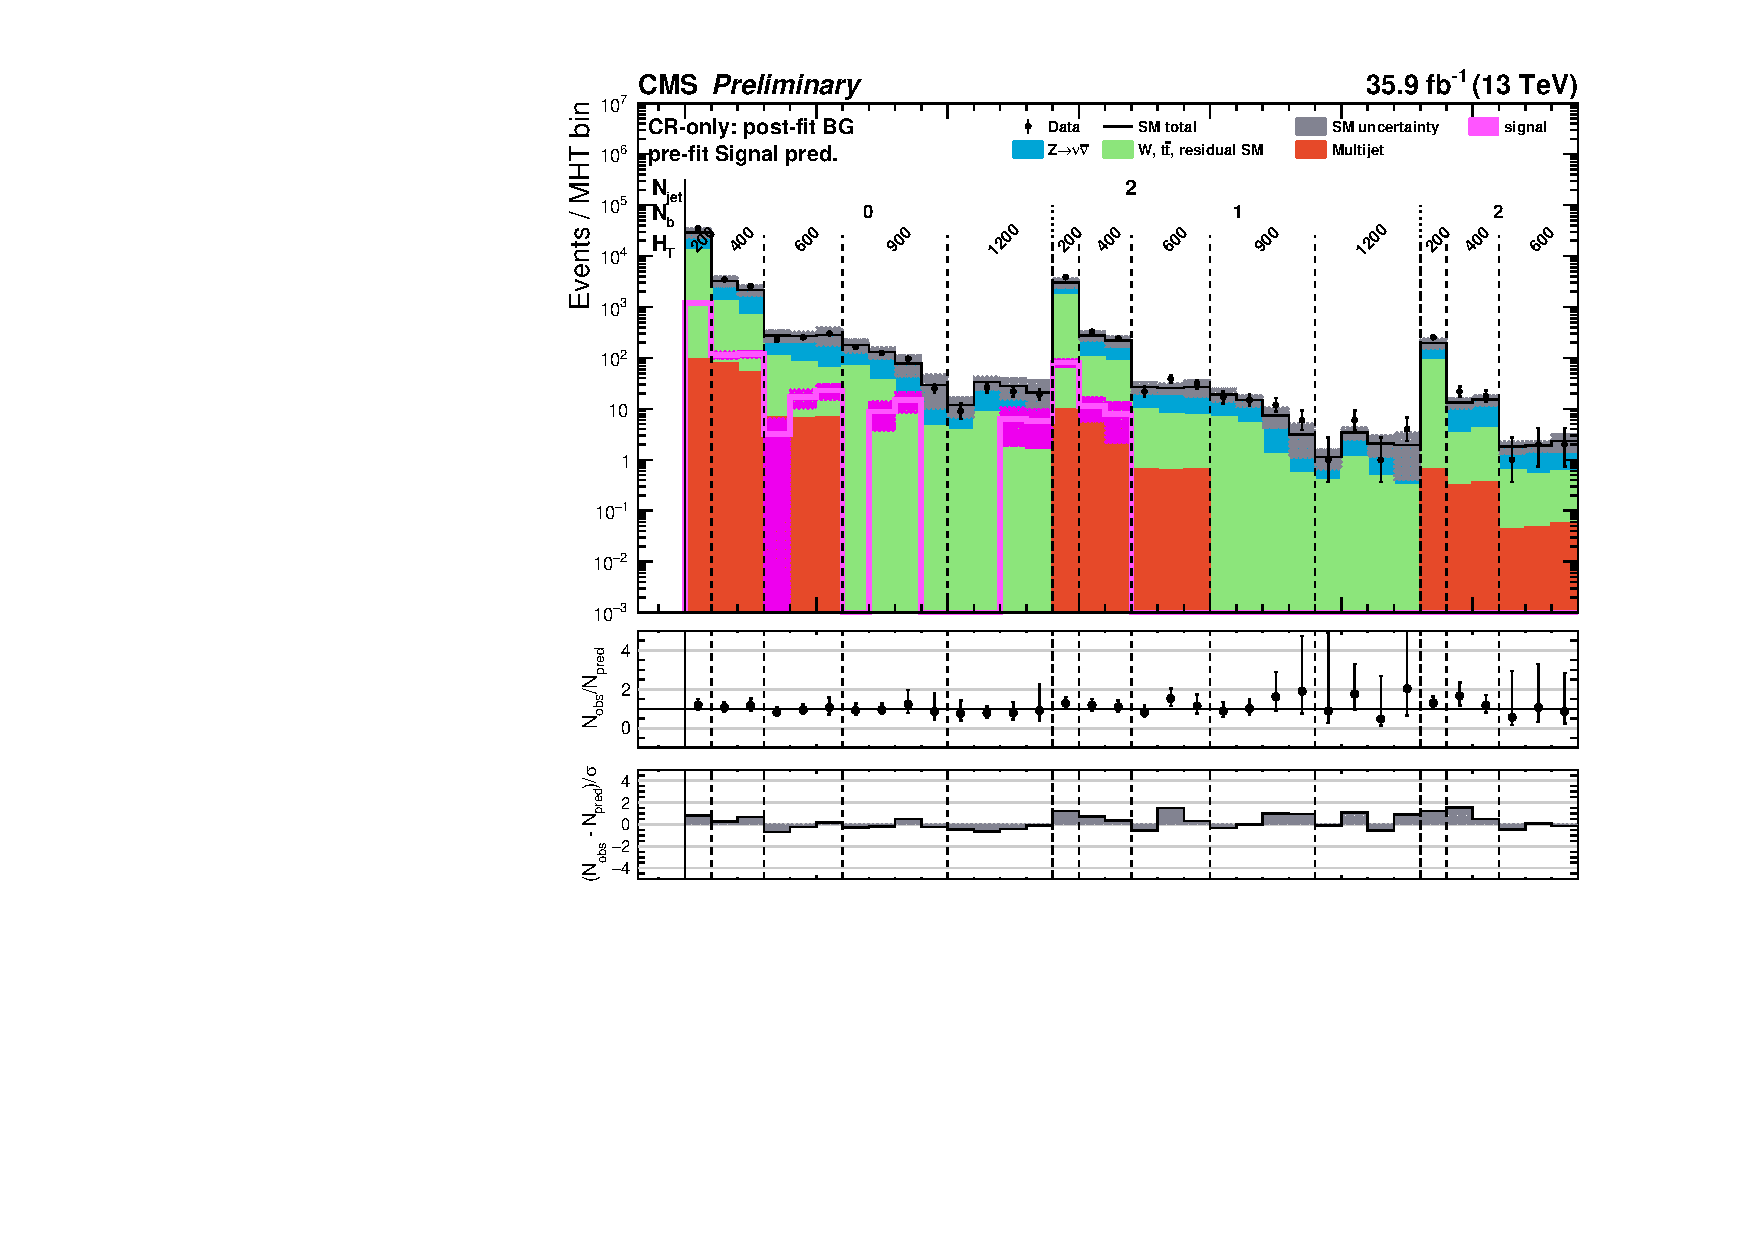
\includegraphics[width=0.49\textwidth]{figures/susyResults/app/T2qq_mSquark-400_mLSP-300/di-jet_full-fit-sig}
%        \label{fig:T2qq_1fold_compressed_MR_2j}
%    } \\
%    \subfigure[3 jet]{
%        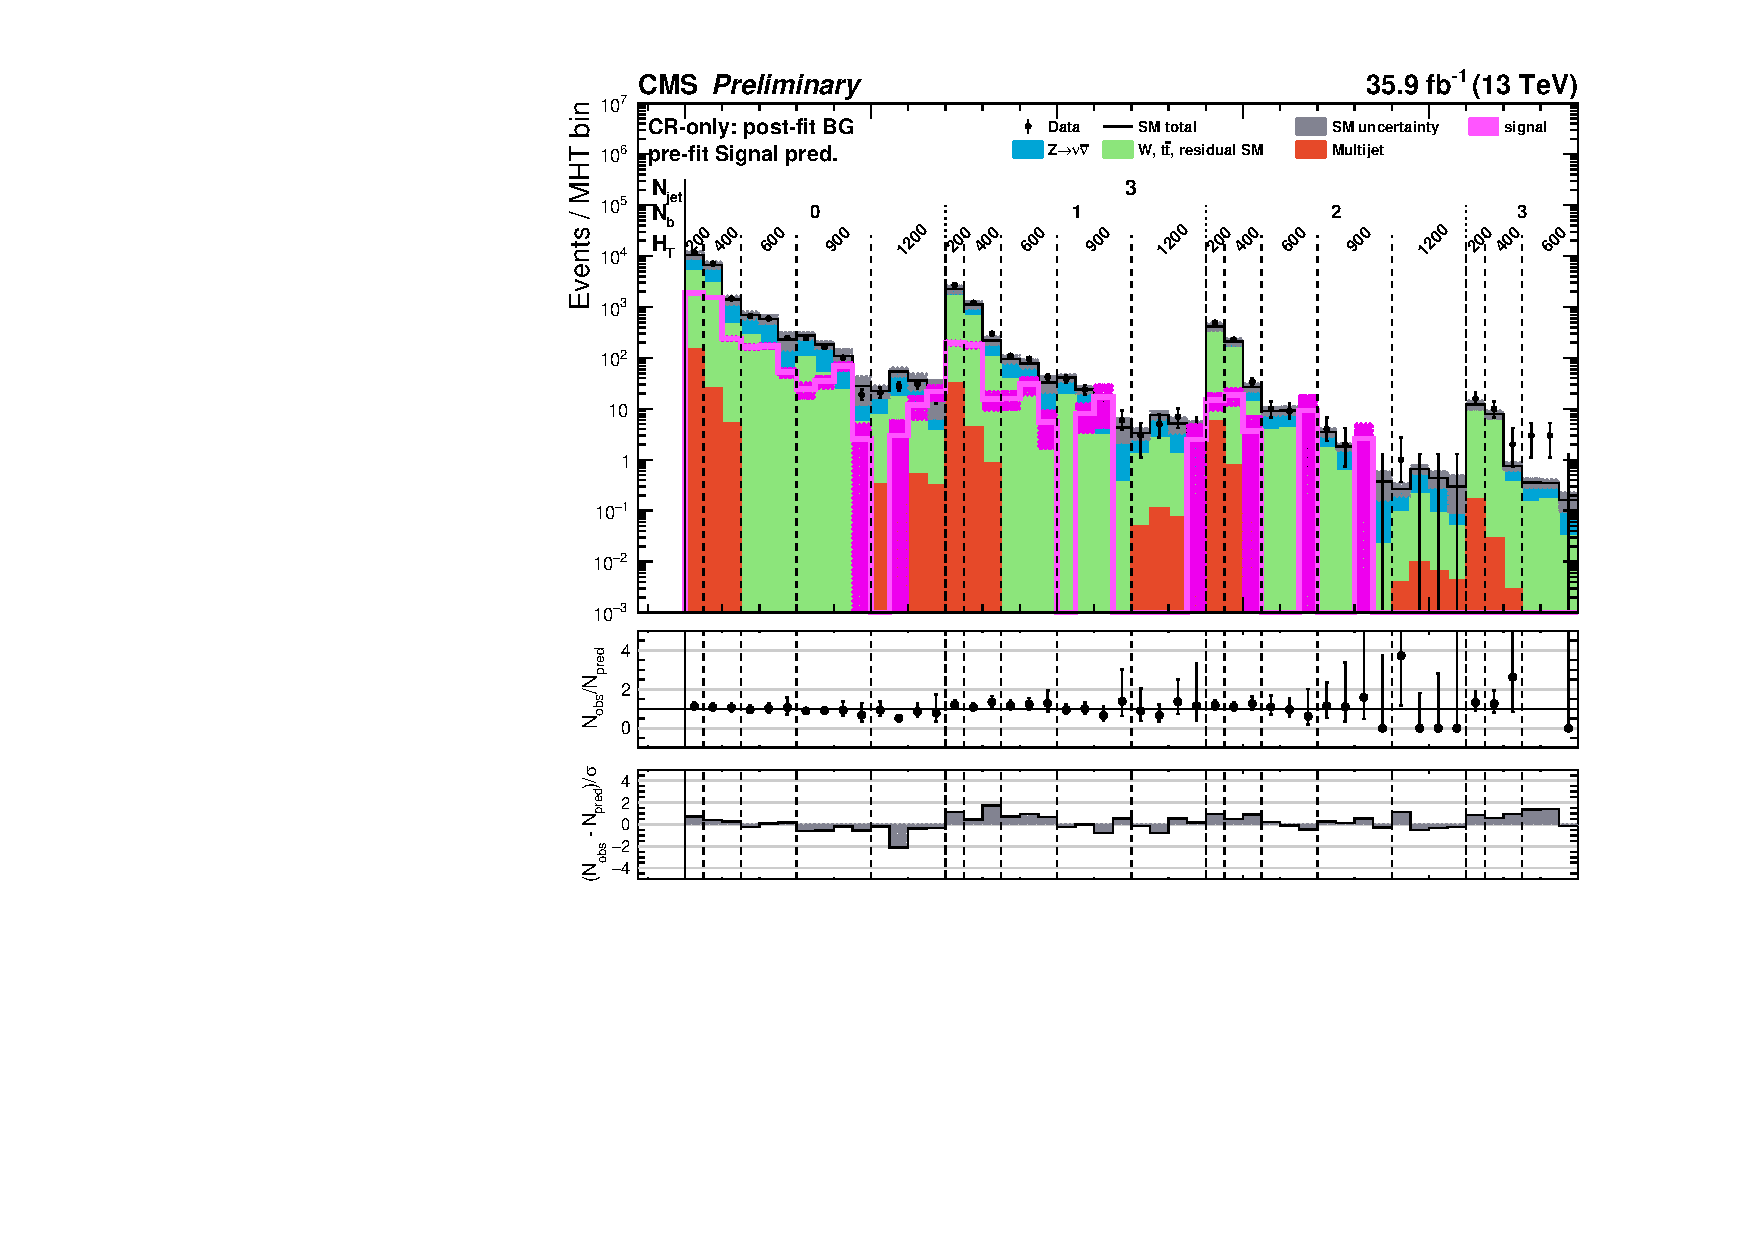
\includegraphics[width=0.49\textwidth]{figures/susyResults/app/T2qq_mSquark-400_mLSP-300/3jet_full-fit-sig}
%        \label{fig:T2qq_1fold_compressed_MR_3j}
%    } ~~
%    \subfigure[4 jet]{
%        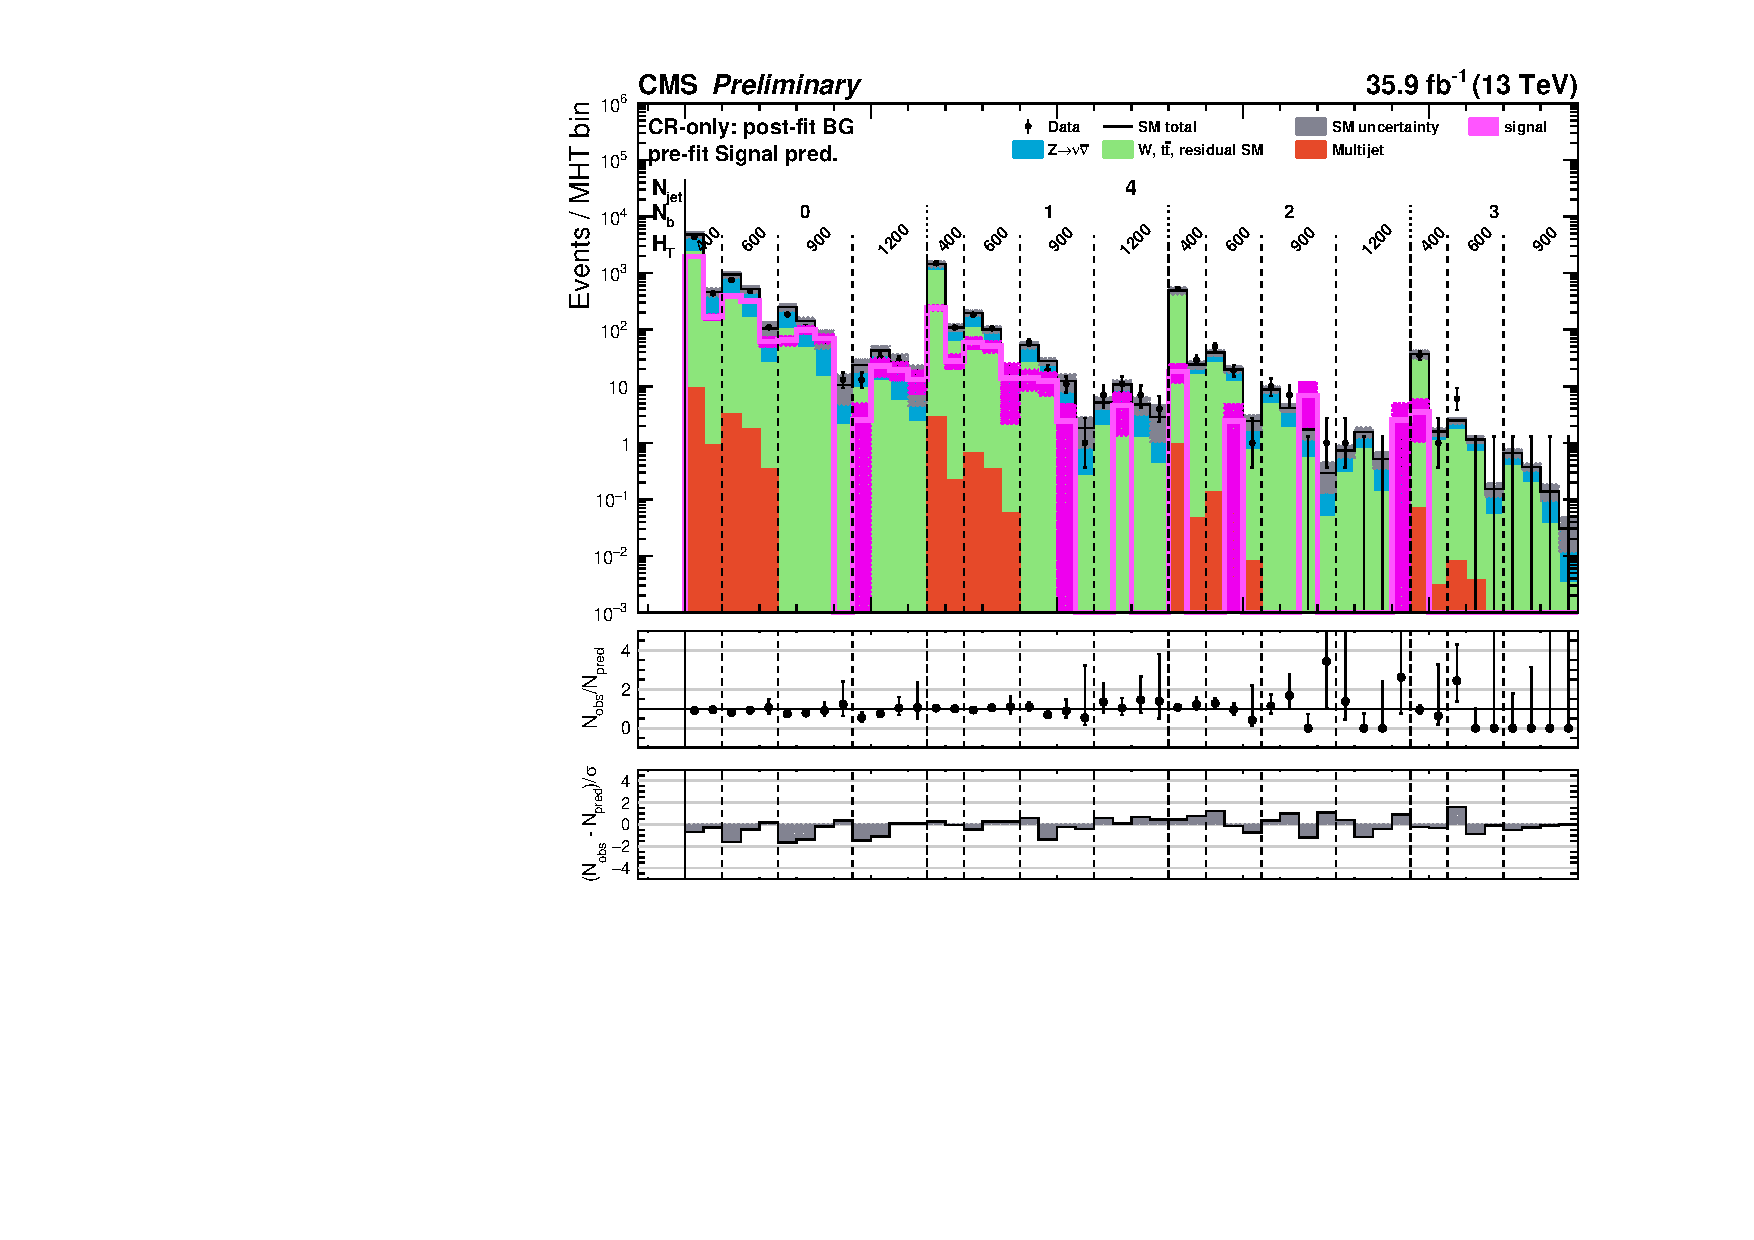
\includegraphics[width=0.49\textwidth]{figures/susyResults/app/T2qq_mSquark-400_mLSP-300/4jet_full-fit-sig}
%        \label{fig:T2qq_1fold_compressed_MR_4j}
%    } \\
%    \subfigure[5 jet]{
%        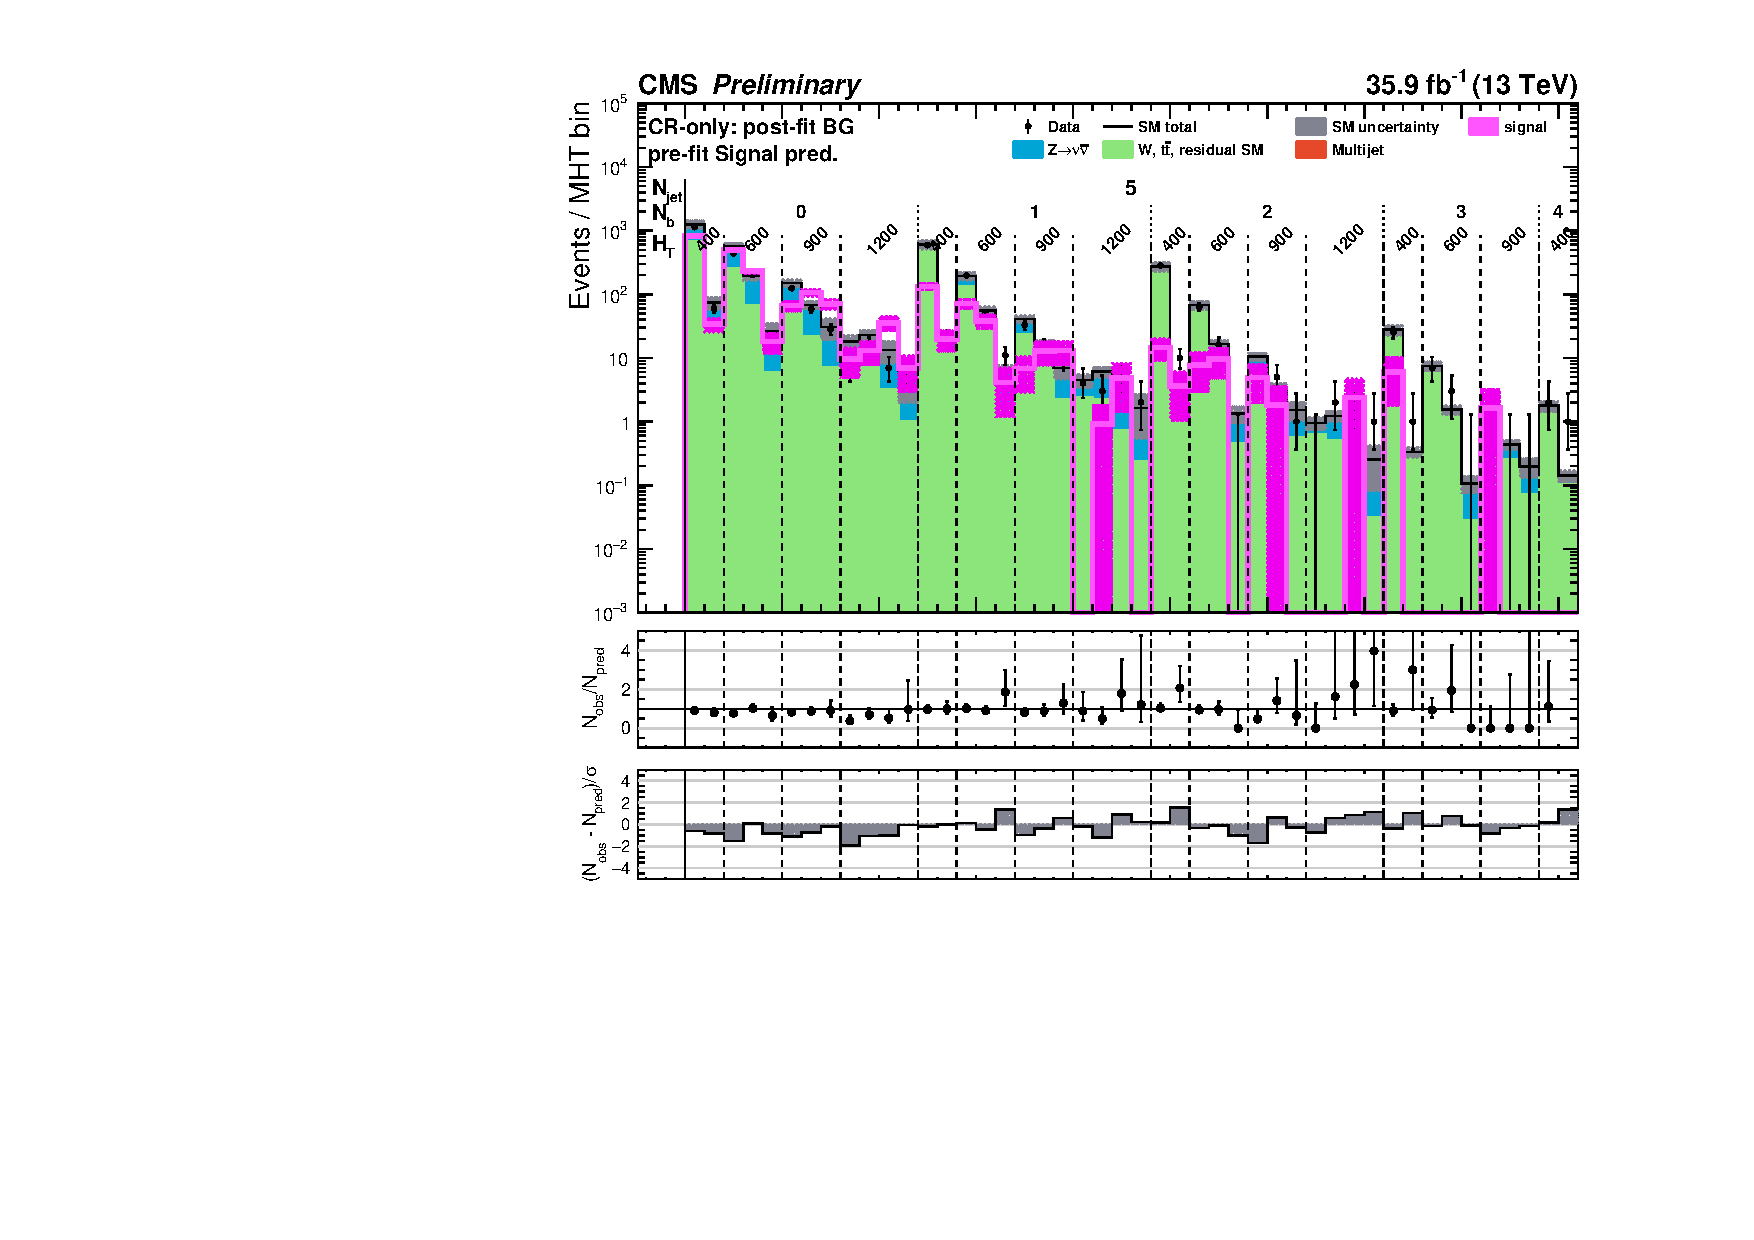
\includegraphics[width=0.49\textwidth]{figures/susyResults/app/T2qq_mSquark-400_mLSP-300/5jet_full-fit-sig}
%        \label{fig:T2qq_1fold_compressed_MR_5j}
%    } ~~
%    \subfigure[6+ jet]{
%        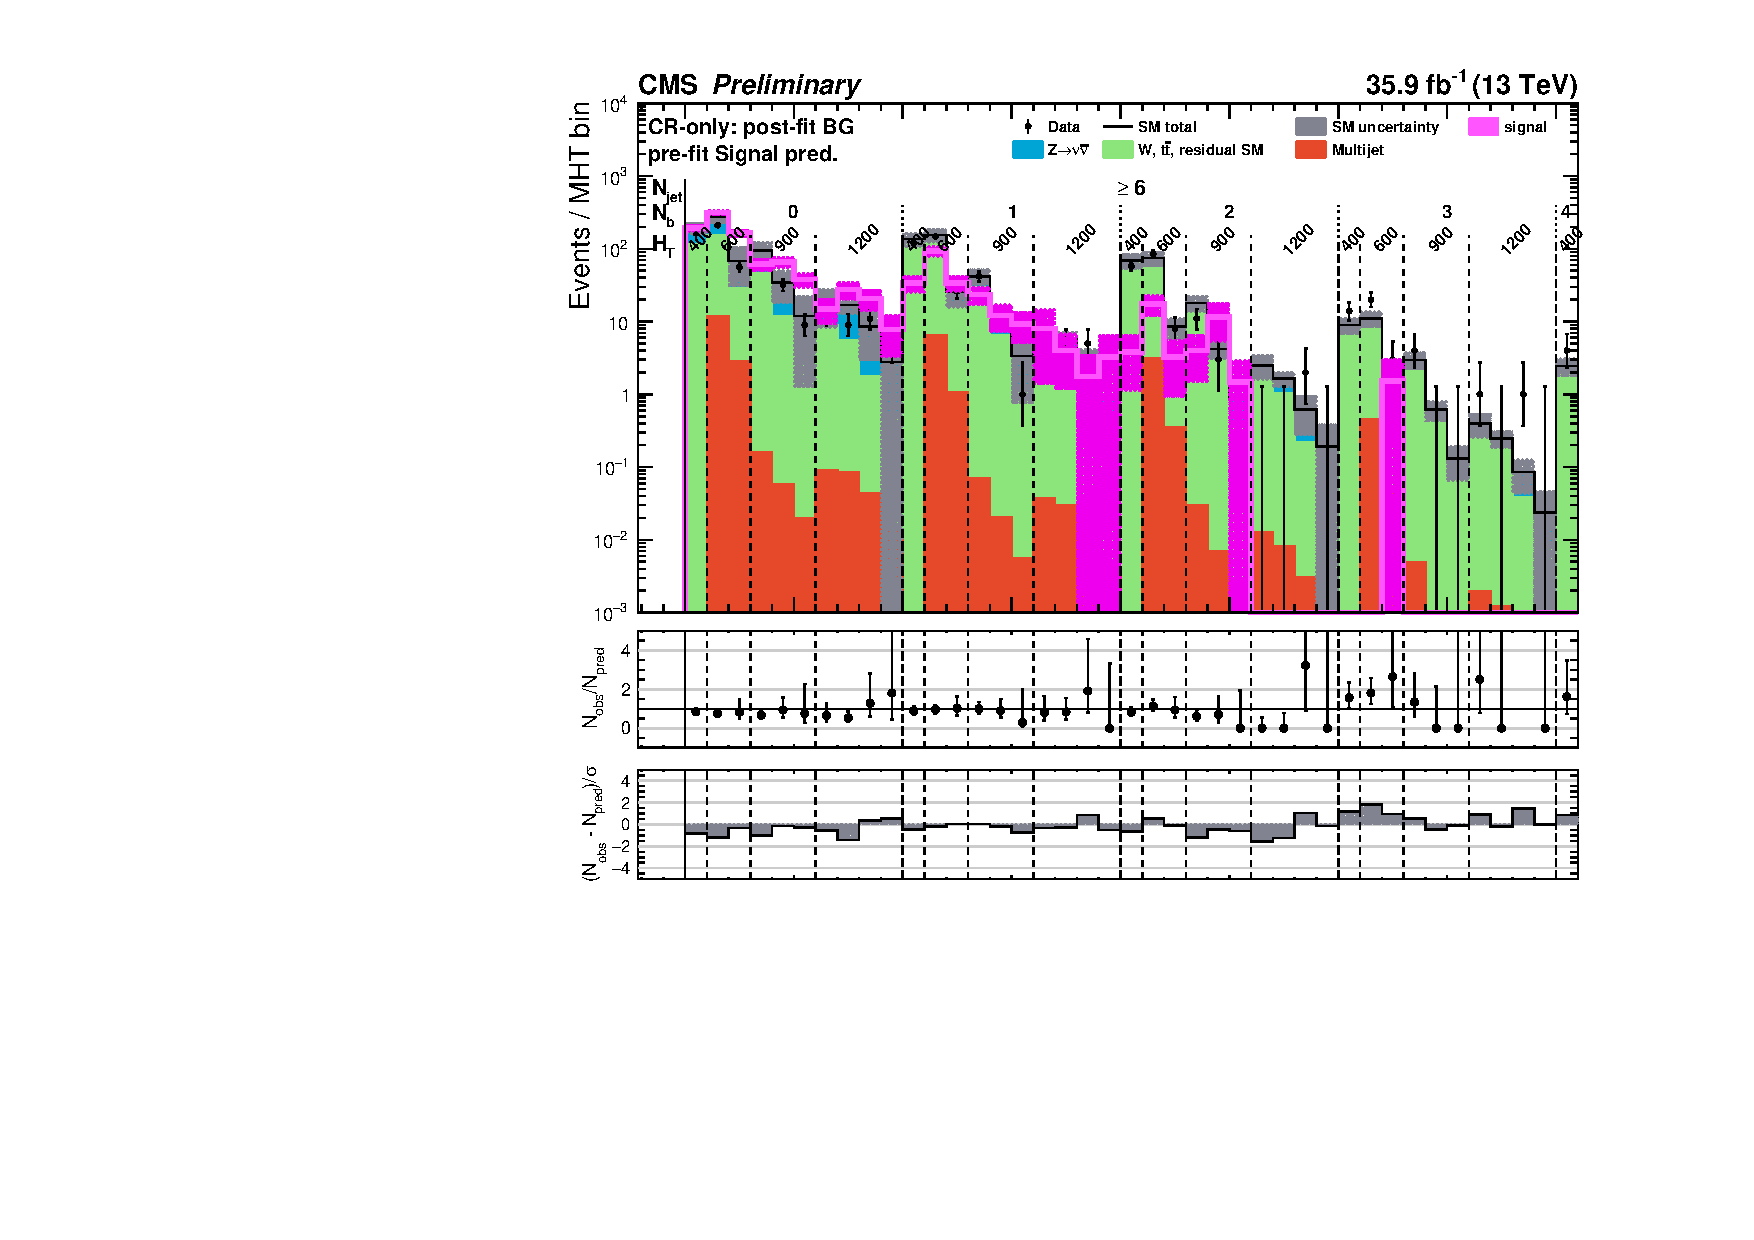
\includegraphics[width=0.49\textwidth]{figures/susyResults/app/T2qq_mSquark-400_mLSP-300/6+_jets_full-fit-sig}
%        \label{fig:T2qq_1fold_compressed_MR_6j}
%    } \\
%    \caption{
%        Pre-fit T2qq compressed $(400,300)$ benchmark model overlay on CR-only
%        post-fit background prediction for all analysis bins. The uncertainty
%        on the signal model counts represents the statistical uncertainty due
%        to the finite size of the of the simulated sample.
%    }
%    \label{fig:T2qq_1fold_compressed_MR}
%\end{figure}
%
%\begin{figure}[!h]
%    \centering
%    \subfigure[Monojet]{
%        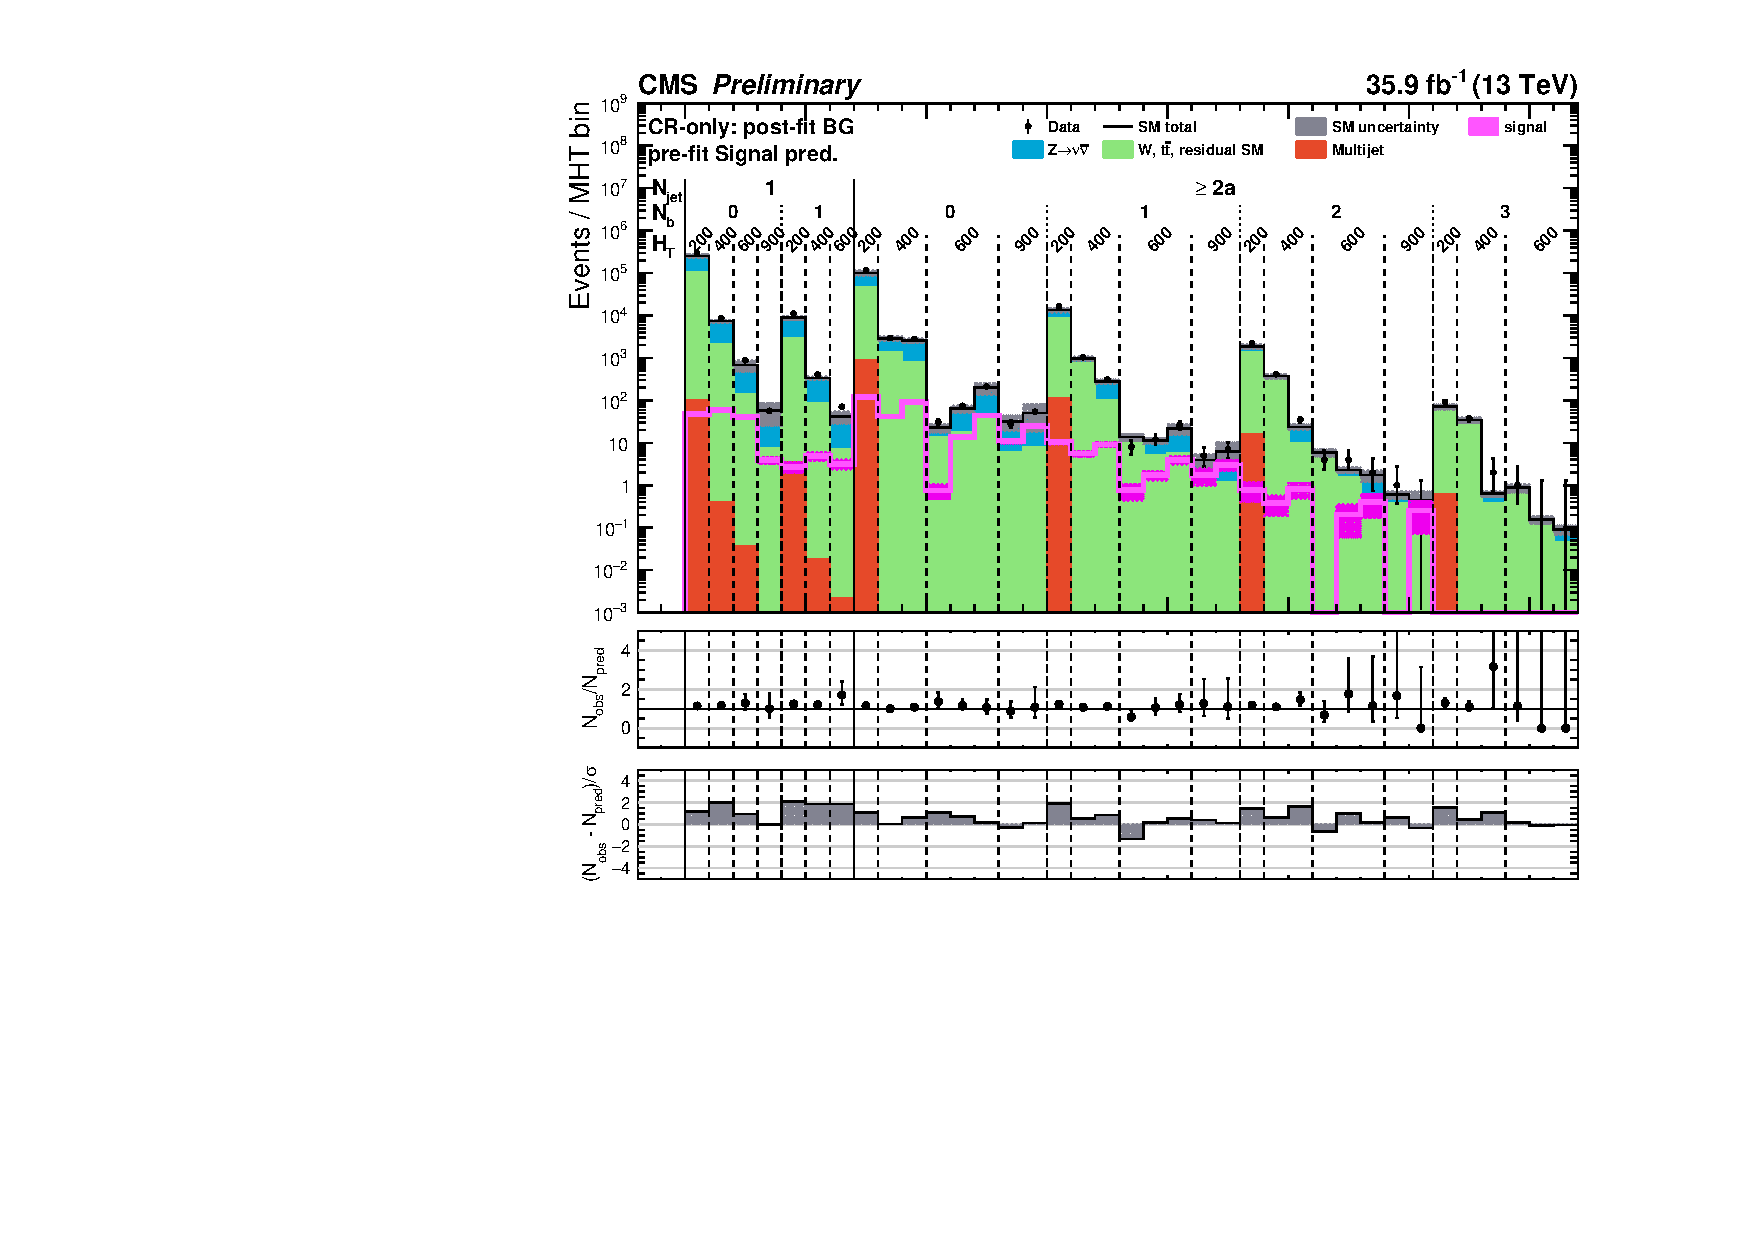
\includegraphics[width=0.49\textwidth]{figures/susyResults/app/T2qq_mSquark-700_mLSP-100/monojet_full-fit-sig}
%        \label{fig:T2qq_1fold_uncompressed_MR_1j}
%    } ~~
%    \subfigure[Di-jet]{
%        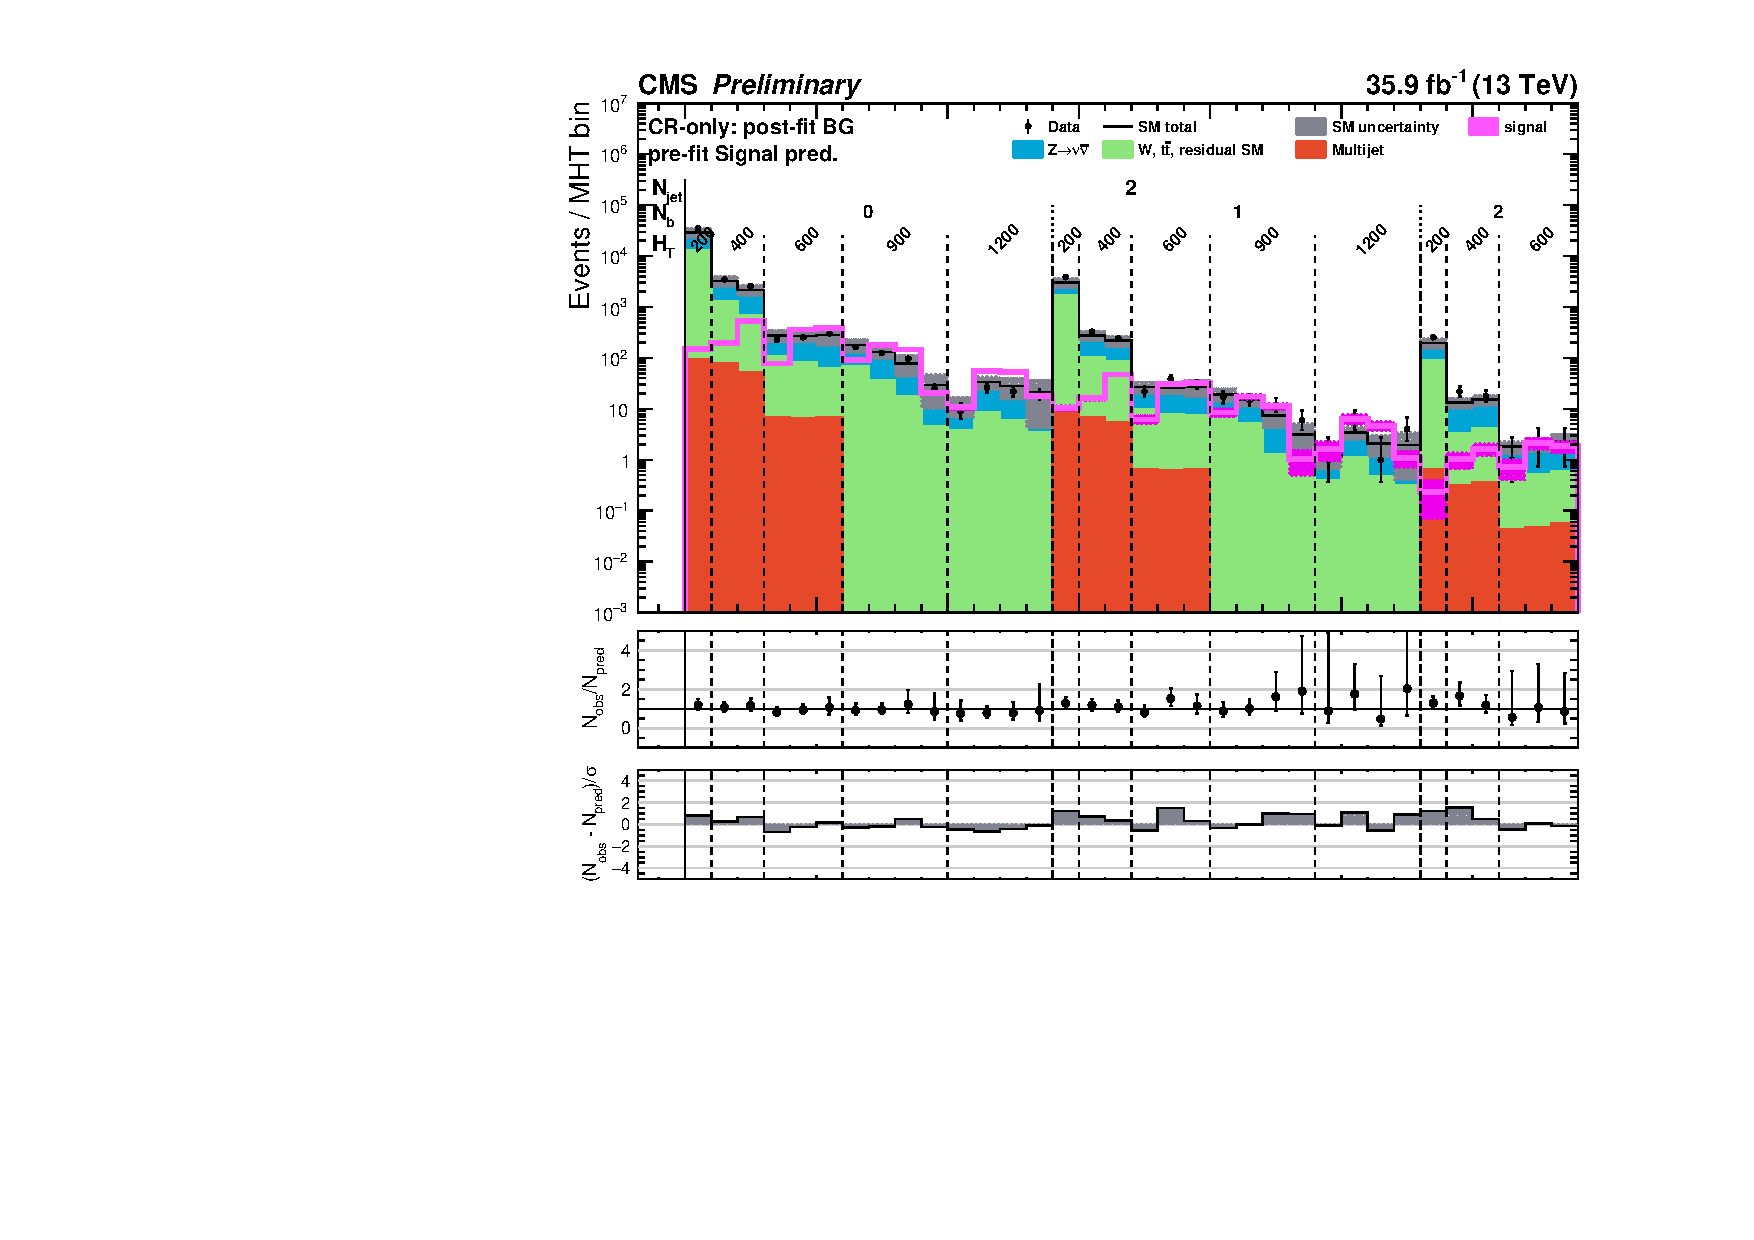
\includegraphics[width=0.49\textwidth]{figures/susyResults/app/T2qq_mSquark-700_mLSP-100/di-jet_full-fit-sig}
%        \label{fig:T2qq_1fold_uncompressed_MR_2j}
%    } \\
%    \subfigure[3 jet]{
%        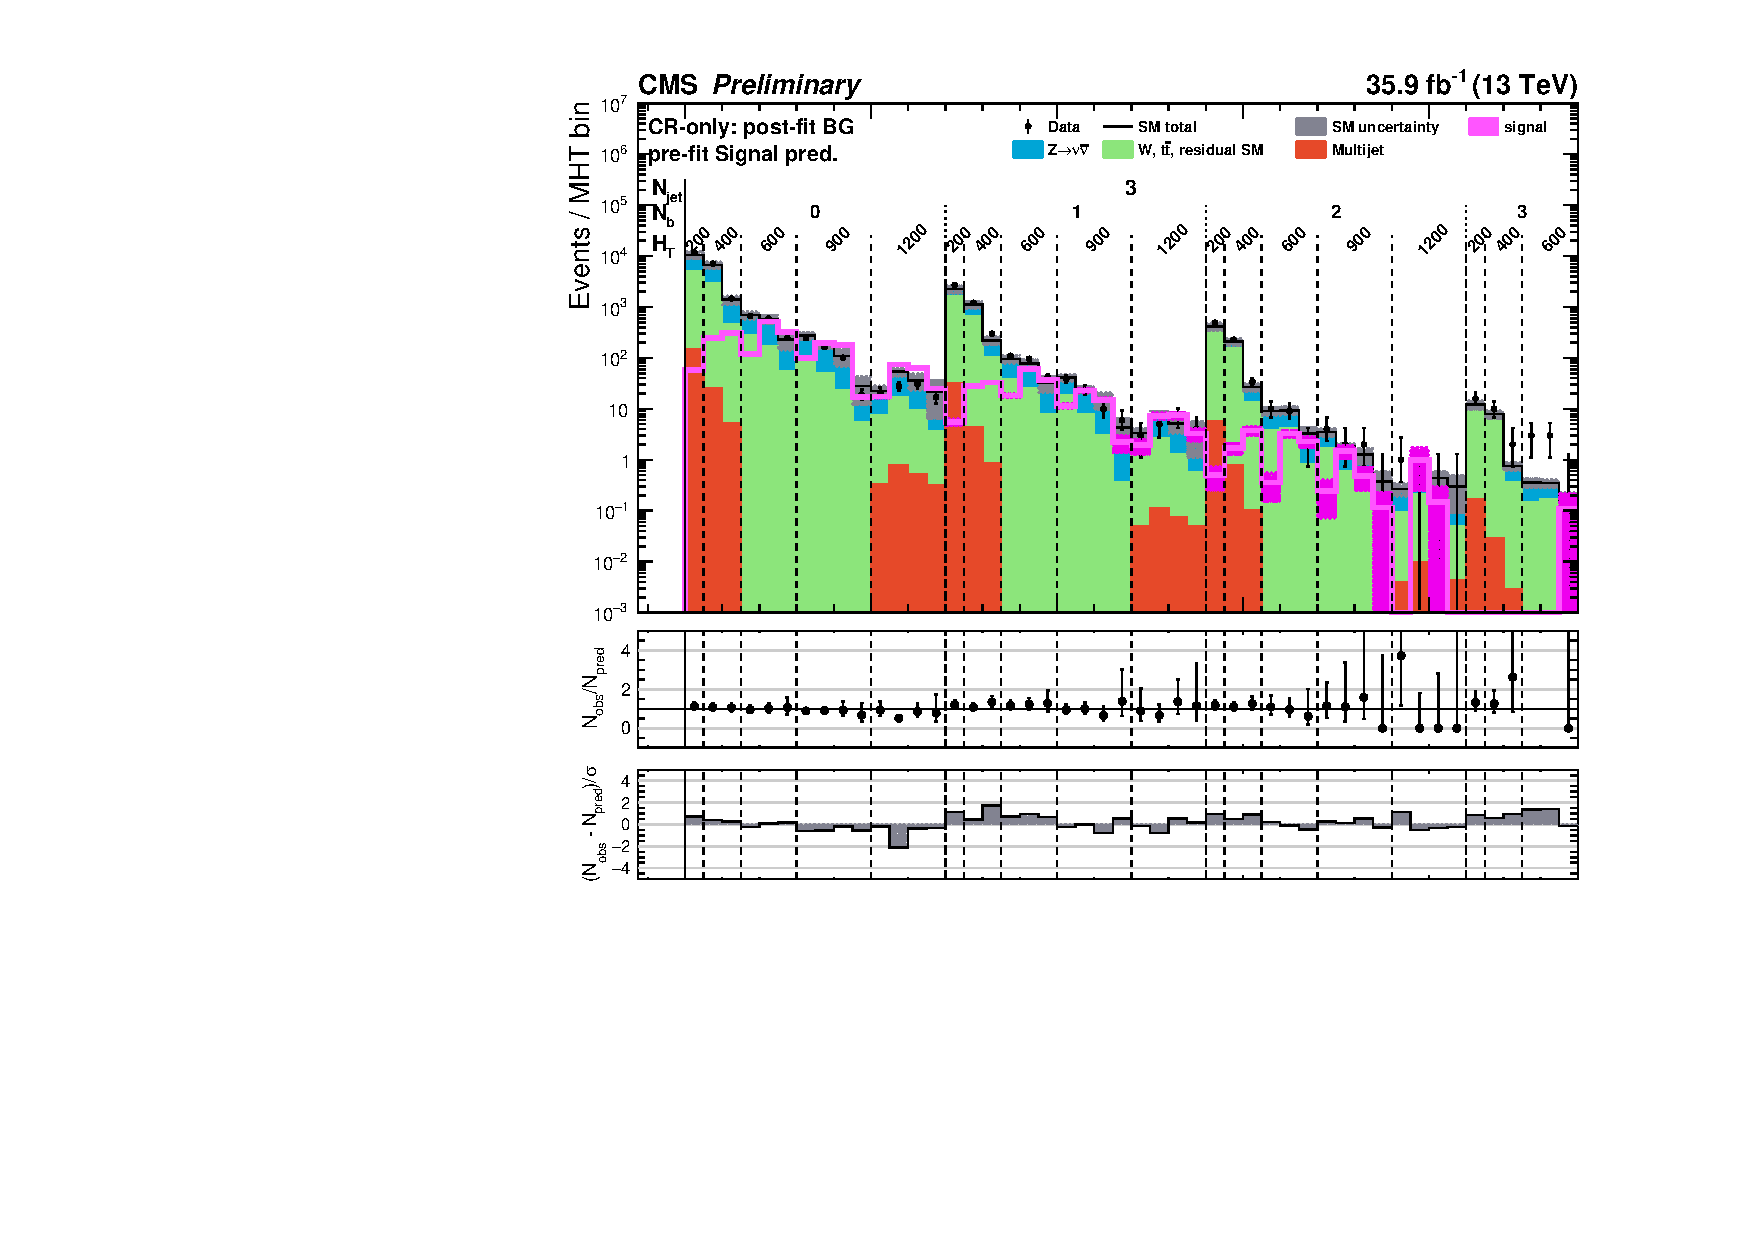
\includegraphics[width=0.49\textwidth]{figures/susyResults/app/T2qq_mSquark-700_mLSP-100/3jet_full-fit-sig}
%        \label{fig:T2qq_1fold_uncompressed_MR_3j}
%    } ~~
%    \subfigure[4 jet]{
%        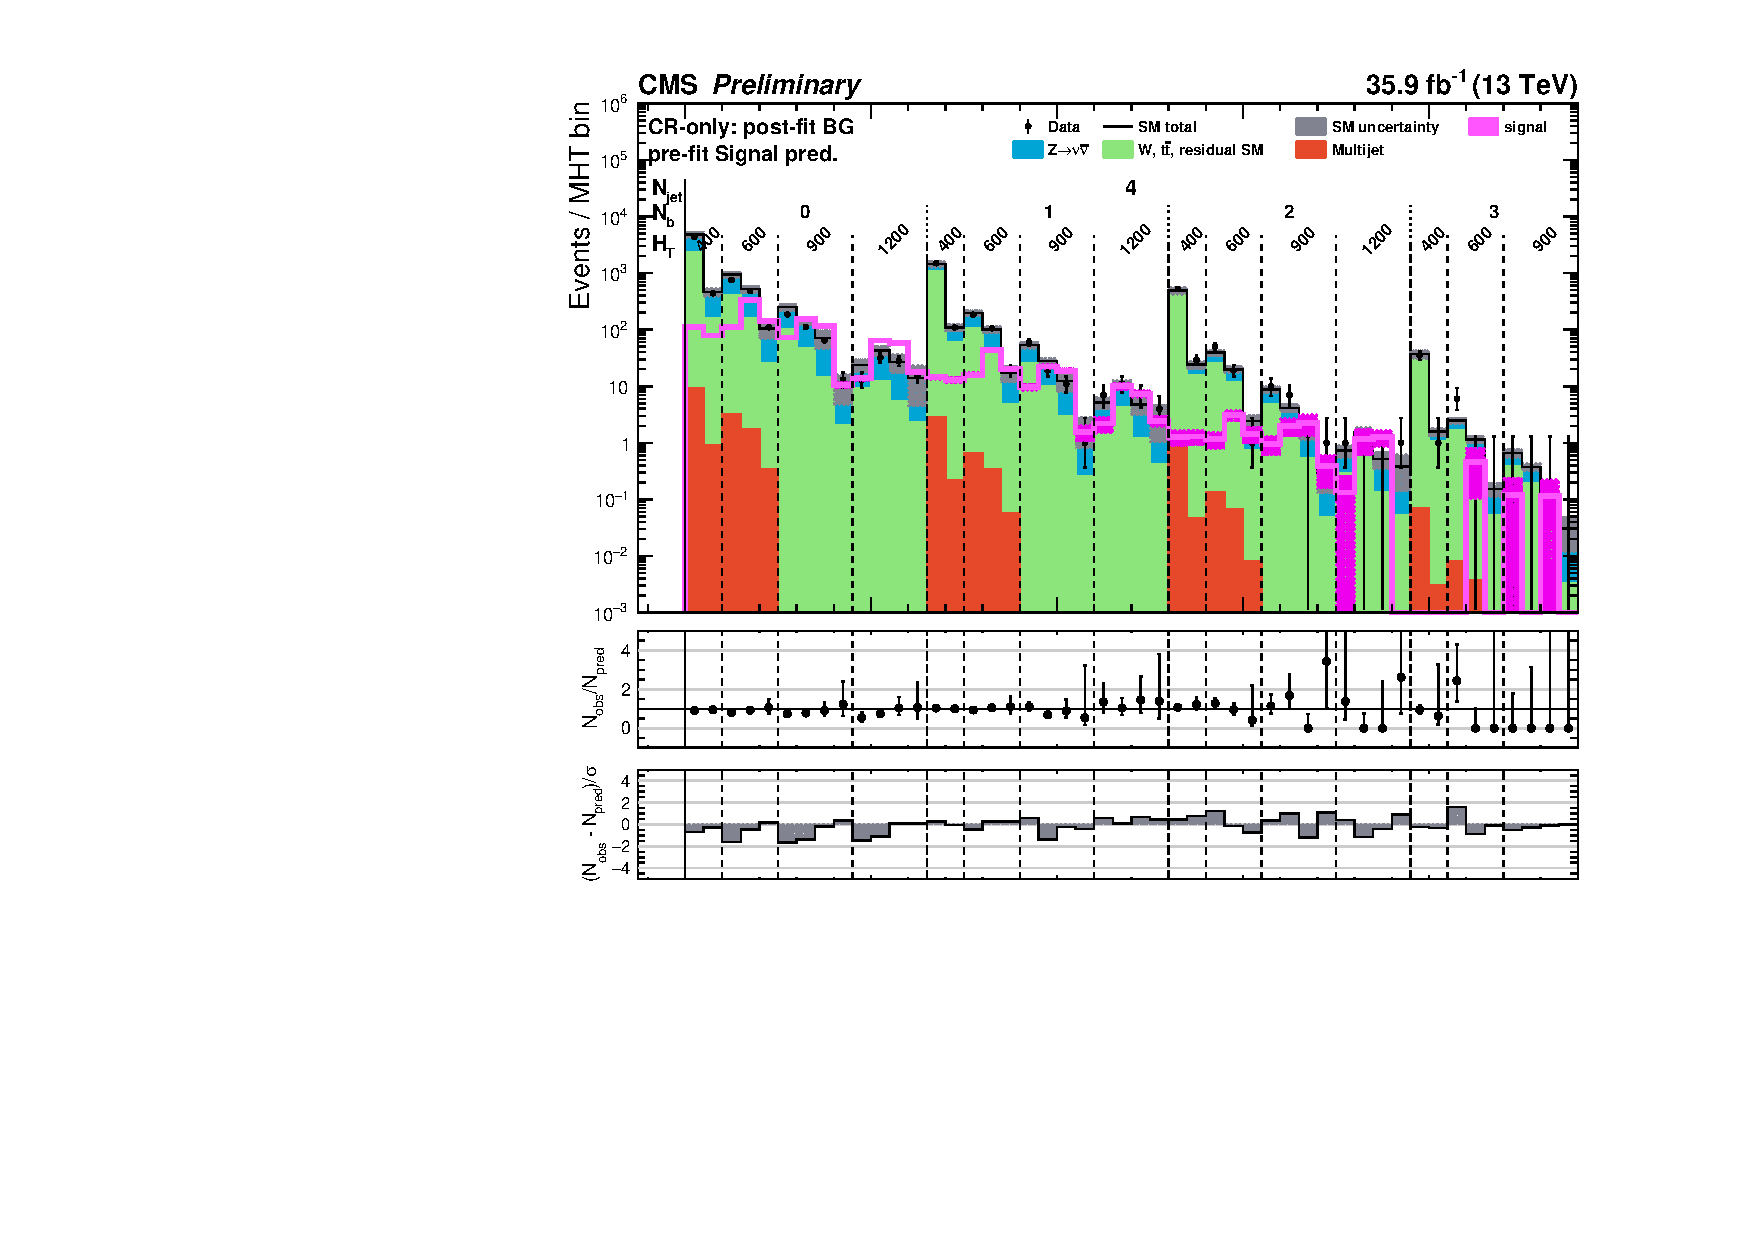
\includegraphics[width=0.49\textwidth]{figures/susyResults/app/T2qq_mSquark-700_mLSP-100/4jet_full-fit-sig}
%        \label{fig:T2qq_1fold_uncompressed_MR_4j}
%    } \\
%    \subfigure[5 jet]{
%        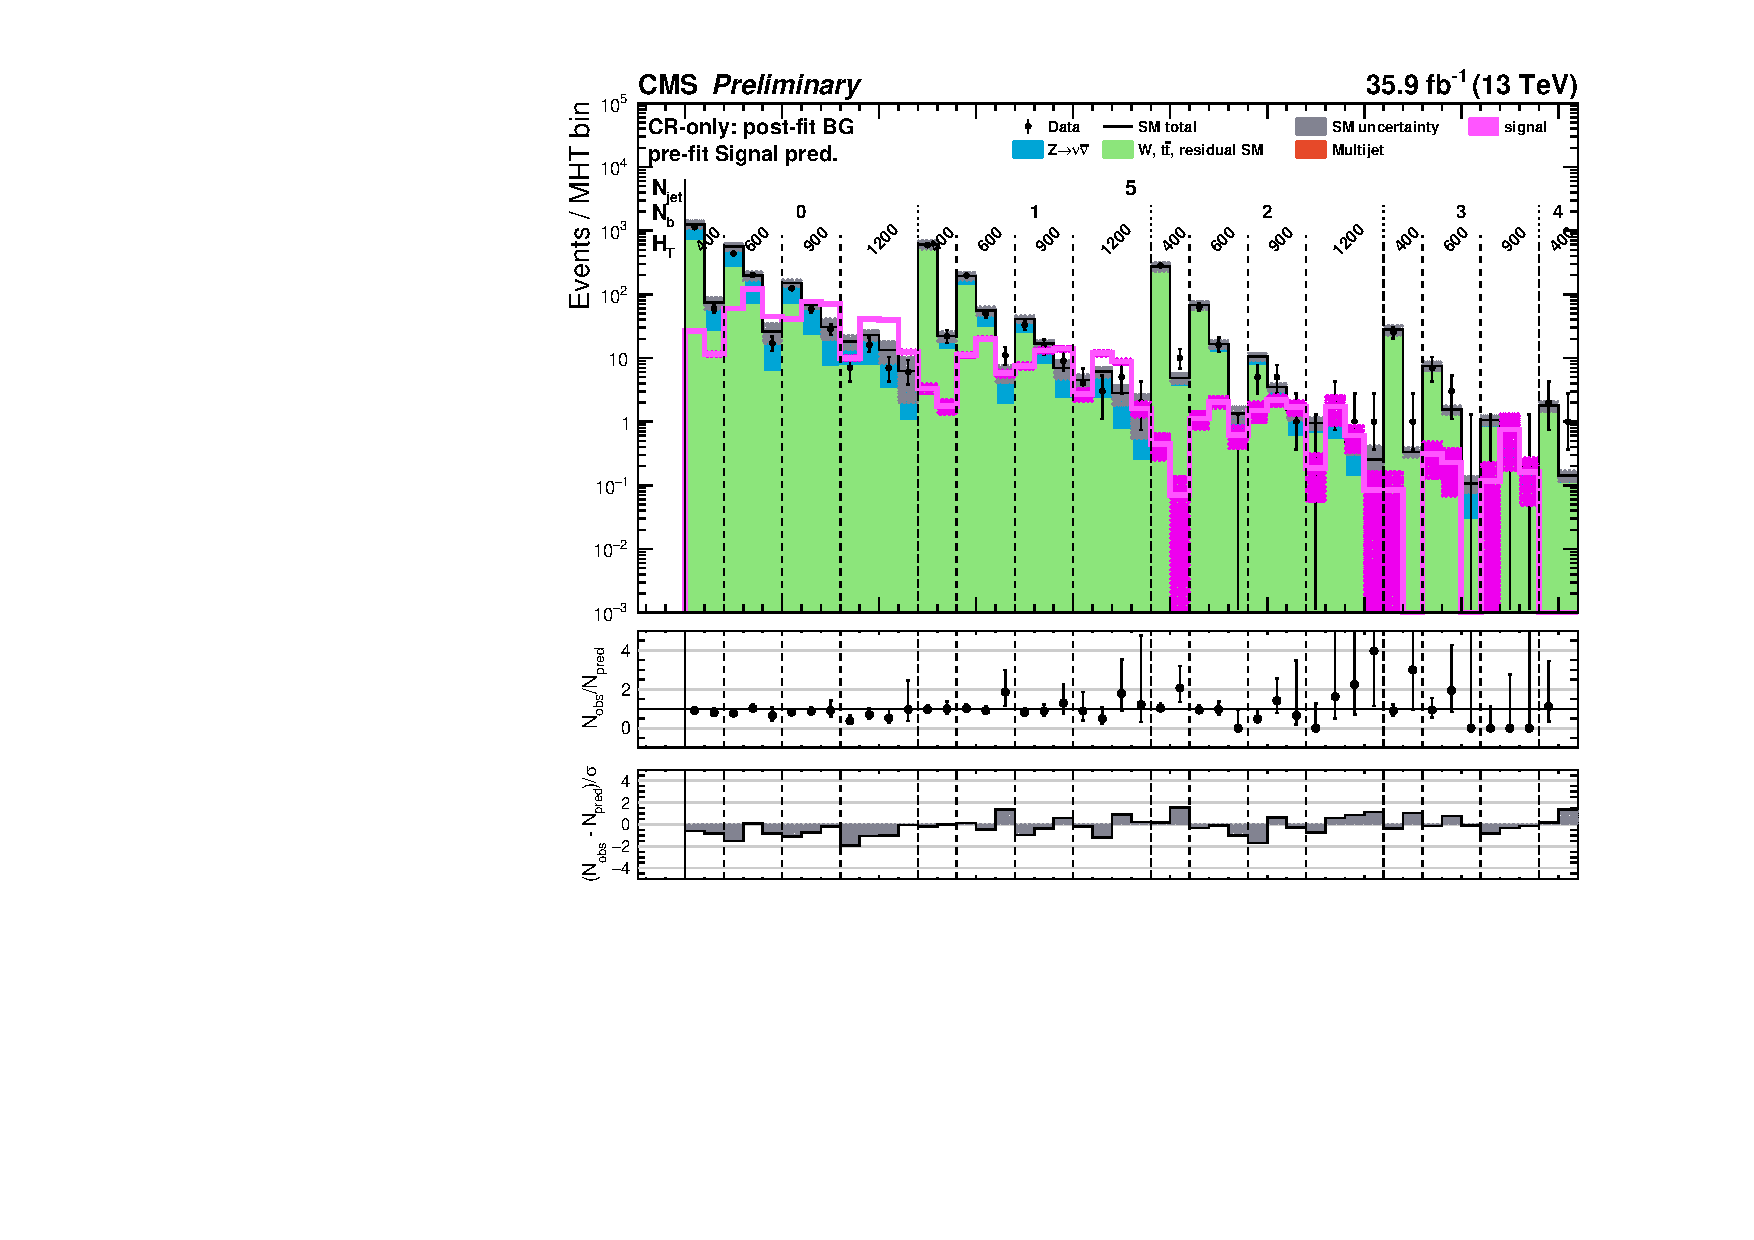
\includegraphics[width=0.49\textwidth]{figures/susyResults/app/T2qq_mSquark-700_mLSP-100/5jet_full-fit-sig}
%        \label{fig:T2qq_1fold_uncompressed_MR_5j}
%    } ~~
%    \subfigure[6+ jet]{
%        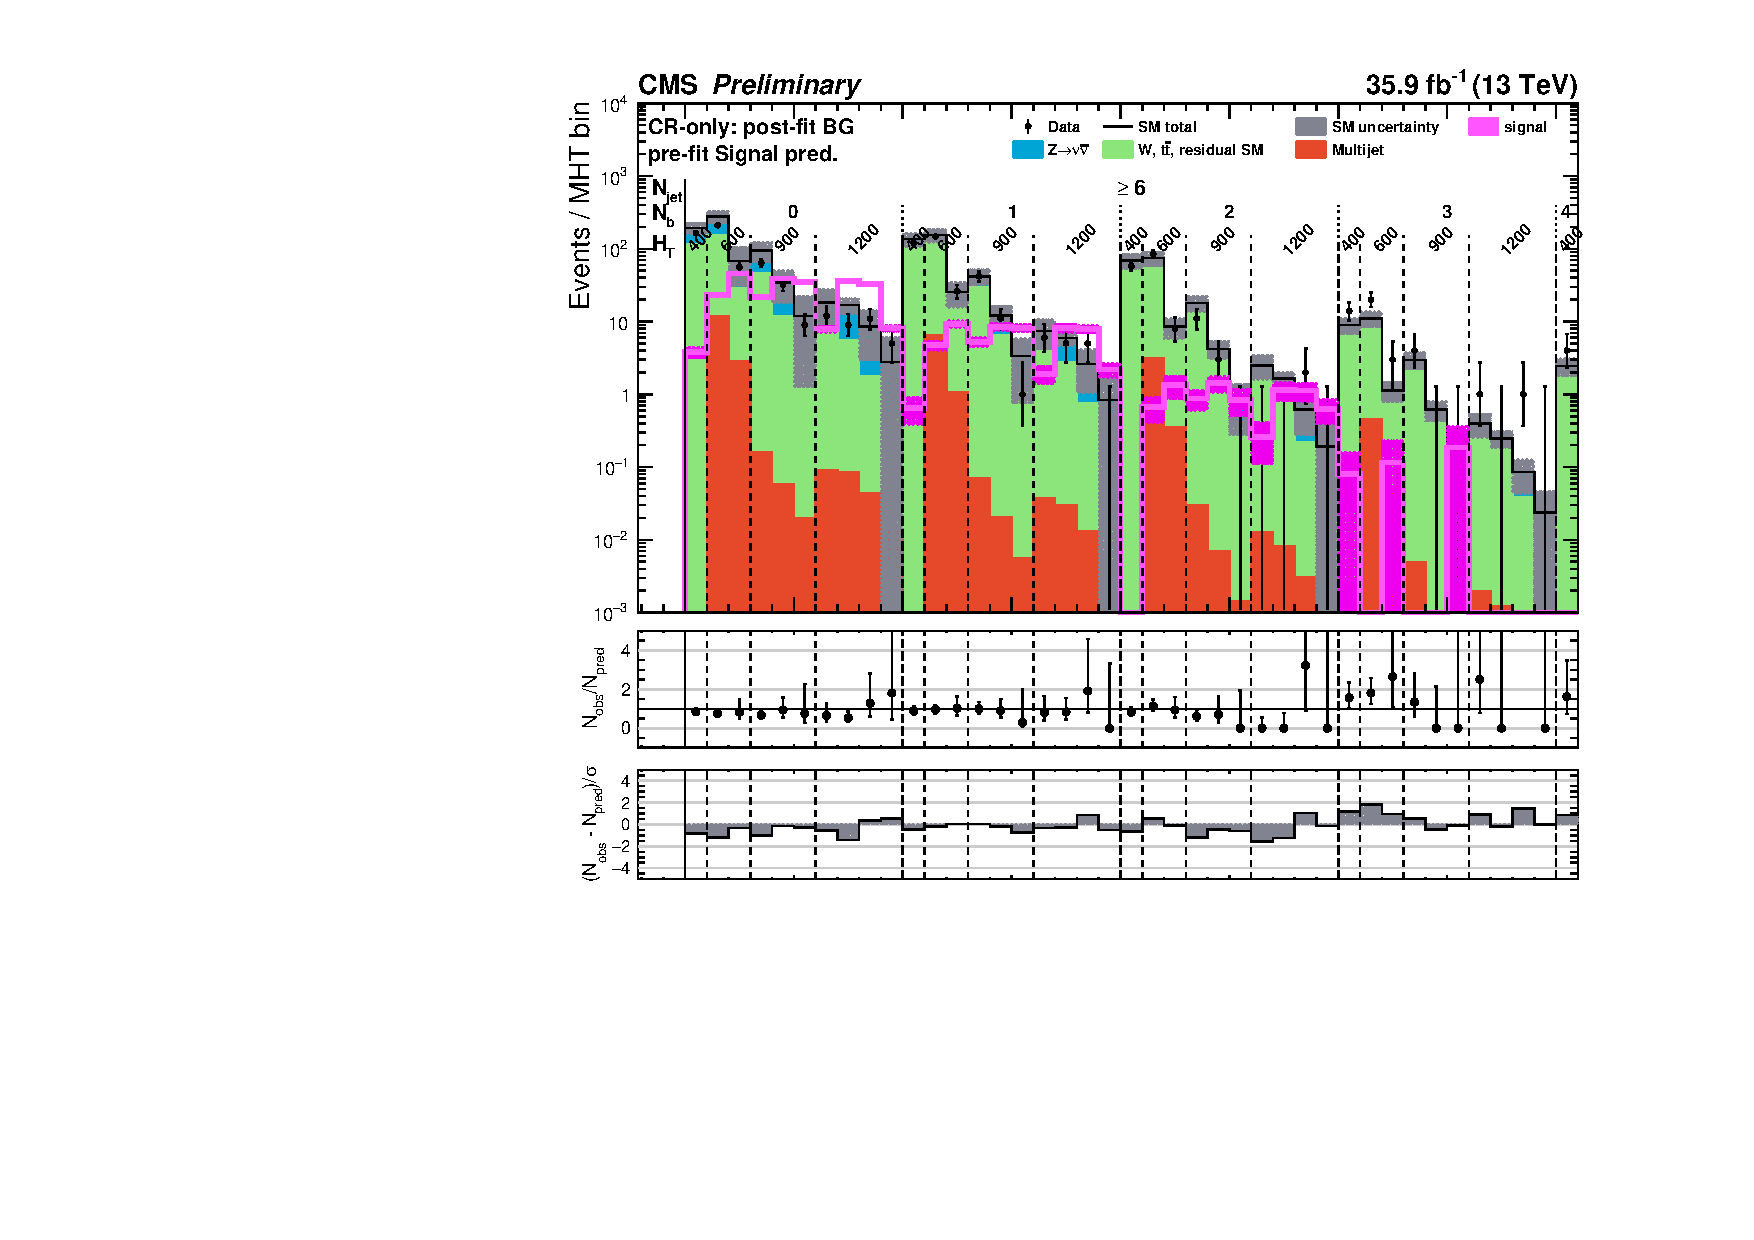
\includegraphics[width=0.49\textwidth]{figures/susyResults/app/T2qq_mSquark-700_mLSP-100/6+_jets_full-fit-sig}
%        \label{fig:T2qq_1fold_uncompressed_MR_6j}
%    } \\
%    \caption{
%        Pre-fit T2qq uncompressed $(700,100)$ benchmark model overlay on CR-only
%        post-fit background prediction for all analysis bins. The uncertainty
%        on the signal model counts represents the statistical uncertainty due
%        to the finite size of the of the simulated sample.
%    }
%    \label{fig:T2qq_1fold_uncompressed_MR}
%\end{figure}
%
%\begin{figure}[!h]
%    \centering
%    \subfigure[Monojet]{
%        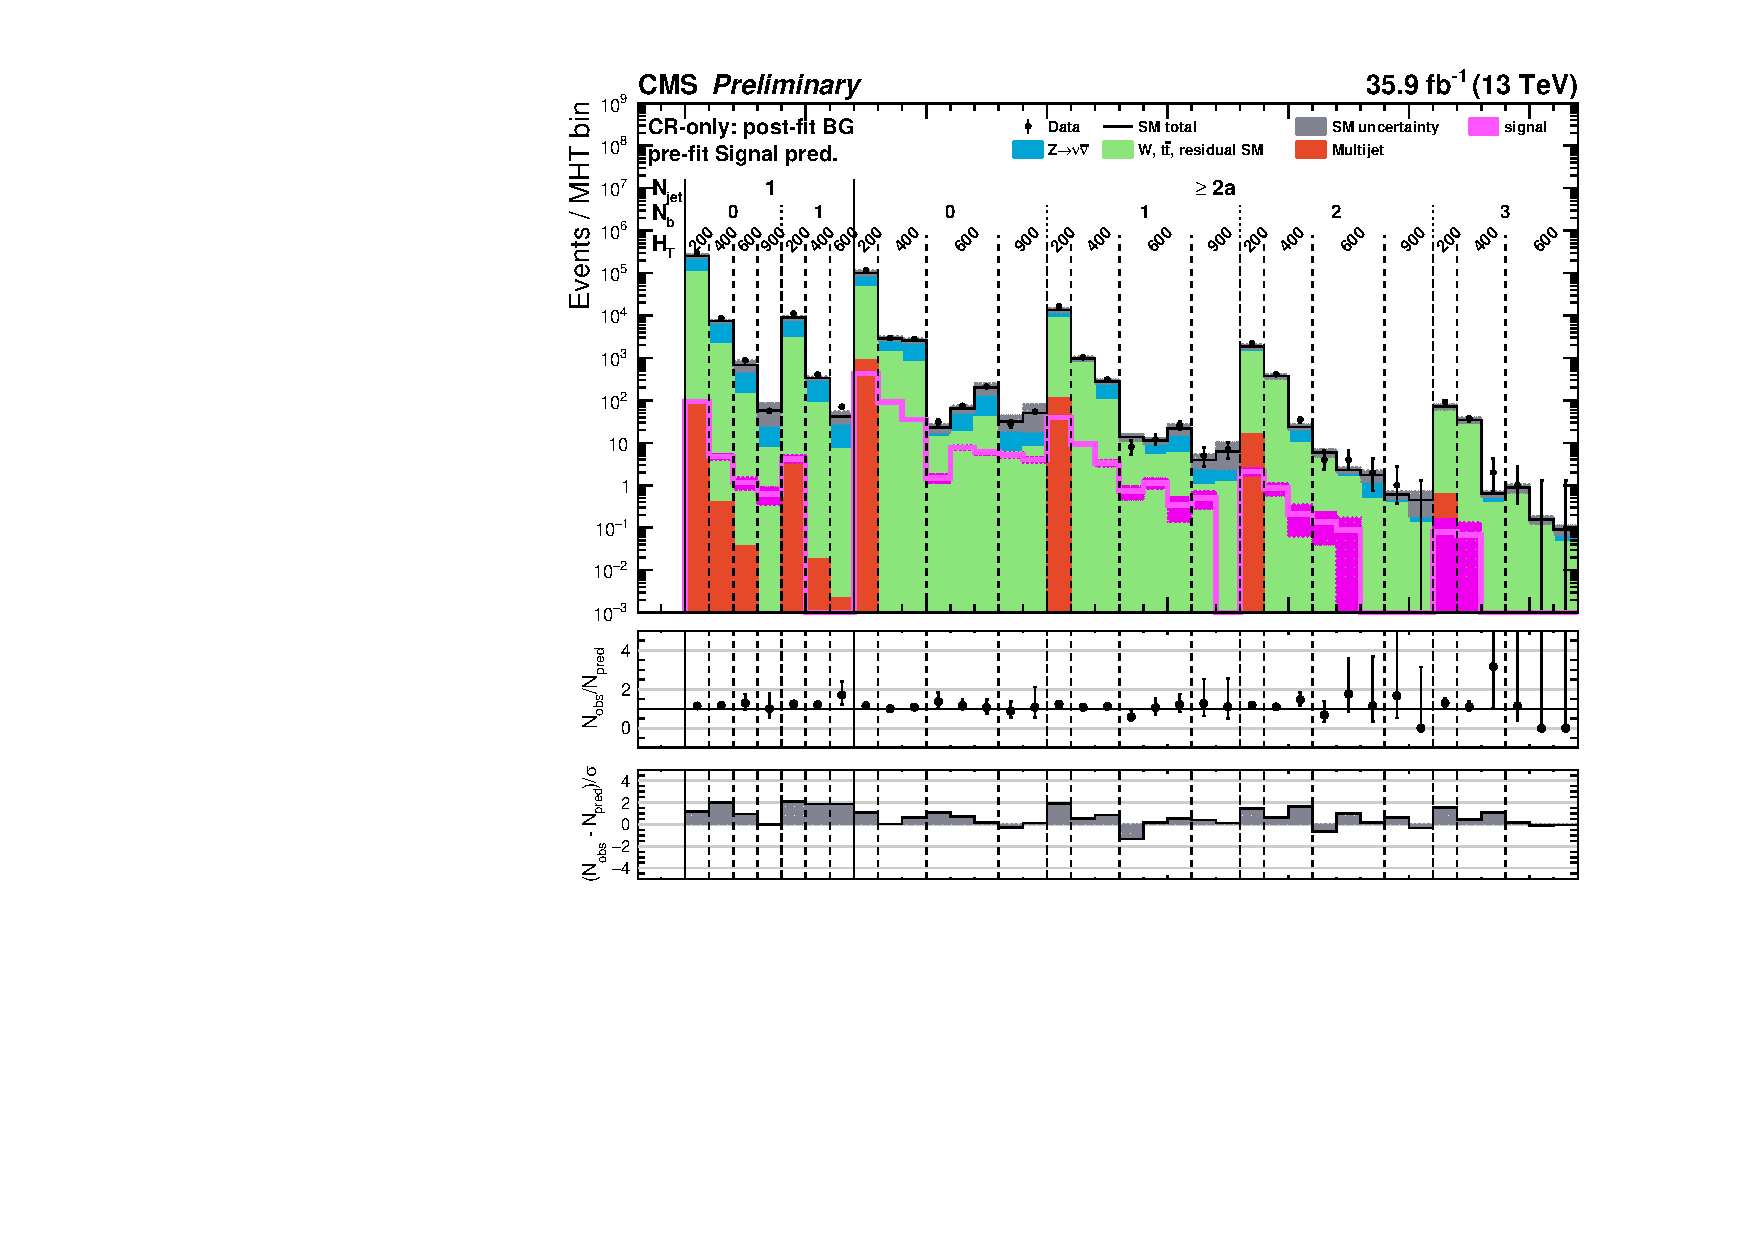
\includegraphics[width=0.49\textwidth]{figures/susyResults/app/T2qq_mSquark-700_mLSP-600/monojet_full-fit-sig}
%        \label{fig:T2qq_8fold_compressed_MR_1j}
%    } ~~
%    \subfigure[Di-jet]{
%        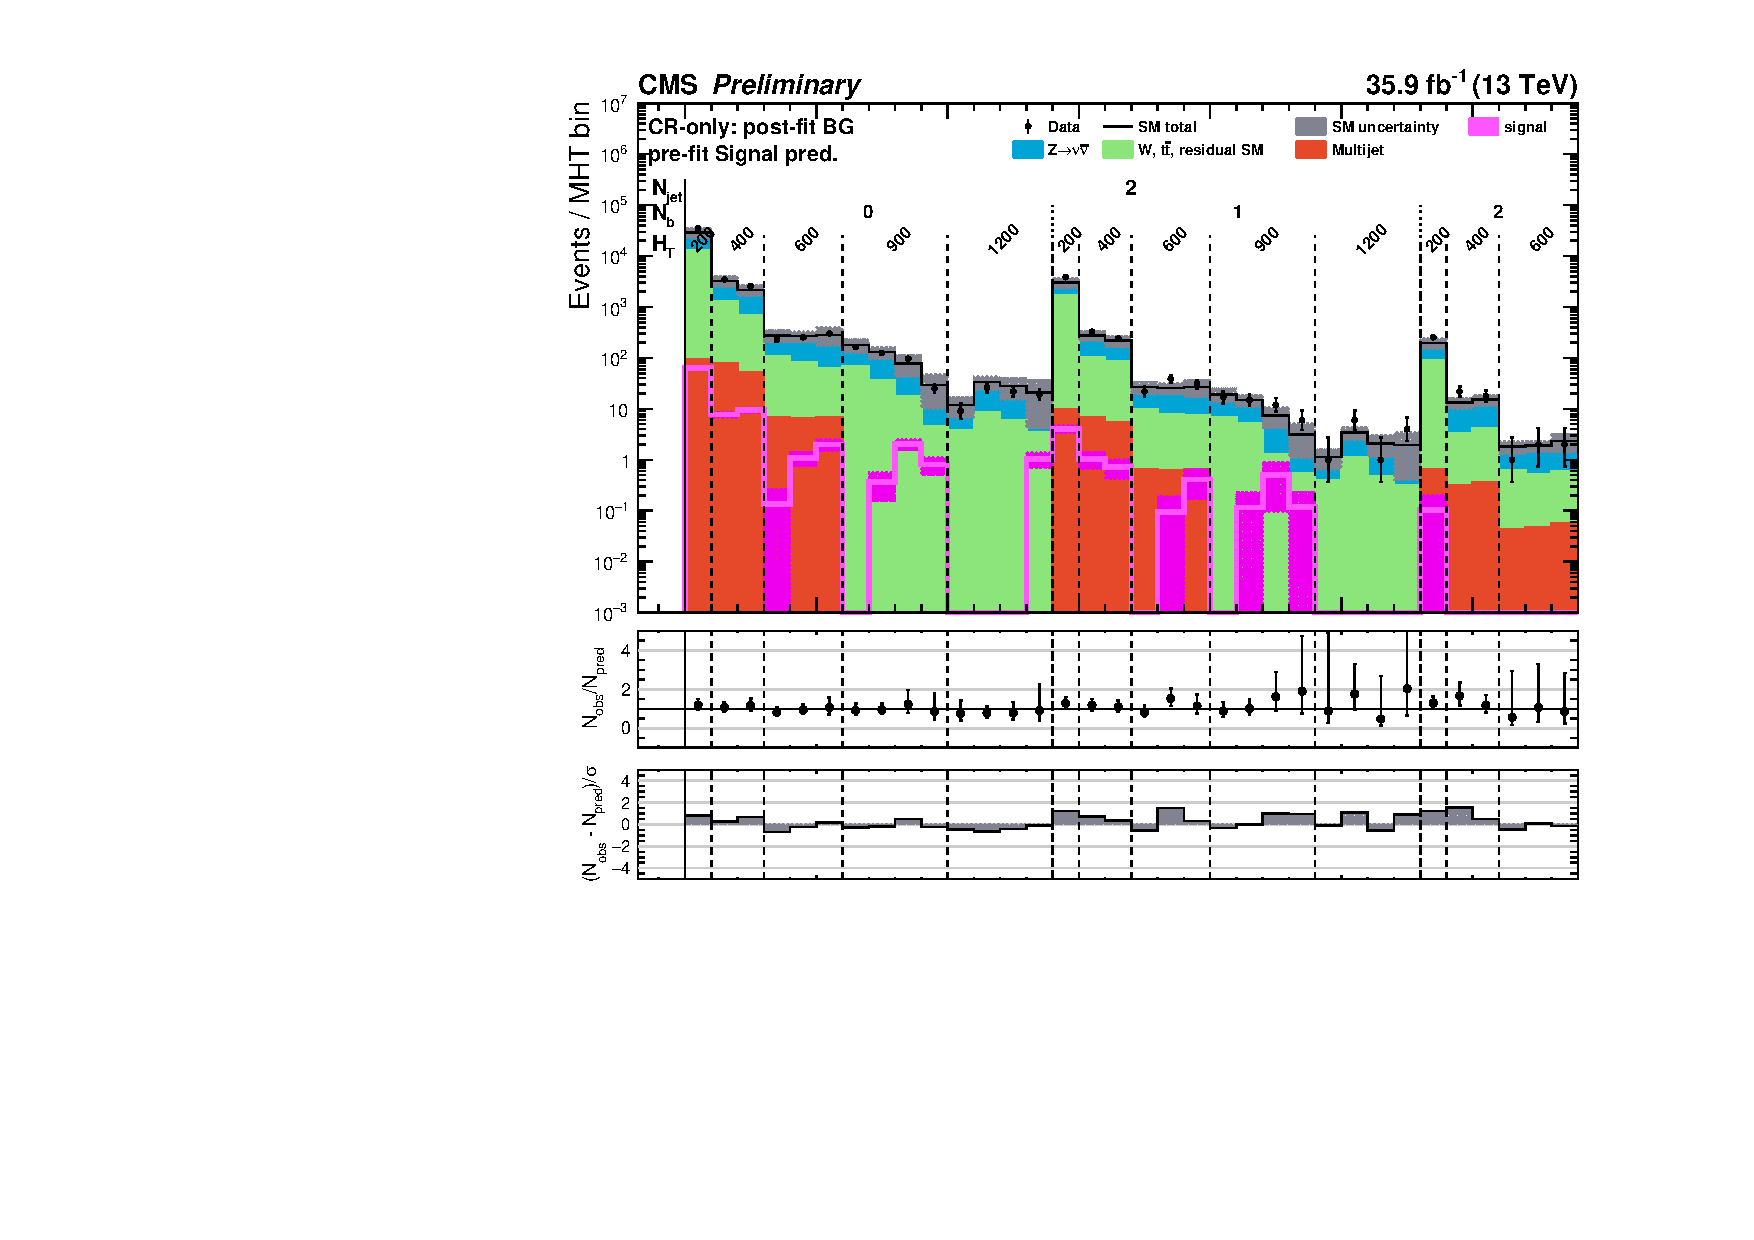
\includegraphics[width=0.49\textwidth]{figures/susyResults/app/T2qq_mSquark-700_mLSP-600/di-jet_full-fit-sig}
%        \label{fig:T2qq_8fold_compressed_MR_2j}
%    } \\
%    \subfigure[3 jet]{
%        \includegraphics[width=0.49\textwidth]{figures/susyResults/app/T2qq_mSquark-700_mLSP-600/3jet_full-fit-sig}
%        \label{fig:T2qq_8fold_compressed_MR_3j}
%    } ~~
%    \subfigure[4 jet]{
%        \includegraphics[width=0.49\textwidth]{figures/susyResults/app/T2qq_mSquark-700_mLSP-600/4jet_full-fit-sig}
%        \label{fig:T2qq_8fold_compressed_MR_4j}
%    } \\
%    \subfigure[5 jet]{
%        \includegraphics[width=0.49\textwidth]{figures/susyResults/app/T2qq_mSquark-700_mLSP-600/5jet_full-fit-sig}
%        \label{fig:T2qq_8fold_compressed_MR_5j}
%    } ~~
%    \subfigure[6+ jet]{
%        \includegraphics[width=0.49\textwidth]{figures/susyResults/app/T2qq_mSquark-700_mLSP-600/6+_jets_full-fit-sig}
%        \label{fig:T2qq_8fold_compressed_MR_6j}
%    } \\
%    \caption{
%        Pre-fit T2qq compressed $(700,600)$ benchmark model overlay on CR-only
%        post-fit background prediction for all analysis bins. The uncertainty
%        on the signal model counts represents the statistical uncertainty due
%        to the finite size of the of the simulated sample.
%    }
%    \label{fig:T2qq_8fold_compressed_MR}
%\end{figure}
%
%\begin{figure}[!h]
%    \centering
%    \subfigure[Monojet]{
%        \includegraphics[width=0.49\textwidth]{figures/susyResults/app/T2qq_mSquark-1250_mLSP-100/monojet_full-fit-sig}
%        \label{fig:T2qq_8fold_uncompressed_MR_1j}
%    } ~~
%    \subfigure[Di-jet]{
%        \includegraphics[width=0.49\textwidth]{figures/susyResults/app/T2qq_mSquark-1250_mLSP-100/di-jet_full-fit-sig}
%        \label{fig:T2qq_8fold_uncompressed_MR_2j}
%    } \\
%    \subfigure[3 jet]{
%        \includegraphics[width=0.49\textwidth]{figures/susyResults/app/T2qq_mSquark-1250_mLSP-100/3jet_full-fit-sig}
%        \label{fig:T2qq_8fold_uncompressed_MR_3j}
%    } ~~
%    \subfigure[4 jet]{
%        \includegraphics[width=0.49\textwidth]{figures/susyResults/app/T2qq_mSquark-1250_mLSP-100/4jet_full-fit-sig}
%        \label{fig:T2qq_8fold_uncompressed_MR_4j}
%    } \\
%    \subfigure[5 jet]{
%        \includegraphics[width=0.49\textwidth]{figures/susyResults/app/T2qq_mSquark-1250_mLSP-100/5jet_full-fit-sig}
%        \label{fig:T2qq_8fold_uncompressed_MR_5j}
%    } ~~
%    \subfigure[6+ jet]{
%        \includegraphics[width=0.49\textwidth]{figures/susyResults/app/T2qq_mSquark-1250_mLSP-100/6+_jets_full-fit-sig}
%        \label{fig:T2qq_8fold_uncompressed_MR_6j}
%    } \\
%    \caption{
%        Pre-fit T2qq uncompressed $(1250,100)$ uncompressed benchmark model
%        overlay on CR-only post-fit background prediction for all analysis bins.
%        The uncertainty on the signal model counts represents the statistical
%        uncertainty due to the finite size of the of the simulated sample.
%    }
%    \label{fig:T2qq_8fold_uncompressed_MR}
%\end{figure}
%
%\begin{figure}[!h]
%    \centering
%    \subfigure[Monojet]{
%        \includegraphics[width=0.49\textwidth]{figures/susyResults/app/T2bb_mSbottom-550_mLSP-450/monojet_full-fit-sig}
%        \label{fig:T2bb_compressed_MR_1j}
%    } ~~
%    \subfigure[Di-jet]{
%        \includegraphics[width=0.49\textwidth]{figures/susyResults/app/T2bb_mSbottom-550_mLSP-450/di-jet_full-fit-sig}
%        \label{fig:T2bb_compressed_MR_2j}
%    } \\
%    \subfigure[3 jet]{
%        \includegraphics[width=0.49\textwidth]{figures/susyResults/app/T2bb_mSbottom-550_mLSP-450/3jet_full-fit-sig}
%        \label{fig:T2bb_compressed_MR_3j}
%    } ~~
%    \subfigure[4 jet]{
%        \includegraphics[width=0.49\textwidth]{figures/susyResults/app/T2bb_mSbottom-550_mLSP-450/4jet_full-fit-sig}
%        \label{fig:T2bb_compressed_MR_4j}
%    } \\
%    \subfigure[5 jet]{
%        \includegraphics[width=0.49\textwidth]{figures/susyResults/app/T2bb_mSbottom-550_mLSP-450/5jet_full-fit-sig}
%        \label{fig:T2bb_compressed_MR_5j}
%    } ~~
%    \subfigure[6+ jet]{
%        \includegraphics[width=0.49\textwidth]{figures/susyResults/app/T2bb_mSbottom-550_mLSP-450/6+_jets_full-fit-sig}
%        \label{fig:T2bb_compressed_MR_6j}
%    } \\
%    \caption{
%        Pre-fit T2bb compressed $(550,450)$ benchmark model overlay on CR-only
%        post-fit background prediction for all analysis bins. The uncertainty
%        on the signal model counts represents the statistical uncertainty due
%        to the finite size of the of the simulated sample.
%    }
%    \label{fig:T2bb_compressed_MR}
%\end{figure}
%
%\begin{figure}[!h]
%    \centering
%    \subfigure[Monojet]{
%        \includegraphics[width=0.49\textwidth]{figures/susyResults/app/T2bb_mSbottom-1000_mLSP-100/monojet_full-fit-sig}
%        \label{fig:T2bb_uncompressed_MR_1j}
%    } ~~
%    \subfigure[Di-jet]{
%        \includegraphics[width=0.49\textwidth]{figures/susyResults/app/T2bb_mSbottom-1000_mLSP-100/di-jet_full-fit-sig}
%        \label{fig:T2bb_uncompressed_MR_2j}
%    } \\
%    \subfigure[3 jet]{
%        \includegraphics[width=0.49\textwidth]{figures/susyResults/app/T2bb_mSbottom-1000_mLSP-100/3jet_full-fit-sig}
%        \label{fig:T2bb_uncompressed_MR_3j}
%    } ~~
%    \subfigure[4 jet]{
%        \includegraphics[width=0.49\textwidth]{figures/susyResults/app/T2bb_mSbottom-1000_mLSP-100/4jet_full-fit-sig}
%        \label{fig:T2bb_uncompressed_MR_4j}
%    } \\
%    \subfigure[5 jet]{
%        \includegraphics[width=0.49\textwidth]{figures/susyResults/app/T2bb_mSbottom-1000_mLSP-100/5jet_full-fit-sig}
%        \label{fig:T2bb_uncompressed_MR_5j}
%    } ~~
%    \subfigure[6+ jet]{
%        \includegraphics[width=0.49\textwidth]{figures/susyResults/app/T2bb_mSbottom-1000_mLSP-100/6+_jets_full-fit-sig}
%        \label{fig:T2bb_uncompressed_MR_6j}
%    } \\
%    \caption{
%        Pre-fit T2bb uncompressed $(1000,100)$ benchmark model overlay on
%        CR-only post-fit background prediction for all analysis bins. The
%        uncertainty on the signal model counts represents the statistical
%        uncertainty due to the finite size of the of the simulated sample.
%    }
%    \label{fig:T2bb_uncompressed_MR}
%\end{figure}
%
%\begin{figure}[!h]
%    \centering
%    \subfigure[Monojet]{
%        \includegraphics[width=0.49\textwidth]{figures/susyResults/app/T2tt_mStop-450_mLSP-200/monojet_full-fit-sig}
%        \label{fig:T2tt_compressed_MR_1j}
%    } ~~
%    \subfigure[Di-jet]{
%        \includegraphics[width=0.49\textwidth]{figures/susyResults/app/T2tt_mStop-450_mLSP-200/di-jet_full-fit-sig}
%        \label{fig:T2tt_compressed_MR_2j}
%    } \\
%    \subfigure[3 jet]{
%        \includegraphics[width=0.49\textwidth]{figures/susyResults/app/T2tt_mStop-450_mLSP-200/3jet_full-fit-sig}
%        \label{fig:T2tt_compressed_MR_3j}
%    } ~~
%    \subfigure[4 jet]{
%        \includegraphics[width=0.49\textwidth]{figures/susyResults/app/T2tt_mStop-450_mLSP-200/4jet_full-fit-sig}
%        \label{fig:T2tt_compressed_MR_4j}
%    } \\
%    \subfigure[5 jet]{
%        \includegraphics[width=0.49\textwidth]{figures/susyResults/app/T2tt_mStop-450_mLSP-200/5jet_full-fit-sig}
%        \label{fig:T2tt_compressed_MR_5j}
%    } ~~
%    \subfigure[6+ jet]{
%        \includegraphics[width=0.49\textwidth]{figures/susyResults/app/T2tt_mStop-450_mLSP-200/6+_jets_full-fit-sig}
%        \label{fig:T2tt_compressed_MR_6j}
%    } \\
%    \caption{
%        Pre-fit T2tt compressed $(450,200)$ benchmark model overlay on CR-only
%        post-fit background prediction for all analysis bins. The uncertainty
%        on the signal model counts represents the statistical uncertainty due
%        to the finite size of the of the simulated sample.
%    }
%    \label{fig:T2tt_compressed_MR}
%\end{figure}
%
%\begin{figure}[!h]
%    \centering
%    \subfigure[Monojet]{
%        \includegraphics[width=0.49\textwidth]{figures/susyResults/app/T2tt_mStop-1000_mLSP-50/monojet_full-fit-sig}
%        \label{fig:T2tt_uncompressed_MR_1j}
%    } ~~
%    \subfigure[Di-jet]{
%        \includegraphics[width=0.49\textwidth]{figures/susyResults/app/T2tt_mStop-1000_mLSP-50/di-jet_full-fit-sig}
%        \label{fig:T2tt_uncompressed_MR_2j}
%    } \\
%    \subfigure[3 jet]{
%        \includegraphics[width=0.49\textwidth]{figures/susyResults/app/T2tt_mStop-1000_mLSP-50/3jet_full-fit-sig}
%        \label{fig:T2tt_uncompressed_MR_3j}
%    } ~~
%    \subfigure[4 jet]{
%        \includegraphics[width=0.49\textwidth]{figures/susyResults/app/T2tt_mStop-1000_mLSP-50/4jet_full-fit-sig}
%        \label{fig:T2tt_uncompressed_MR_4j}
%    } \\
%    \subfigure[5 jet]{
%        \includegraphics[width=0.49\textwidth]{figures/susyResults/app/T2tt_mStop-1000_mLSP-50/5jet_full-fit-sig}
%        \label{fig:T2tt_uncompressed_MR_5j}
%    } ~~
%    \subfigure[6+ jet]{
%        \includegraphics[width=0.49\textwidth]{figures/susyResults/app/T2tt_mStop-1000_mLSP-50/6+_jets_full-fit-sig}
%        \label{fig:T2tt_uncompressed_MR_6j}
%    } \\
%    \caption{
%        Pre-fit T2tt uncompressed $(1000,50)$ benchmark model overlay on
%        CR-only post-fit background prediction for all analysis bins. The
%        uncertainty on the signal model counts represents the statistical
%        uncertainty due to the finite size of the of the simulated sample.
%    }
%    \label{fig:T2tt_uncompressed_MR}
%\end{figure}
%
%\begin{figure}[!h]
%    \centering
%    \subfigure[Monojet]{
%        \includegraphics[width=0.49\textwidth]{figures/susyResults/app/T2tt_mStop-250_mLSP-150/monojet_full-fit-sig}
%        \label{fig:T2tt_Wcorridor_MR_1j}
%    } ~~
%    \subfigure[Di-jet]{
%        \includegraphics[width=0.49\textwidth]{figures/susyResults/app/T2tt_mStop-250_mLSP-150/di-jet_full-fit-sig}
%        \label{fig:T2tt_Wcorridor_MR_2j}
%    } \\
%    \subfigure[3 jet]{
%        \includegraphics[width=0.49\textwidth]{figures/susyResults/app/T2tt_mStop-250_mLSP-150/3jet_full-fit-sig}
%        \label{fig:T2tt_Wcorridor_MR_3j}
%    } ~~
%    \subfigure[4 jet]{
%        \includegraphics[width=0.49\textwidth]{figures/susyResults/app/T2tt_mStop-250_mLSP-150/4jet_full-fit-sig}
%        \label{fig:T2tt_Wcorridor_MR_4j}
%    } \\
%    \subfigure[5 jet]{
%        \includegraphics[width=0.49\textwidth]{figures/susyResults/app/T2tt_mStop-250_mLSP-150/5jet_full-fit-sig}
%        \label{fig:T2tt_Wcorridor_MR_5j}
%    } ~~
%    \subfigure[6+ jet]{
%        \includegraphics[width=0.49\textwidth]{figures/susyResults/app/T2tt_mStop-250_mLSP-150/6+_jets_full-fit-sig}
%        \label{fig:T2tt_Wcorridor_MR_6j}
%    } \\
%    \caption{
%        Pre-fit T2tt $W$ corridor $(250,150)$ benchmark model overlay on
%        CR-only post-fit background prediction for all analysis bins. The
%        uncertainty on the signal model counts represents the statistical
%        uncertainty due to the finite size of the of the simulated sample.
%    }
%    \label{fig:T2tt_Wcorridor_MR}
%\end{figure}
%
%\begin{figure}[!h]
%    \centering
%    \subfigure[Monojet]{
%        \includegraphics[width=0.49\textwidth]{figures/susyResults/app/T2cc_mStop-500_mLSP-480/monojet_full-fit-sig}
%        \label{fig:T2cc_compressed_MR_1j}
%    } ~~
%    \subfigure[Di-jet]{
%        \includegraphics[width=0.49\textwidth]{figures/susyResults/app/T2cc_mStop-500_mLSP-480/di-jet_full-fit-sig}
%        \label{fig:T2cc_compressed_MR_2j}
%    } \\
%    \subfigure[3 jet]{
%        \includegraphics[width=0.49\textwidth]{figures/susyResults/app/T2cc_mStop-500_mLSP-480/3jet_full-fit-sig}
%        \label{fig:T2cc_compressed_MR_3j}
%    } ~~
%    \subfigure[4 jet]{
%        \includegraphics[width=0.49\textwidth]{figures/susyResults/app/T2cc_mStop-500_mLSP-480/4jet_full-fit-sig}
%        \label{fig:T2cc_compressed_MR_4j}
%    } \\
%    \subfigure[5 jet]{
%        \includegraphics[width=0.49\textwidth]{figures/susyResults/app/T2cc_mStop-500_mLSP-480/5jet_full-fit-sig}
%        \label{fig:T2cc_compressed_MR_5j}
%    } ~~
%    \subfigure[6+ jet]{
%        \includegraphics[width=0.49\textwidth]{figures/susyResults/app/T2cc_mStop-500_mLSP-480/6+_jets_full-fit-sig}
%        \label{fig:T2cc_compressed_MR_6j}
%    } \\
%    \caption{
%        Pre-fit T2cc $(500,480)$ benchmark model overlay on CR-only post-fit
%        background prediction for all analysis bins. The uncertainty on the
%        signal model counts represents the statistical uncertainty due to the
%        finite size of the of the simulated sample.
%    }
%    \label{fig:T2cc_compressed_MR}
%\end{figure}
%
%
%\clearpage
%\subsubsection{Simplified binning}

\begin{figure}[!h]
    \centering
    \subfigure[Compressed $(1000,850)$]{
        \includegraphics[width=0.7\textwidth]{figures/susyResults/app/T1qqqq_mGluino-1000_mLSP-850/all_full-fit-sig}
        \label{fig:T1qqqq_compressed_MR_simp}
    } \\
    \subfigure[Uncompressed $(1700,100)$]{
        \includegraphics[width=0.7\textwidth]{figures/susyResults/app/T1qqqq_mGluino-1700_mLSP-100/all_full-fit-sig}
        \label{fig:T1qqqq_uncompressed_MR_simp}
    }
    \caption{
        Pre-fit T1qqqq benchmark model overlay on CR-only post-fit
        background prediction for the simplified bins. The uncertainty on
        the signal model counts represents the statistical uncertainty due
        to the finite size of the of the simulated sample.
    }
    \label{fig:T1qqqq_MR_simp}
\end{figure}

\begin{figure}[!h]
    \centering
    \subfigure[Compressed]{
        \includegraphics[width=0.7\textwidth]{figures/susyResults/app/T1bbbb_mGluino-1300_mLSP-1100/all_full-fit-sig}
        \label{fig:T1bbbb_compressed_MR_simp}
    } \\
    \subfigure[Uncompressed]{
        \includegraphics[width=0.7\textwidth]{figures/susyResults/app/T1bbbb_mGluino-1900_mLSP-100/all_full-fit-sig}
        \label{fig:T1bbbb_uncompressed_MR_simp}
    }
    \caption{
        Pre-fit T1bbbb benchmark model overlay on CR-only post-fit
        background prediction for the simplified bins. The uncertainty on
        the signal model counts represents the statistical uncertainty due
        to the finite size of the of the simulated sample.
    }
    \label{fig:T1bbbb_MR_simp}
\end{figure}

\begin{figure}[!h]
    \centering
    \subfigure[Compressed]{
        \includegraphics[width=0.7\textwidth]{figures/susyResults/app/T1tttt_mGluino-950_mLSP-600/all_full-fit-sig}
        \label{fig:T1tttt_compressed_MR_simp}
    } \\
    \subfigure[Uncompressed]{
        \includegraphics[width=0.7\textwidth]{figures/susyResults/app/T1tttt_mGluino-1700_mLSP-100/all_full-fit-sig}
        \label{fig:T1tttt_uncompressed_MR_simp}
    }
    \caption{
        Pre-fit T1tttt benchmark model overlay on CR-only post-fit
        background prediction for the simplified bins. The uncertainty on
        the signal model counts represents the statistical uncertainty due
        to the finite size of the of the simulated sample.
    }
    \label{fig:T1tttt_MR_simp}
\end{figure}

\begin{figure}[!h]
    \centering
    \subfigure[Compressed]{
        \includegraphics[width=0.7\textwidth]{figures/susyResults/app/T2qq_mSquark-400_mLSP-300/all_full-fit-sig}
        \label{fig:T2qq_1fold_compressed_MR_simp}
    } \\
    \subfigure[Uncompressed]{
        \includegraphics[width=0.7\textwidth]{figures/susyResults/app/T2qq_mSquark-700_mLSP-100/all_full-fit-sig}
        \label{fig:T2qq_1fold_uncompressed_MR_simp}
    }
    \caption{
        Pre-fit T2qq benchmark model overlay on CR-only post-fit
        background prediction for the simplified bins. The uncertainty on
        the signal model counts represents the statistical uncertainty due
        to the finite size of the of the simulated sample.
    }
    \label{fig:T2qq_1fold_MR_simp}
\end{figure}

\begin{figure}[!h]
    \centering
    \subfigure[Compressed]{
        \includegraphics[width=0.7\textwidth]{figures/susyResults/app/T2qq_mSquark-700_mLSP-600/all_full-fit-sig}
        \label{fig:T2qq_8fold_compressed_MR_simp}
    } \\
    \subfigure[Uncompressed]{
        \includegraphics[width=0.7\textwidth]{figures/susyResults/app/T2qq_mSquark-1250_mLSP-100/all_full-fit-sig}
        \label{fig:T2qq_8fold_uncompressed_MR_simp}
    }
    \caption{
        Pre-fit T2qq benchmark model overlay on CR-only post-fit
        background prediction for the simplified bins. The uncertainty on
        the signal model counts represents the statistical uncertainty due
        to the finite size of the of the simulated sample.
    }
    \label{fig:T2qq_8fold_MR_simp}
\end{figure}

\begin{figure}[!h]
    \centering
    \subfigure[Compressed]{
        \includegraphics[width=0.7\textwidth]{figures/susyResults/app/T2bb_mSbottom-550_mLSP-450/all_full-fit-sig}
        \label{fig:T2bb_compressed_MR_simp}
    } \\
    \subfigure[Uncompressed]{
        \includegraphics[width=0.7\textwidth]{figures/susyResults/app/T2bb_mSbottom-1000_mLSP-100/all_full-fit-sig}
        \label{fig:T2bb_uncompressed_MR_simp}
    }
    \caption{
        Pre-fit T2bb benchmark model overlay on CR-only post-fit
        background prediction for the simplified bins. The uncertainty on
        the signal model counts represents the statistical uncertainty due
        to the finite size of the of the simulated sample.
    }
    \label{fig:T2bb_MR_simp}
\end{figure}

\begin{figure}[!h]
    \centering
    \subfigure[Compressed]{
        \includegraphics[width=0.49\textwidth]{figures/susyResults/app/T2tt_mStop-450_mLSP-200/all_full-fit-sig}
        \label{fig:T2tt_compressed_MR_simp}
    } ~~
    \subfigure[Uncompressed]{
        \includegraphics[width=0.49\textwidth]{figures/susyResults/app/T2tt_mStop-1000_mLSP-50/all_full-fit-sig}
        \label{fig:T2tt_uncompressed_MR_simp}
    } \\
    \subfigure[$W$ corridor]{
        \includegraphics[width=0.49\textwidth]{figures/susyResults/app/T2tt_mStop-250_mLSP-150/all_full-fit-sig}
        \label{fig:T2tt_Wcorridor_MR_simp}
    }
    \caption{
        Pre-fit T2tt benchmark model overlay on CR-only post-fit
        background prediction for the simplified bins. The uncertainty on
        the signal model counts represents the statistical uncertainty due
        to the finite size of the of the simulated sample.
    }
    \label{fig:T2tt_MR_simp}
\end{figure}

\begin{figure}[!h]
    \centering
    \subfigure[Compressed]{
        \includegraphics[width=0.7\textwidth]{figures/susyResults/app/T2cc_mStop-500_mLSP-480/all_full-fit-sig}
        \label{fig:T2cc_compressed_MR_simp}
    }
    \caption{
        Pre-fit T2cc benchmark model overlay on CR-only post-fit
        background prediction for the simplified bins. The uncertainty on
        the signal model counts represents the statistical uncertainty due
        to the finite size of the of the simulated sample.
    }
    \label{fig:T2cc_MR_simp}
\end{figure}
